\documentclass[12pt]{article}

% --- ESSENTIAL PACKAGES ---
\usepackage[a4paper, margin=1in]{geometry}
\usepackage{graphicx}
\usepackage{booktabs}
\usepackage{longtable}
\usepackage{pdflscape}
\usepackage{subfig}
\usepackage{multirow}
\usepackage{array}
\usepackage[nottoc]{tocbibind}
\usepackage{hyperref}

% --- HYPERLINK FORMATTING ---
\hypersetup{
    colorlinks=true,
    linkcolor=black,
    filecolor=black,      
    urlcolor=black,
    citecolor=black,
}

% --- GRAPHICS PATH ---
\graphicspath{{figures/final/}} 

% --- TITLE BLOCK ---
\title{Supplementary Information for: \\ \textbf{DIANA: Deep Learning Identification and Assessment of Ancient DNA}}
\author{Camila Duitama González et al.}
\date{}

% =================================================================
%                        START OF DOCUMENT
% =================================================================
\begin{document}

\maketitle

\tableofcontents
\clearpage

\listoffigures
\clearpage

\listoftables
\clearpage

% --- RENAME & RESET COUNTERS ---
\renewcommand{\figurename}{Supplementary Figure}
\renewcommand{\tablename}{Supplementary Table}
\setcounter{figure}{0}
\setcounter{table}{0}

%%%%%%%%%%%%%%%%%%%%%%%%%%%%%%%%%%%%%%%%%%%%%%%%%%%%%%%%%%%%%%%%%%%%%
%                       SUPPLEMENTARY TABLES                        %
%%%%%%%%%%%%%%%%%%%%%%%%%%%%%%%%%%%%%%%%%%%%%%%%%%%%%%%%%%%%%%%%%%%%%
\section{Supplementary Tables}

% Sup Table 01: Class Distribution (longtable - no table wrapper needed)
\begin{longtable}{lp{4.5cm}cccc}
\caption{Sample distribution across classes for each dataset\label{tab:class_distribution}}\\
\toprule
Task & Class & Training & Test & Validation & Total \\
\midrule
\endfirsthead
\multicolumn{6}{c}{\textit{Table \thetable{} continued from previous page}} \\
\toprule
Task & Class & Training & Test & Validation & Total \\
\midrule
\endhead
\midrule
\multicolumn{6}{r}{\textit{Continued on next page}} \\
\endfoot
\bottomrule
\endlastfoot
\multirow{2}{*}{Sample Type} 
& ancient & 2419 & 425 & 863 & 3707 \\
 & modern & 178 & 36 & 124 & 338 \\
\addlinespace
\multirow{6}{*}{Community Type} 
& Not applicable - env sample & 615 & 110 & 265 & 990 \\
 & gut & 86 & 15 & 37 & 138 \\
 & oral & 1460 & 260 & 562 & 2282 \\
 & plant tissue & 81 & 14 & 7 & 102 \\
 & skeletal tissue & 267 & 47 & 82 & 396 \\
 & soft tissue & 88 & 15 & 33 & 136 \\
\addlinespace
\multirow{25}{*}{Sample Host} 
& \textit{Ambrosia artemisiifolia} & 57 & 9 & 3 & 69 \\
 & \textit{Arabidopsis thaliana} & 24 & 5 & 4 & 33 \\
 & \textit{Canis lupus} & 11 & 8 & 2 & 21 \\
 & \textit{Gorilla sp.} & 110 & 25 & 0 & 135 \\
 & \textit{Homo sapiens} & 1418 & 230 & 586 & 2234 \\
 & \textit{Homo sapiens neanderthalensis} & 25 & 10 & 9 & 44 \\
 & \textit{Mammuthus primigenius} & 12 & 4 & 0 & 16 \\
 & Not applicable - env sample & 615 & 110 & 265 & 990 \\
 & Other mammal & 9 & 3 & 0 & 12 \\
 & \textit{Pan troglodytes} & 40 & 8 & 0 & 48 \\
 & \textit{Rangifer tarandus} & 19 & 5 & 0 & 24 \\
 & \textit{Ursus arctos} & 257 & 44 & 39 & 340 \\
 & \textit{Alouatta palliata} & 0 & 0 & 8 & 8 \\
 & \textit{Gorilla beringei} & 0 & 0 & 4 & 4 \\
 & \textit{Gorilla beringei beringei} & 0 & 0 & 16 & 16 \\
 & \textit{Gorilla beringei graueri} & 0 & 0 & 12 & 12 \\
 & \textit{Gorilla gorilla gorilla} & 0 & 0 & 5 & 5 \\
 & \textit{Homo sapiens} & 0 & 0 & 1 & 1 \\
 & \textit{Lithobates pipiens} & 0 & 0 & 11 & 11 \\
 & \textit{Pan troglodytes ellioti} & 0 & 0 & 4 & 4 \\
 & \textit{Pan troglodytes schweinfurthii} & 0 & 0 & 7 & 7 \\
 & \textit{Papio anubis} & 0 & 0 & 4 & 4 \\
 & \textit{Papio hamadryas} & 0 & 0 & 5 & 5 \\
 & \textit{Papio sp.} & 0 & 0 & 1 & 1 \\
 & \textit{Unknown} & 0 & 0 & 1 & 1 \\
\addlinespace
\multirow{31}{*}{Material} 
& Oral & 0 & 0 & 1 & 1 \\
 & Skin & 69 & 11 & 20 & 100 \\
 & anterior nares & 0 & 0 & 2 & 2 \\
 & birch pitch & 0 & 0 & 79 & 79 \\
 & bone & 195 & 41 & 50 & 286 \\
 & brain & 0 & 0 & 1 & 1 \\
 & buccal mucosa & 0 & 0 & 2 & 2 \\
 & dental calculus & 1130 & 205 & 356 & 1691 \\
 & dentine & 0 & 0 & 2 & 2 \\
 & digestive\_contents & 92 & 17 & 1 & 110 \\
 & faeces & 0 & 0 & 17 & 17 \\
 & gingiva & 1 & 1 & 0 & 2 \\
 & intestine & 0 & 0 & 11 & 11 \\
 & lake sediment & 0 & 0 & 91 & 91 \\
 & leaf & 81 & 14 & 7 & 102 \\
 & marine sediment & 0 & 0 & 66 & 66 \\
 & midden & 11 & 1 & 1 & 13 \\
 & palaeofaeces & 0 & 0 & 5 & 5 \\
 & permafrost & 58 & 13 & 14 & 85 \\
 & plaque & 0 & 0 & 19 & 19 \\
 & saliva & 9 & 3 & 5 & 17 \\
 & sediment & 450 & 78 & 40 & 568 \\
 & shallow marine sediment & 0 & 0 & 3 & 3 \\
 & shell & 19 & 5 & 0 & 24 \\
 & soft\_tissue & 13 & 2 & 0 & 15 \\
 & soil & 77 & 13 & 53 & 143 \\
 & subgingival plaque & 3 & 1 & 0 & 4 \\
 & supragingival plaque & 6 & 0 & 0 & 6 \\
 & throat swab & 12 & 5 & 0 & 17 \\
 & tongue & 1 & 1 & 4 & 6 \\
 & tooth & 370 & 50 & 126 & 546 \\
\addlinespace
\end{longtable}
\addcontentsline{toc}{subsection}{Supplementary Table 1: Sample distribution across classes}
{\footnotesize Training and test samples from curated AncientMetagenomeDir dataset. Validation samples from AncientMetagenomeDir v25.09.0 and MGnify modern samples, excluding overlaps with train/test. Validation set: 987 samples with successful predictions. Classes with 0 validation samples were present in training but not in the external validation set. Classes with 0 training samples are UNSEEN by the model and cannot be correctly predicted.}

\begin{table}[p]
    \centering
\caption{Per-class performance on validation set (seen labels only)\label{tab:perclass_performance}}
\addcontentsline{toc}{subsection}{Supplementary Table 3: Per-class performance on validation set}
\begin{tabular*}{\columnwidth}{@{\extracolsep{\fill}}llrrrrr@{\extracolsep{\fill}}}
\toprule
Task & Class Label & n & Accuracy & Precision & Recall & F1-Score \\
\midrule
\multicolumn{7}{l}{\textbf{Sample Type}} \\
\addlinespace[0.5em]
 & ancient & 279 & 96.8\% & 90.6\% & 96.8\% & 93.6\% \\
 & modern & 81 & 65.4\% & 85.5\% & 65.4\% & 74.1\% \\
\addlinespace
\multicolumn{7}{l}{\textbf{Community Type}} \\
\addlinespace[0.5em]
 & oral & 240 & 79.2\% & 95.0\% & 79.2\% & 86.4\% \\
 & Not applicable - env sample & 62 & 69.4\% & 68.3\% & 69.4\% & 68.8\% \\
 & skeletal tissue & 40 & 42.5\% & 38.6\% & 42.5\% & 40.5\% \\
 & soft tissue & 18 & 88.9\% & 37.2\% & 88.9\% & 52.5\% \\
\addlinespace
\multicolumn{7}{l}{\textbf{Sample Host}} \\
\addlinespace[0.5em]
 & \textit{Homo sapiens} & 298 & 85.9\% & 96.6\% & 85.9\% & 90.9\% \\
 & Not applicable - env sample & 62 & 75.8\% & 64.4\% & 75.8\% & 69.6\% \\
\addlinespace
\multicolumn{7}{l}{\textbf{Material}} \\
\addlinespace[0.5em]
 & dental calculus & 158 & 73.4\% & 77.9\% & 73.4\% & 75.6\% \\
 & tooth & 91 & 33.0\% & 54.5\% & 33.0\% & 41.1\% \\
 & soil & 51 & 47.1\% & 92.3\% & 47.1\% & 62.3\% \\
 & bone & 22 & 72.7\% & 50.0\% & 72.7\% & 59.3\% \\
 & Skin & 18 & 88.9\% & 44.4\% & 88.9\% & 59.3\% \\
 & permafrost & 8 & 0.0\% & 0.0\% & 0.0\% & 0.0\% \\
 & saliva & 5 & 0.0\% & 0.0\% & 0.0\% & 0.0\% \\
 & tongue & 4 & 0.0\% & 0.0\% & 0.0\% & 0.0\% \\
 & sediment & 3 & 100.0\% & 10.7\% & 100.0\% & 19.4\% \\
\addlinespace
\bottomrule
\end{tabular*}
\\[2mm]
{\footnotesize Metrics computed only for seen labels (present in training set). Accuracy: proportion of samples in each class correctly classified. Precision: proportion of predictions for a class that were correct. Recall: proportion of true instances of a class that were correctly predicted. F1-Score: harmonic mean of precision and recall.}
\end{table}

\begin{table}[p]
    \centering
\caption{Optimized hyperparameters for the DIANA multi-task neural network\label{tab:hyperparameters}}
\addcontentsline{toc}{subsection}{Supplementary Table 4: Optimized model hyperparameters}
\begin{tabular*}{\columnwidth}{@{\extracolsep{\fill}}lll@{\extracolsep{\fill}}}
\toprule
Category & Parameter & Value \\
\midrule
\multirow{4}{*}{Architecture} & Input features & 107,480 \\
 & Hidden layers & {[}307, 358{]} \\
 & Dropout rate & 0.2401 \\
 & Activation & relu \\
\addlinespace
\multirow{4}{*}{Training} & Learning rate & 0.001807 \\
 & Weight decay & 1.36e-04 \\
 & Batch size & 89 \\
 & Max epochs & 200 \\
\addlinespace
\multirow{4}{*}{Task Weights} & Sample Type & 1.219 \\
 & Community Type & 1.557 \\
 & Sample Host & 1.337 \\
 & Material & 1.582 \\
\bottomrule
\end{tabular*}
\\[2mm]
{\footnotesize \textbf{Columns}: \textit{Category}---group of related parameters: \textit{Architecture} (network structure), \textit{Training} (optimisation settings), \textit{Task Weights} (per-task loss weight in the joint objective). \textit{Parameter}---hyperparameter name. \textit{Value}---value selected by Optuna. Hyperparameters determined via 5-fold cross-validation with 50 Optuna trials per fold; numeric values are averaged across folds, categorical values are chosen by majority vote. Input features: 107,480 unitigs. Max epochs: 200 with early stopping on validation loss.}
\end{table}

% Sup Table 05: Wrong Predictions (longtable - no table wrapper needed)
\small
\begin{longtable}{lp{4cm}p{4cm}r}
\caption{Misclassification patterns on the validation set for seen classes\label{tab:wrong_merged}}\\
\toprule
Task & True Label & Predicted Label & Count \\
\midrule
\endfirsthead
\multicolumn{4}{c}{\textit{Table \thetable{} continued from previous page}} \\
\toprule
Task & True Label & Predicted Label & Count \\
\midrule
\endhead
\midrule
\multicolumn{4}{r}{\textit{Continued on next page}} \\
\endfoot
\bottomrule
\endlastfoot
Sample Type & modern & ancient & 28 \\
 & ancient & modern & 9 \\
\addlinespace
Community Type & oral & skeletal tissue & 26 \\
 & oral & Not applicable - env sample & 15 \\
 & Not applicable - env sample & soft tissue & 10 \\
 & skeletal tissue & soft tissue & 10 \\
 & Not applicable - env sample & plant tissue & 8 \\
 & skeletal tissue & oral & 8 \\
 & oral & soft tissue & 7 \\
 & skeletal tissue & Not applicable - env sample & 5 \\
 & oral & gut & 2 \\
 & soft tissue & oral & 2 \\
 & Not applicable - env sample & skeletal tissue & 1 \\
\addlinespace
Sample Host & \textit{Homo sapiens} & Not applicable - env sample & 26 \\
 & \textit{Homo sapiens} & Other mammal & 9 \\
 & Not applicable - env sample & \textit{Homo sapiens} & 9 \\
 & \textit{Homo sapiens} & \textit{Homo sapiens neanderthalensis} & 6 \\
 & Not applicable - env sample & \textit{Arabidopsis thaliana} & 6 \\
 & \textit{Homo sapiens} & \textit{Gorilla sp.} & 1 \\
\addlinespace
Material & tooth & dental calculus & 32 \\
 & dental calculus & tooth & 24 \\
 & soil & sediment & 11 \\
 & soil & Skin & 10 \\
 & tooth & bone & 9 \\
 & tooth & soft\_tissue & 7 \\
 & dental calculus & bone & 6 \\
 & permafrost & sediment & 6 \\
 & dental calculus & sediment & 4 \\
 & soil & leaf & 4 \\
 & tooth & Skin & 4 \\
 & dental calculus & midden & 3 \\
 & saliva & gingiva & 3 \\
 & Skin & throat swab & 2 \\
 & tooth & gingiva & 2 \\
 & tooth & shell & 2 \\
 & dental calculus & soil & 2 \\
 & permafrost & leaf & 2 \\
 & bone & sediment & 2 \\
 & tongue & throat swab & 2 \\
 & dental calculus & Skin & 2 \\
 & tooth & sediment & 2 \\
 & tongue & Skin & 2 \\
 & bone & dental calculus & 1 \\
 & bone & Skin & 1 \\
 & bone & midden & 1 \\
 & dental calculus & shell & 1 \\
 & saliva & supragingival plaque & 1 \\
 & saliva & Skin & 1 \\
 & bone & tooth & 1 \\
 & soil & shell & 1 \\
 & soil & bone & 1 \\
 & tooth & digestive\_contents & 1 \\
 & tooth & permafrost & 1 \\
 & tooth & throat swab & 1 \\
\end{longtable}
\addcontentsline{toc}{subsection}{Supplementary Table 5: Common misclassification patterns}
\\[2mm]
{\footnotesize \textbf{Columns}: \textit{Task}---prediction task in which the error occurred (Sample Type, Community Type, Sample Host, Material). \textit{True Label}---ground-truth class, always present in the training set. \textit{Predicted Label}---class assigned by DIANA. \textit{Count}---number of validation samples with that true\,$\to$\,predicted pair. Only misclassifications of seen classes (present in training) are included; rows are sorted by frequency within each task (most common errors first). Species names in \textit{Sample Host} are italicised.}

\begin{table}[p]
    \centering
\caption{BLAST annotation of DIANA's 107,480 unitig features against the NCBI nt database.}
\begin{tabular*}{\columnwidth}{@{\extracolsep{\fill}}lr}
\toprule
\textbf{Metric} & \textbf{Value} \\
\midrule
\multicolumn{2}{l}{\textit{Overall Statistics}} \\
Total features analyzed & 107,480 \\
Features with BLAST hits & 82,853 \\
Overall hit rate & 77.09\% \\
\midrule
\multicolumn{2}{l}{\textit{Identity Distribution (best hit per feature)}} \\
$\geq$95\% identity & 73,166 \\
90--95\% identity & 6,358 \\
80--90\% identity & 2,784 \\
$<$80\% identity & 545 \\
\midrule
\multicolumn{2}{l}{\textit{Top 10 most frequent species (best informative hit per feature)}} \\
\textit{Actinomyces sp.} & 19,754 \\
\textit{Olsenella sp.} & 13,374 \\
\textit{Desulfobulbus oralis} & 12,286 \\
\textit{Eubacterium minutum} & 9,284 \\
\textit{Anaerolineaceae bacterium} & 8,419 \\
\textit{Arachnia propionica} & 3,270 \\
\textit{Fretibacterium fastidiosum} & 1,935 \\
\textit{Homo sapiens} & 1,047 \\
\textit{Actinomyces oris} & 981 \\
\textit{Streptococcus sanguinis} & 771 \\
\bottomrule
\end{tabular*}\label{tab:blast_summary}
\addcontentsline{toc}{subsection}{Supplementary Table 6: BLAST hit statistics}
\\[2mm]
{\footnotesize Unitig features form the input to DIANA's multi-task classifier; this table summarises their biological annotation via BLAST (E-value $\leq 10^{-5}$) against the NCBI nt database. \textit{Overall Statistics}: number and fraction of features with at least one hit. \textit{Identity Distribution}: per cent nucleotide identity of the single best hit (highest bitscore) per matched feature. \textit{Top 10 most frequent species}: species most often assigned as the best biologically informative hit; non-specific terms (\textit{metagenome}, \textit{uncultured}, etc.) are excluded before ranking.}
\end{table}

% Sup Table 07: Seen/Unseen Validation (longtable - no table wrapper needed)
\begingroup
\footnotesize
\setlength{\LTleft}{0pt}
\setlength{\LTright}{0pt}
\begin{longtable}{@{}llp{2.8cm}p{2.8cm}rrr@{}}
\caption{Validation set performance: Seen vs unseen labels with top 10 most frequent misclassification patterns\label{tab:seen_unseen_validation}}\\
\toprule
Task & Category & True Label & Predicted Label & Count & \% Task & \% Total \\
\midrule
\endfirsthead

\multicolumn{7}{c}{{\tablename\ \thetable{} -- continued from previous page}} \\
\toprule
Task & Category & True Label & Predicted Label & Count & \% Task & \% Total \\
\midrule
\endhead

\midrule
\multicolumn{7}{r}{{Continued on next page}} \\
\endfoot

\bottomrule
\endlastfoot
Sample Type & Seen - Correct & --- & --- & 323 & 89.7\% & 89.7\% \\
  & Seen - Wrong & modern & ancient & 28 & 7.8\% & 7.8\% \\
  &  & ancient & modern & 9 & 2.5\% & 2.5\% \\
\addlinespace
Community Type & Seen - Correct & --- & --- & 266 & 73.9\% & 73.9\% \\
  & Seen - Wrong & oral & skeletal tissue & 26 & 7.2\% & 7.2\% \\
  &  & oral & Not applicable - env sample & 15 & 4.2\% & 4.2\% \\
  &  & Not applicable - env sample & soft tissue & 10 & 2.8\% & 2.8\% \\
  &  & skeletal tissue & soft tissue & 10 & 2.8\% & 2.8\% \\
  &  & Not applicable - env sample & plant tissue & 8 & 2.2\% & 2.2\% \\
  &  & skeletal tissue & oral & 8 & 2.2\% & 2.2\% \\
  &  & oral & soft tissue & 7 & 1.9\% & 1.9\% \\
  &  & skeletal tissue & Not applicable - env sample & 5 & 1.4\% & 1.4\% \\
  &  & oral & gut & 2 & 0.6\% & 0.6\% \\
  &  & soft tissue & oral & 2 & 0.6\% & 0.6\% \\
\addlinespace
Sample Host & Seen - Correct & --- & --- & 303 & 84.2\% & 84.2\% \\
  & Seen - Wrong & \textit{Homo sapiens} & Not applicable - env sample & 26 & 7.2\% & 7.2\% \\
  &  & \textit{Homo sapiens} & Other mammal & 9 & 2.5\% & 2.5\% \\
  &  & Not applicable - env sample & \textit{Homo sapiens} & 9 & 2.5\% & 2.5\% \\
  &  & \textit{Homo sapiens} & \textit{H.\,s.\,neanderthalensis} & 6 & 1.7\% & 1.7\% \\
  &  & Not applicable - env sample & \textit{Arabidopsis thaliana} & 6 & 1.7\% & 1.7\% \\
  &  & \textit{Homo sapiens} & \textit{Gorilla sp.} & 1 & 0.3\% & 0.3\% \\
\addlinespace
Material & Seen - Correct & --- & --- & 205 & 56.9\% & 56.9\% \\
  & Seen - Wrong & tooth & dental calculus & 32 & 8.9\% & 8.9\% \\
  &  & dental calculus & tooth & 24 & 6.7\% & 6.7\% \\
  &  & soil & sediment & 11 & 3.1\% & 3.1\% \\
  &  & soil & Skin & 10 & 2.8\% & 2.8\% \\
  &  & tooth & bone & 9 & 2.5\% & 2.5\% \\
  &  & tooth & soft\_tissue & 7 & 1.9\% & 1.9\% \\
  &  & dental calculus & bone & 6 & 1.7\% & 1.7\% \\
  &  & permafrost & sediment & 6 & 1.7\% & 1.7\% \\
  &  & dental calculus & sediment & 4 & 1.1\% & 1.1\% \\
  &  & soil & leaf & 4 & 1.1\% & 1.1\% \\
\addlinespace
\end{longtable}
\endgroup
\addcontentsline{toc}{subsection}{Supplementary Table 7: Seen vs unseen validation performance}
\\[2mm]
{\footnotesize
\textbf{Category:} Seen labels were present in training; Unseen labels were not in training. 
\textbf{Seen - Correct:} Samples correctly classified with labels seen during training. 
\textbf{Seen - Wrong:} Top 10 most frequent misclassification patterns for seen labels (True Label $\to$ Predicted Label).
\textbf{Unseen:} Top 10 most frequent predictions for unseen labels (model maps to semantically similar seen classes).
\textbf{\% Task:} Percentage relative to total samples for that task in validation set. 
\textbf{\% Total:} Percentage relative to total validation samples across all tasks. 
Total validation samples: 360 (unique sample IDs across 4 tasks = 1440 predictions).
}


\begin{table}[p]
    \centering
\caption{Parameters and computational resources used to build the unitig feature matrix with muset\label{tab:matrix_generation}}
\addcontentsline{toc}{subsection}{Supplementary Table 8: Feature matrix generation parameters}
\begin{tabular*}{\columnwidth}{@{\extracolsep{\fill}}llr@{\extracolsep{\fill}}}
\toprule
Category & Parameter & Value \\
\midrule
\multirow{2}{*}{Input} & Samples & 3,070 \\
 & Data source & Logan unitigs \\
\addlinespace
\multirow{7}{*}{k-mer Filtering} & k-mer size & 31 \\
 & Minimum abundance & 2 \\
 & Minimizer size & 15 \\
 & Min. fraction present (-F) & 0.1 \\
 & Max. fraction absent (-f) & 0.1 \\
 & Initial k-mers & 436,456,132,058 \\
 & Retained k-mers & 18,953,119 \\
\addlinespace
\multirow{3}{*}{Unitig Assembly} & Minimum length & 61 bp \\
 & Total unitigs assembled & 2,755,241 \\
 & Final unitigs & 107,480 \\
\addlinespace
\multirow{4}{*}{Computational} & Tool & muset v0.6.1 \\
 & CPU cores & 32 \\
 & Memory & 500 GB \\
 & Runtime & 3d 4h 45m \\
\bottomrule
\end{tabular*}
\\[2mm]
{\footnotesize \textbf{Columns}: \textit{Category}---group of related parameters (Input: raw data; k-mer Filtering: counting and filtering settings; Unitig Assembly: graph-assembly settings; Computational: hardware and runtime). \textit{Parameter}---specific setting or measured quantity. \textit{Value}---value used or observed during matrix construction. k-mer size 31 bp with minimum abundance 2 removes sequencing errors. Fraction filters ({-F}/{-f}) retain unitigs present in at least 10\% and absent from at most 90\% of samples, keeping only informative features. Final unitigs (107,480) are those passing all filters and assembled into sequences $\geq$61 bp.}

\end{table}

\clearpage

%%%%%%%%%%%%%%%%%%%%%%%%%%%%%%%%%%%%%%%%%%%%%%%%%%%%%%%%%%%%%%%%%%%%%
%                       SUPPLEMENTARY FIGURES                       %
%%%%%%%%%%%%%%%%%%%%%%%%%%%%%%%%%%%%%%%%%%%%%%%%%%%%%%%%%%%%%%%%%%%%%
\section{Supplementary Figures}

% ===================================================================
% Supplementary Figure 1: Runtime and Memory Scalability
% ===================================================================
\begin{figure}[p]
    \centering
    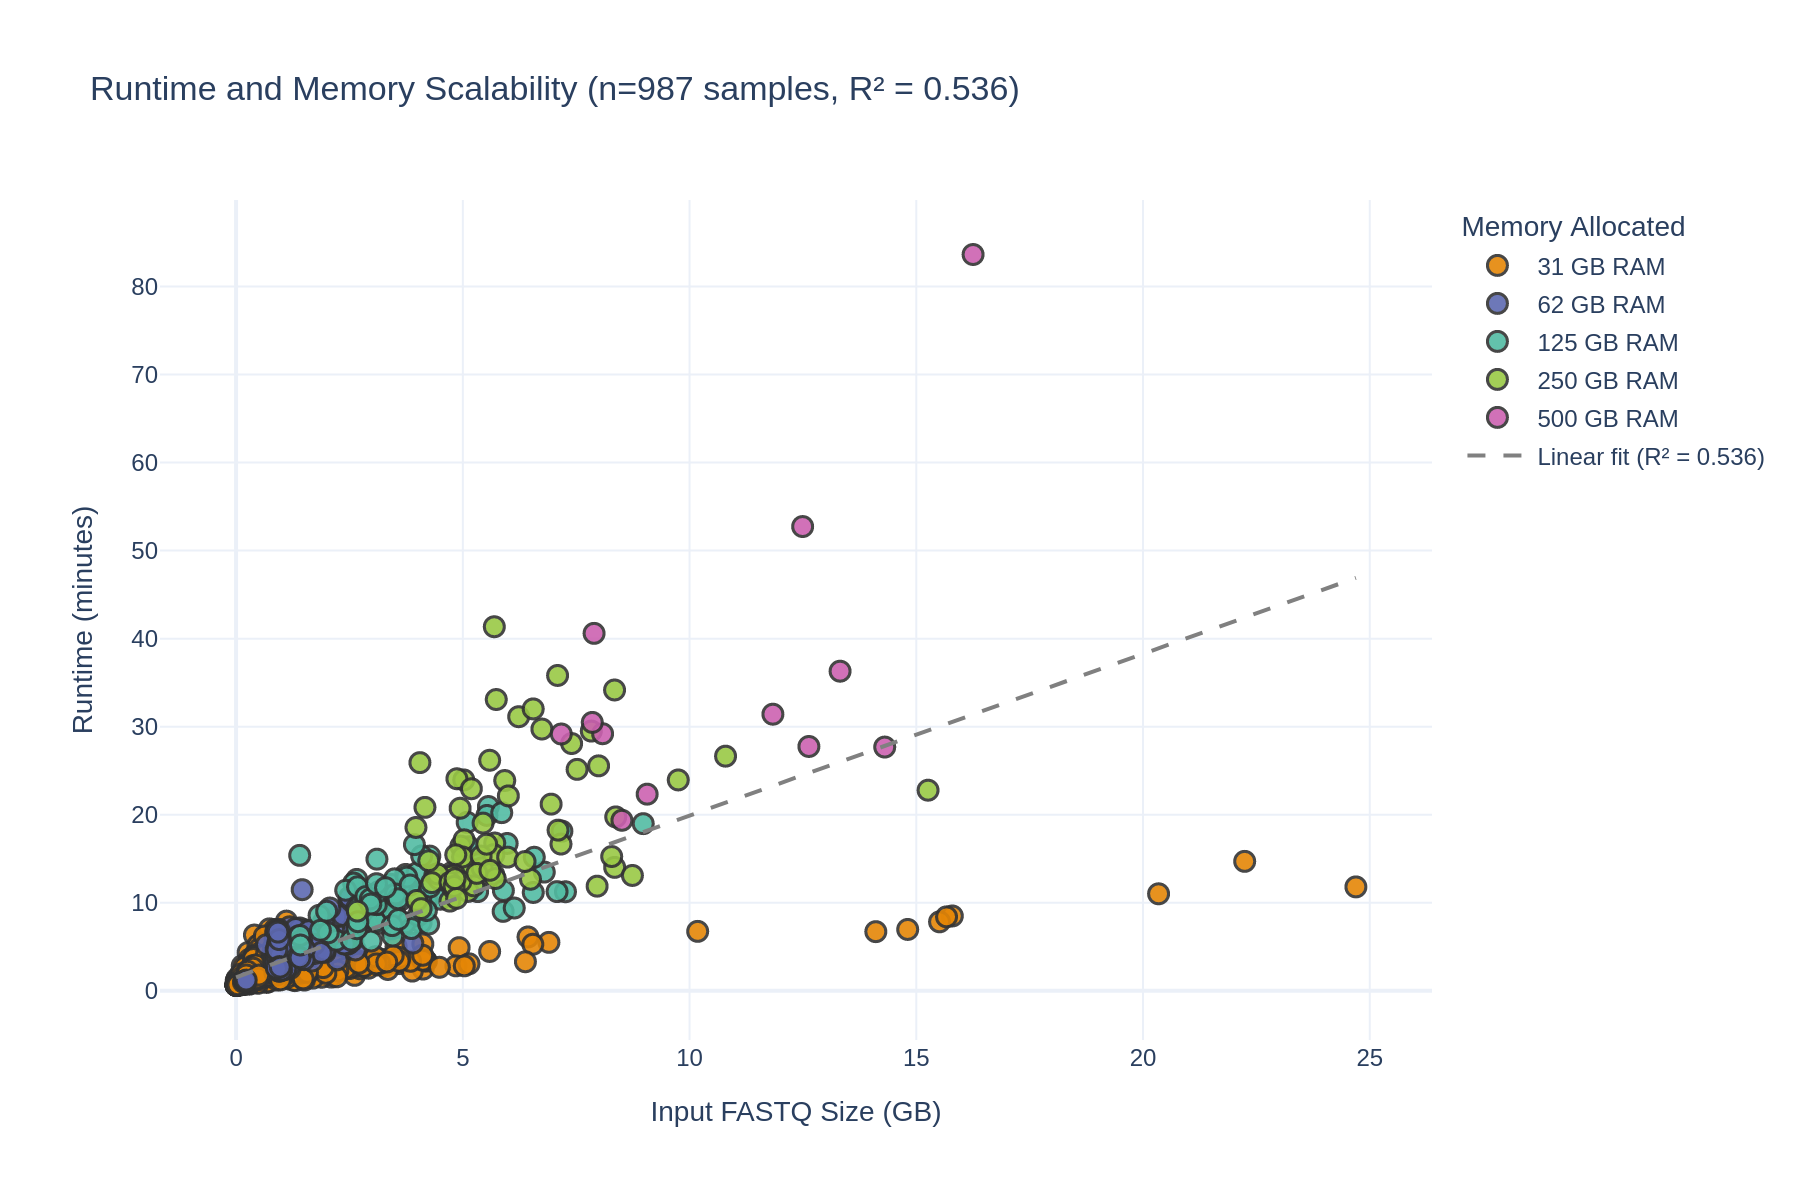
\includegraphics[width=0.95\textwidth]{sup_01_runtime_memory.png}
    \caption{\textbf{Runtime and memory scalability analysis.}
    Scatter plot showing the relationship between input FASTQ file size (GB) and runtime (minutes) 
    for DIANA predictions on the validation set. 
    Points are colored by RAM allocation (32-512 GB). 
    Linear regression fit (gray dashed line) shows a positive correlation (R² = 0.54), 
    with runtime averaging 1.84 minutes per GB of input data.
    All measurements obtained from validation set predictions on CPU (maestro cluster). 
    Each point represents one successfully processed sample.
    }
    \addcontentsline{toc}{subsection}{\protect\numberline{\thefigure}Runtime and memory scalability}
    \label{fig:sup_runtime_memory}
\end{figure}

% ===================================================================
% Supplementary Figure 2: Data Split Validation
% ===================================================================
\begin{figure}[p]
    \centering
    \subfloat[Sample Type Distribution]{%
        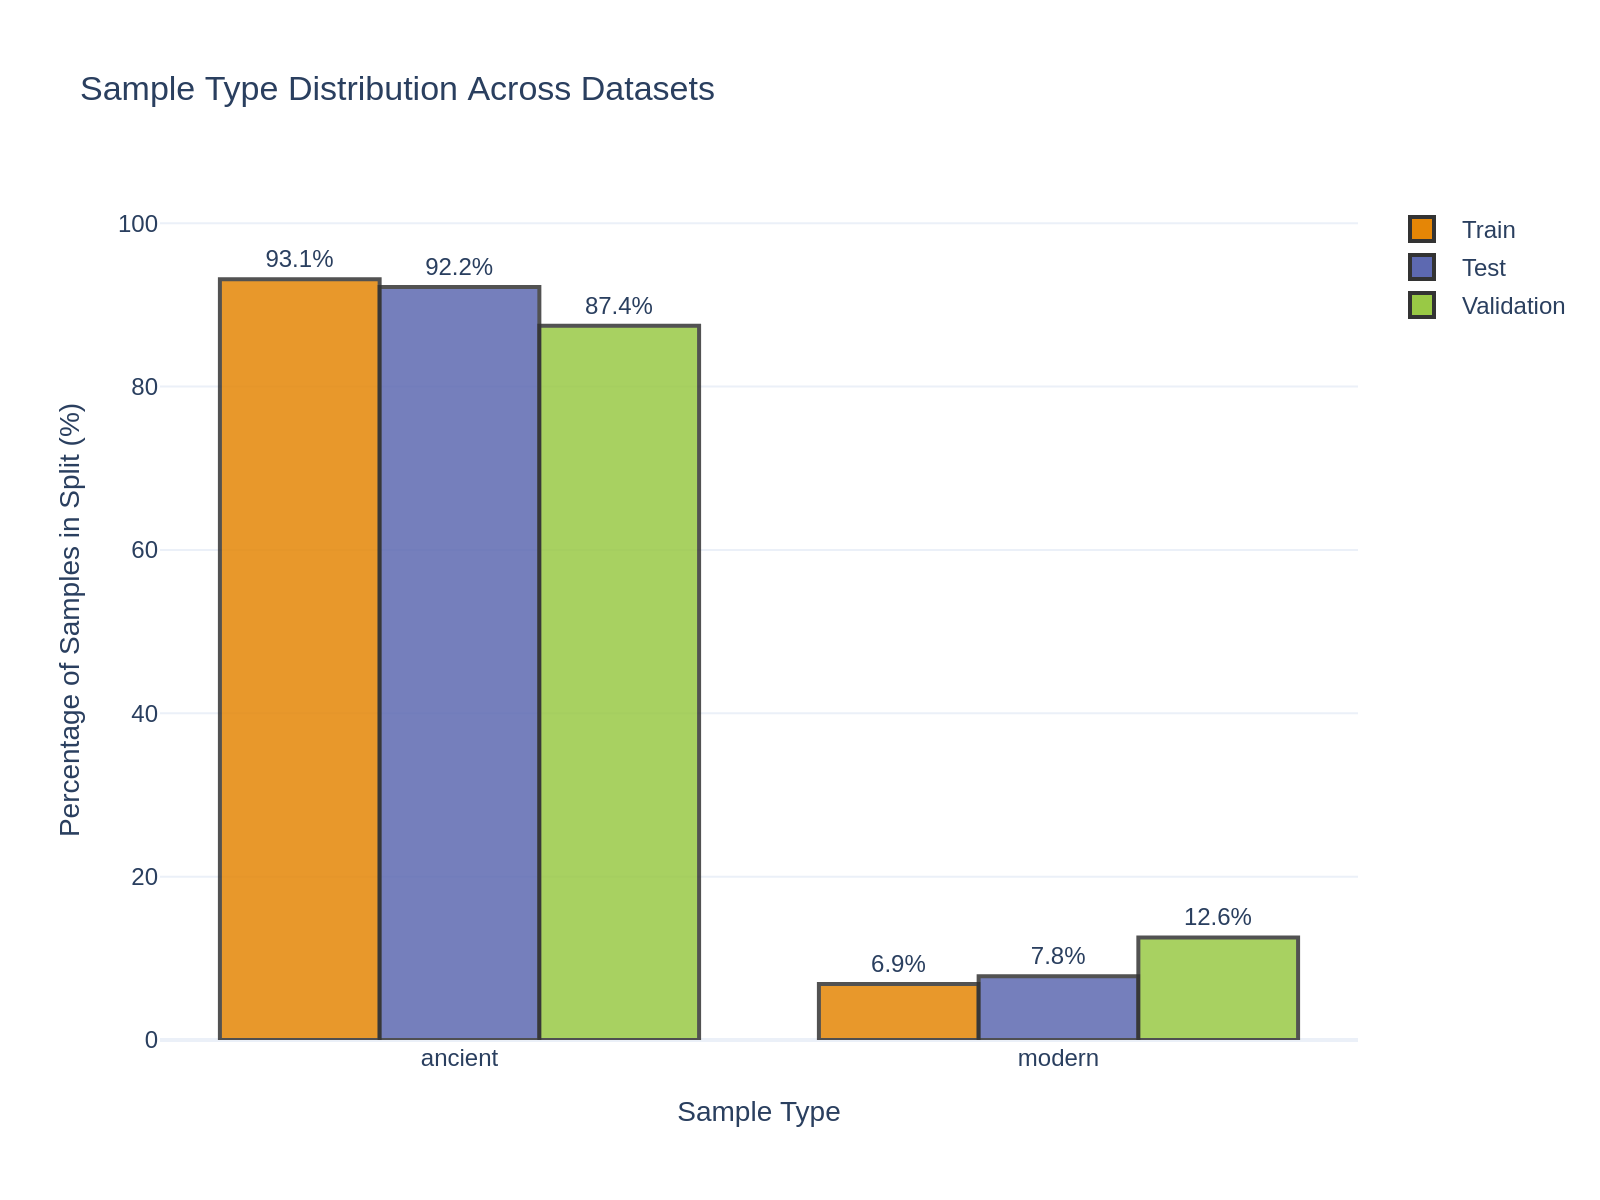
\includegraphics[width=0.48\textwidth]{sup_02_data_split_sample_type.png}%
    }
    \hfill
    \subfloat[Community Type Distribution]{%
        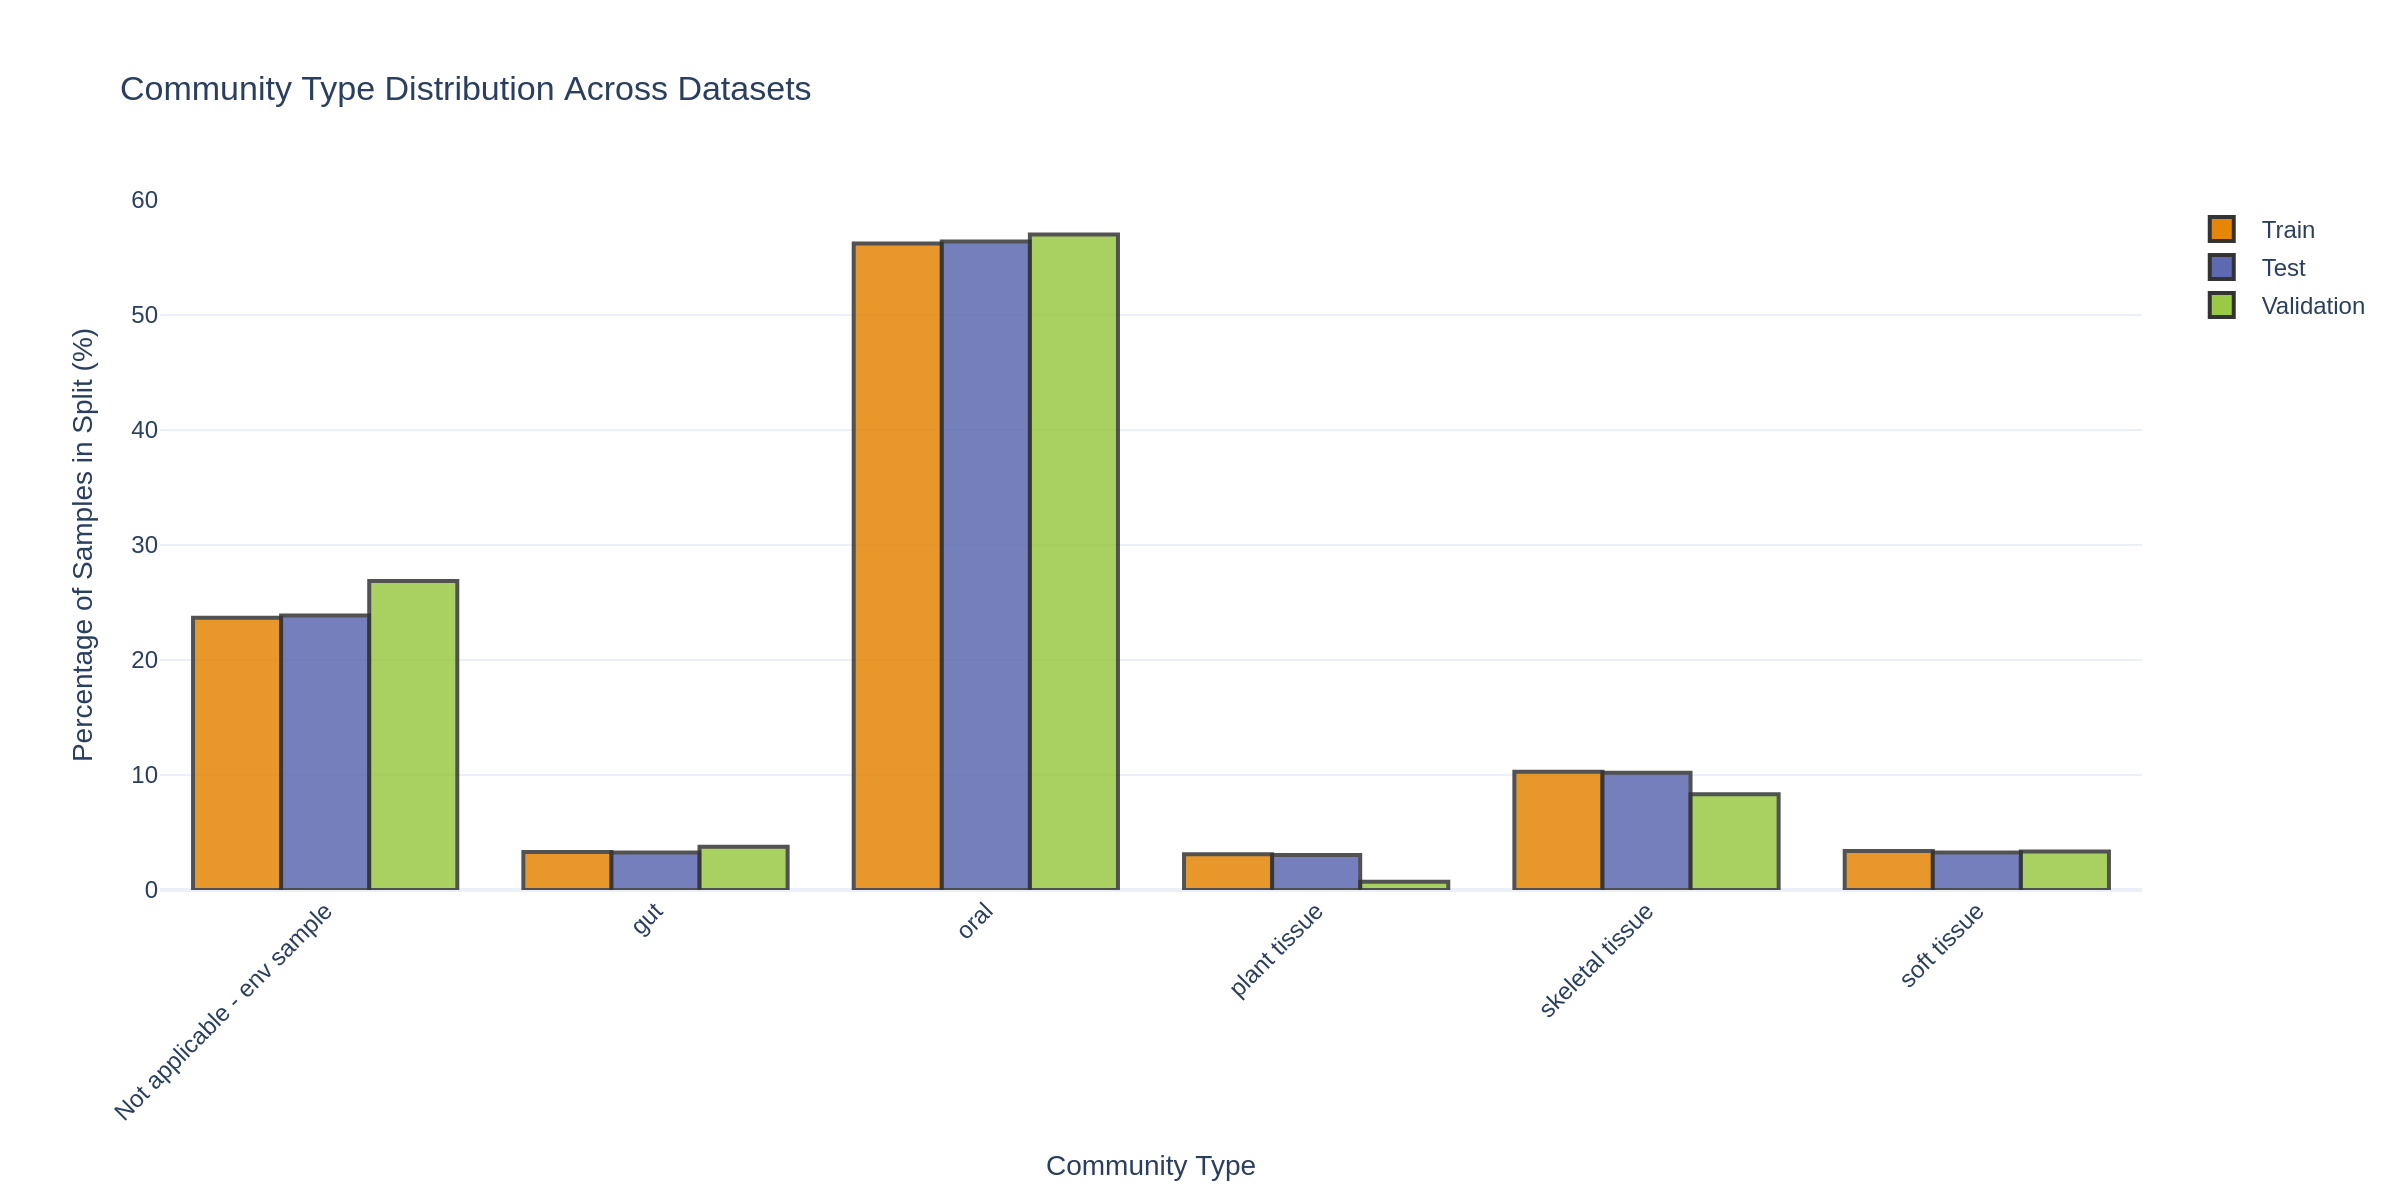
\includegraphics[width=0.48\textwidth]{sup_02_data_split_community_type.png}%
    }
    \\
    \subfloat[Material Distribution]{%
        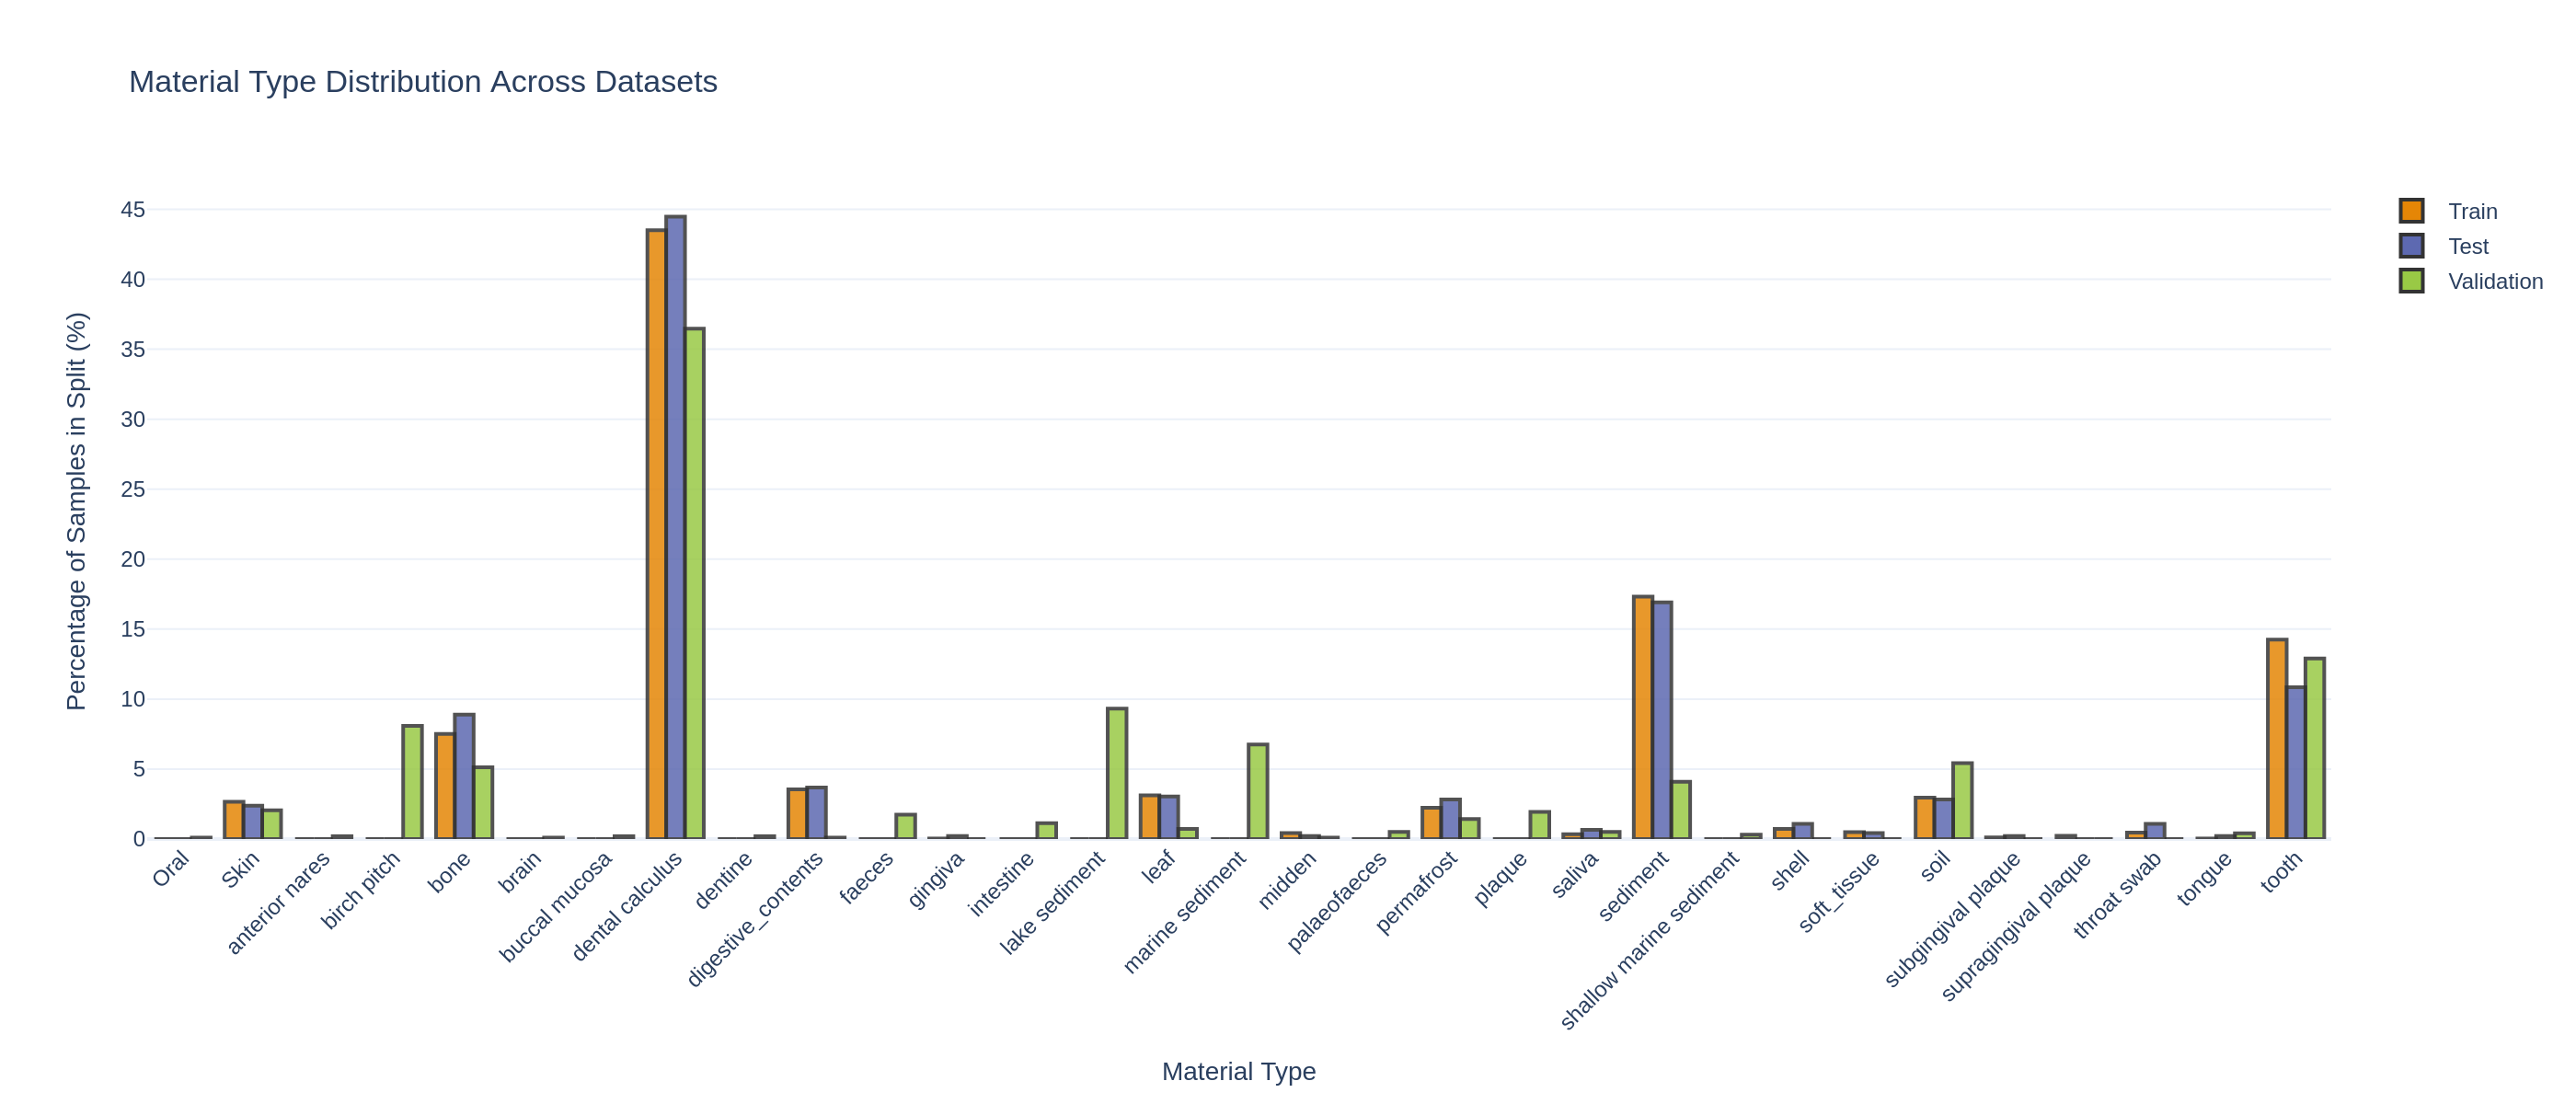
\includegraphics[width=0.48\textwidth]{sup_02_data_split_material.png}%
    }
    \hfill
    \subfloat[Project Distribution]{%
        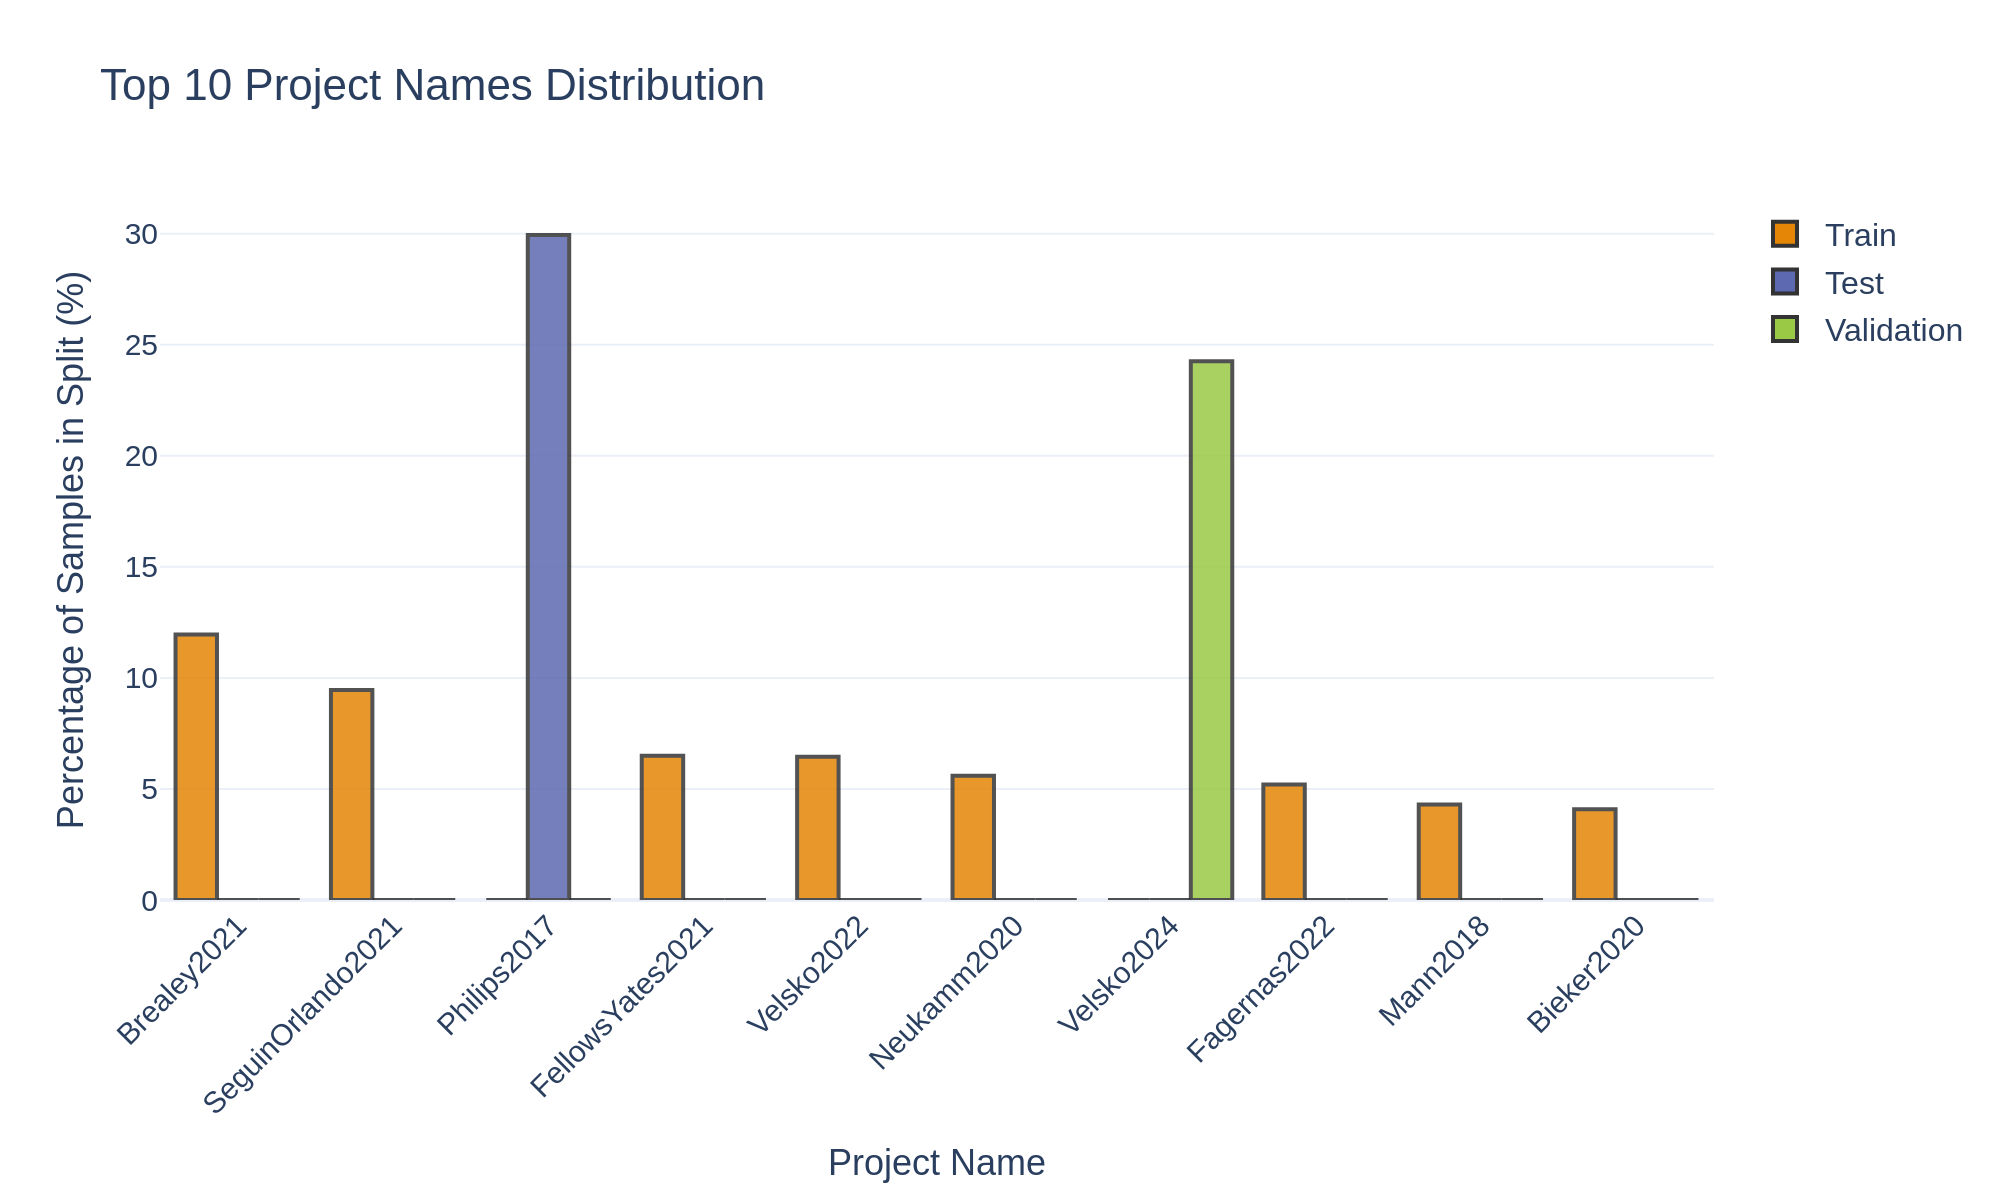
\includegraphics[width=0.48\textwidth]{sup_02_data_split_projects.png}%
    }
    \\
    \subfloat[Publication Year Distribution]{%
        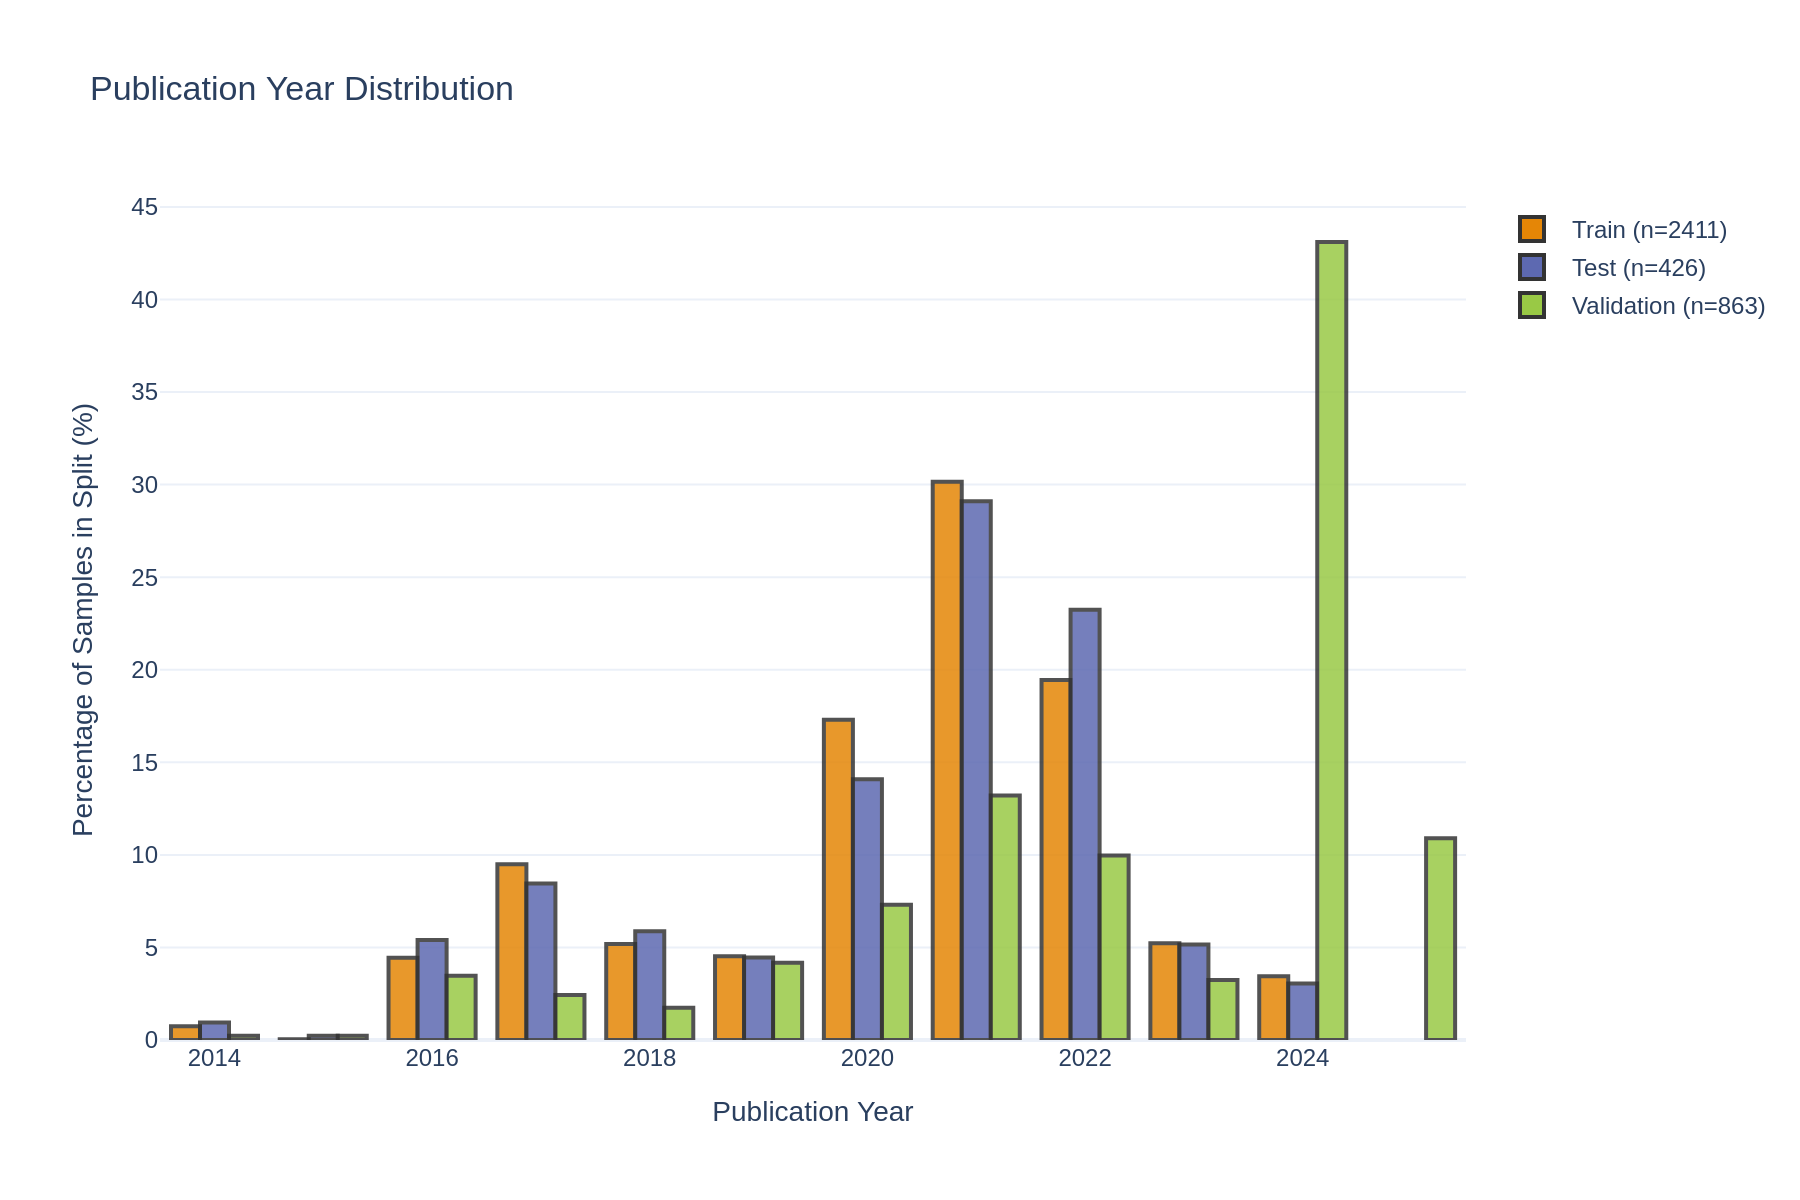
\includegraphics[width=0.48\textwidth]{sup_02_data_split_publication_year.png}%
    }
    \hfill
    \subfloat[File Size Distribution]{%
        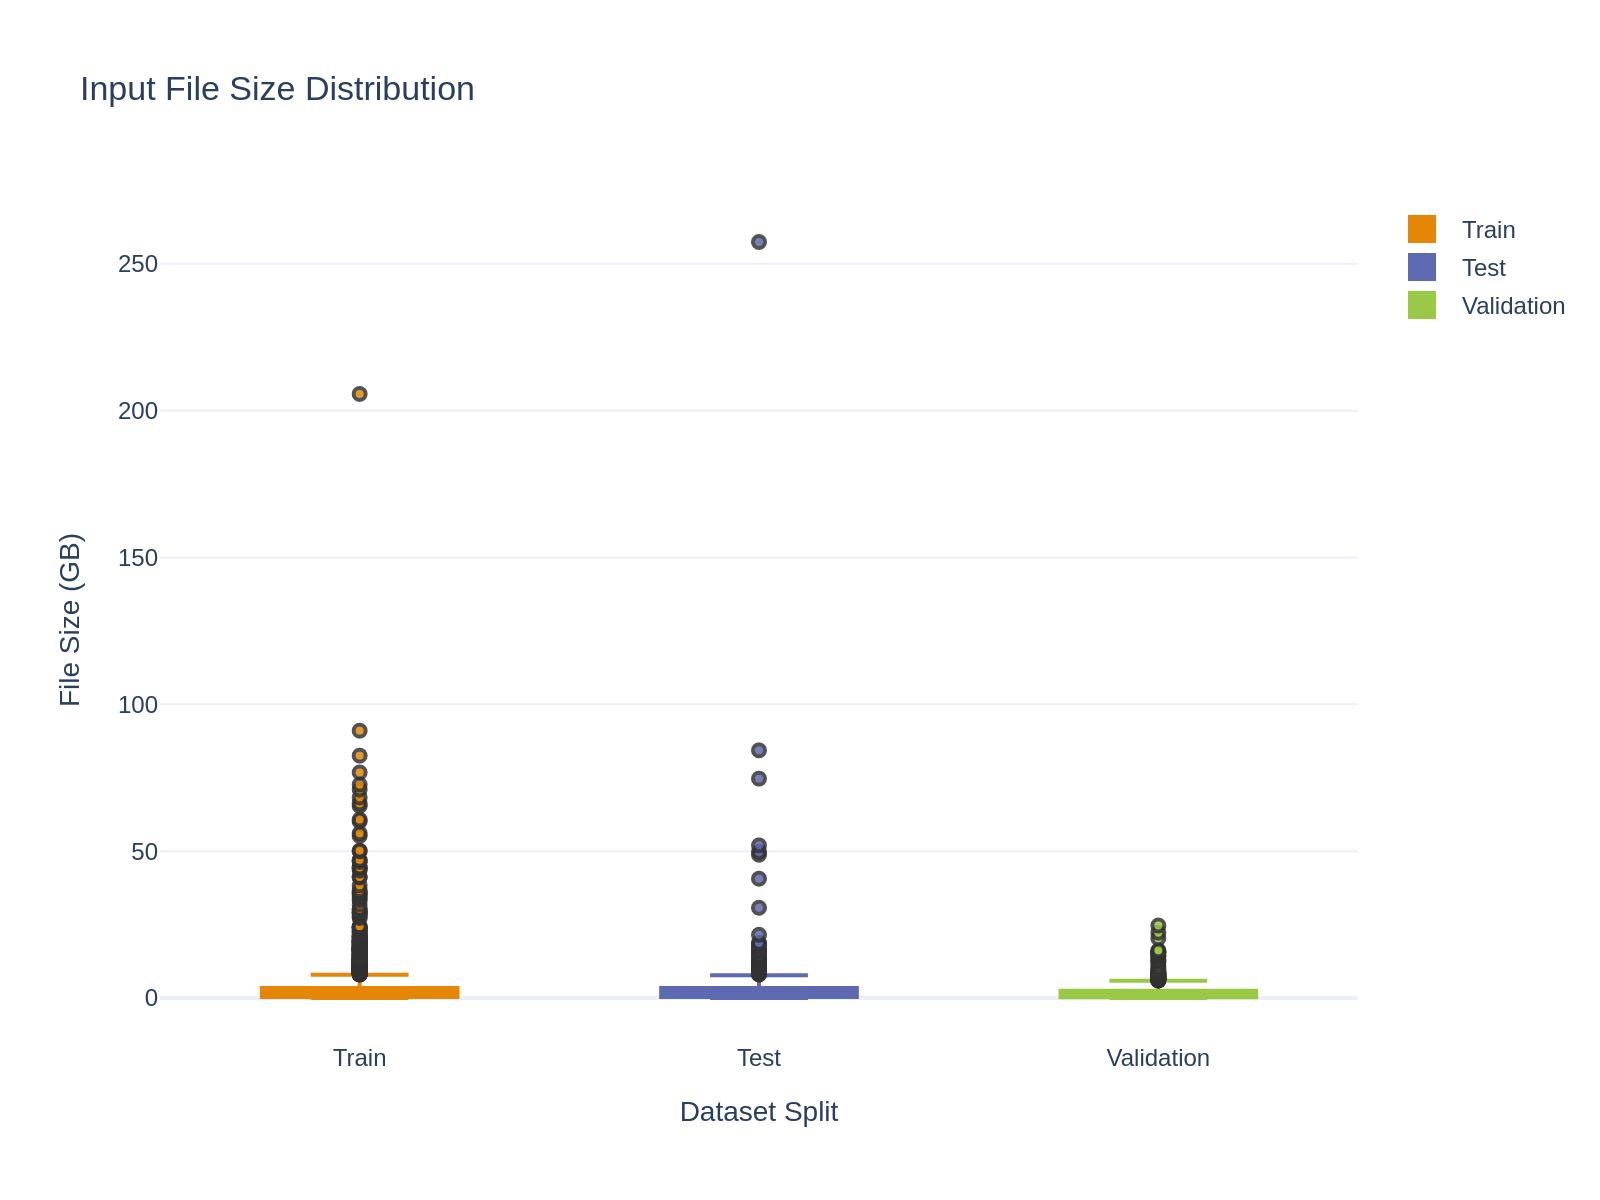
\includegraphics[width=0.48\textwidth]{sup_02_data_split_file_size.png}%
    }
    \caption{\textbf{Distribution comparison across train, test, and validation splits.}
    Bar plots showing the distribution of samples across different metadata categories for the training set (n=2,597), 
    held-out test set (n=461), and external validation set (n=1,029 total, 987 with successful predictions).
    (a) Sample type shows ancient (84\%) vs. modern (16\%) metagenome distribution, 
    with balanced representation across all splits.
    (b) Community type shows 6 tissue/environment categories in training, 
    with validation including 1 additional unseen class (Unknown).
    (c) Material shows 13 substrate types in training, 
    with validation including 7 additional unseen types (lake sediment, marine sediment, birch pitch, intestine, palaeofaeces, dentine, brain).
    (d) Project distribution across major sequencing initiatives (AncientMetagenomeDir studies and MGnify modern samples).
    (e) Publication year distribution demonstrates temporal coverage from 2014-2025.
    (f) File size distribution (log-scale, in MB) shows sequencing depth variability across datasets.
    The validation set's additional classes enable assessment of model generalization to unseen labels.
    }
    \addcontentsline{toc}{subsection}{\protect\numberline{\thefigure}Data split distribution comparison}
    \label{fig:sup_data_split}
\end{figure}

% ===================================================================
% Supplementary Figure 3: Geographic Distribution
% ===================================================================
\begin{figure}[p]
    \centering
    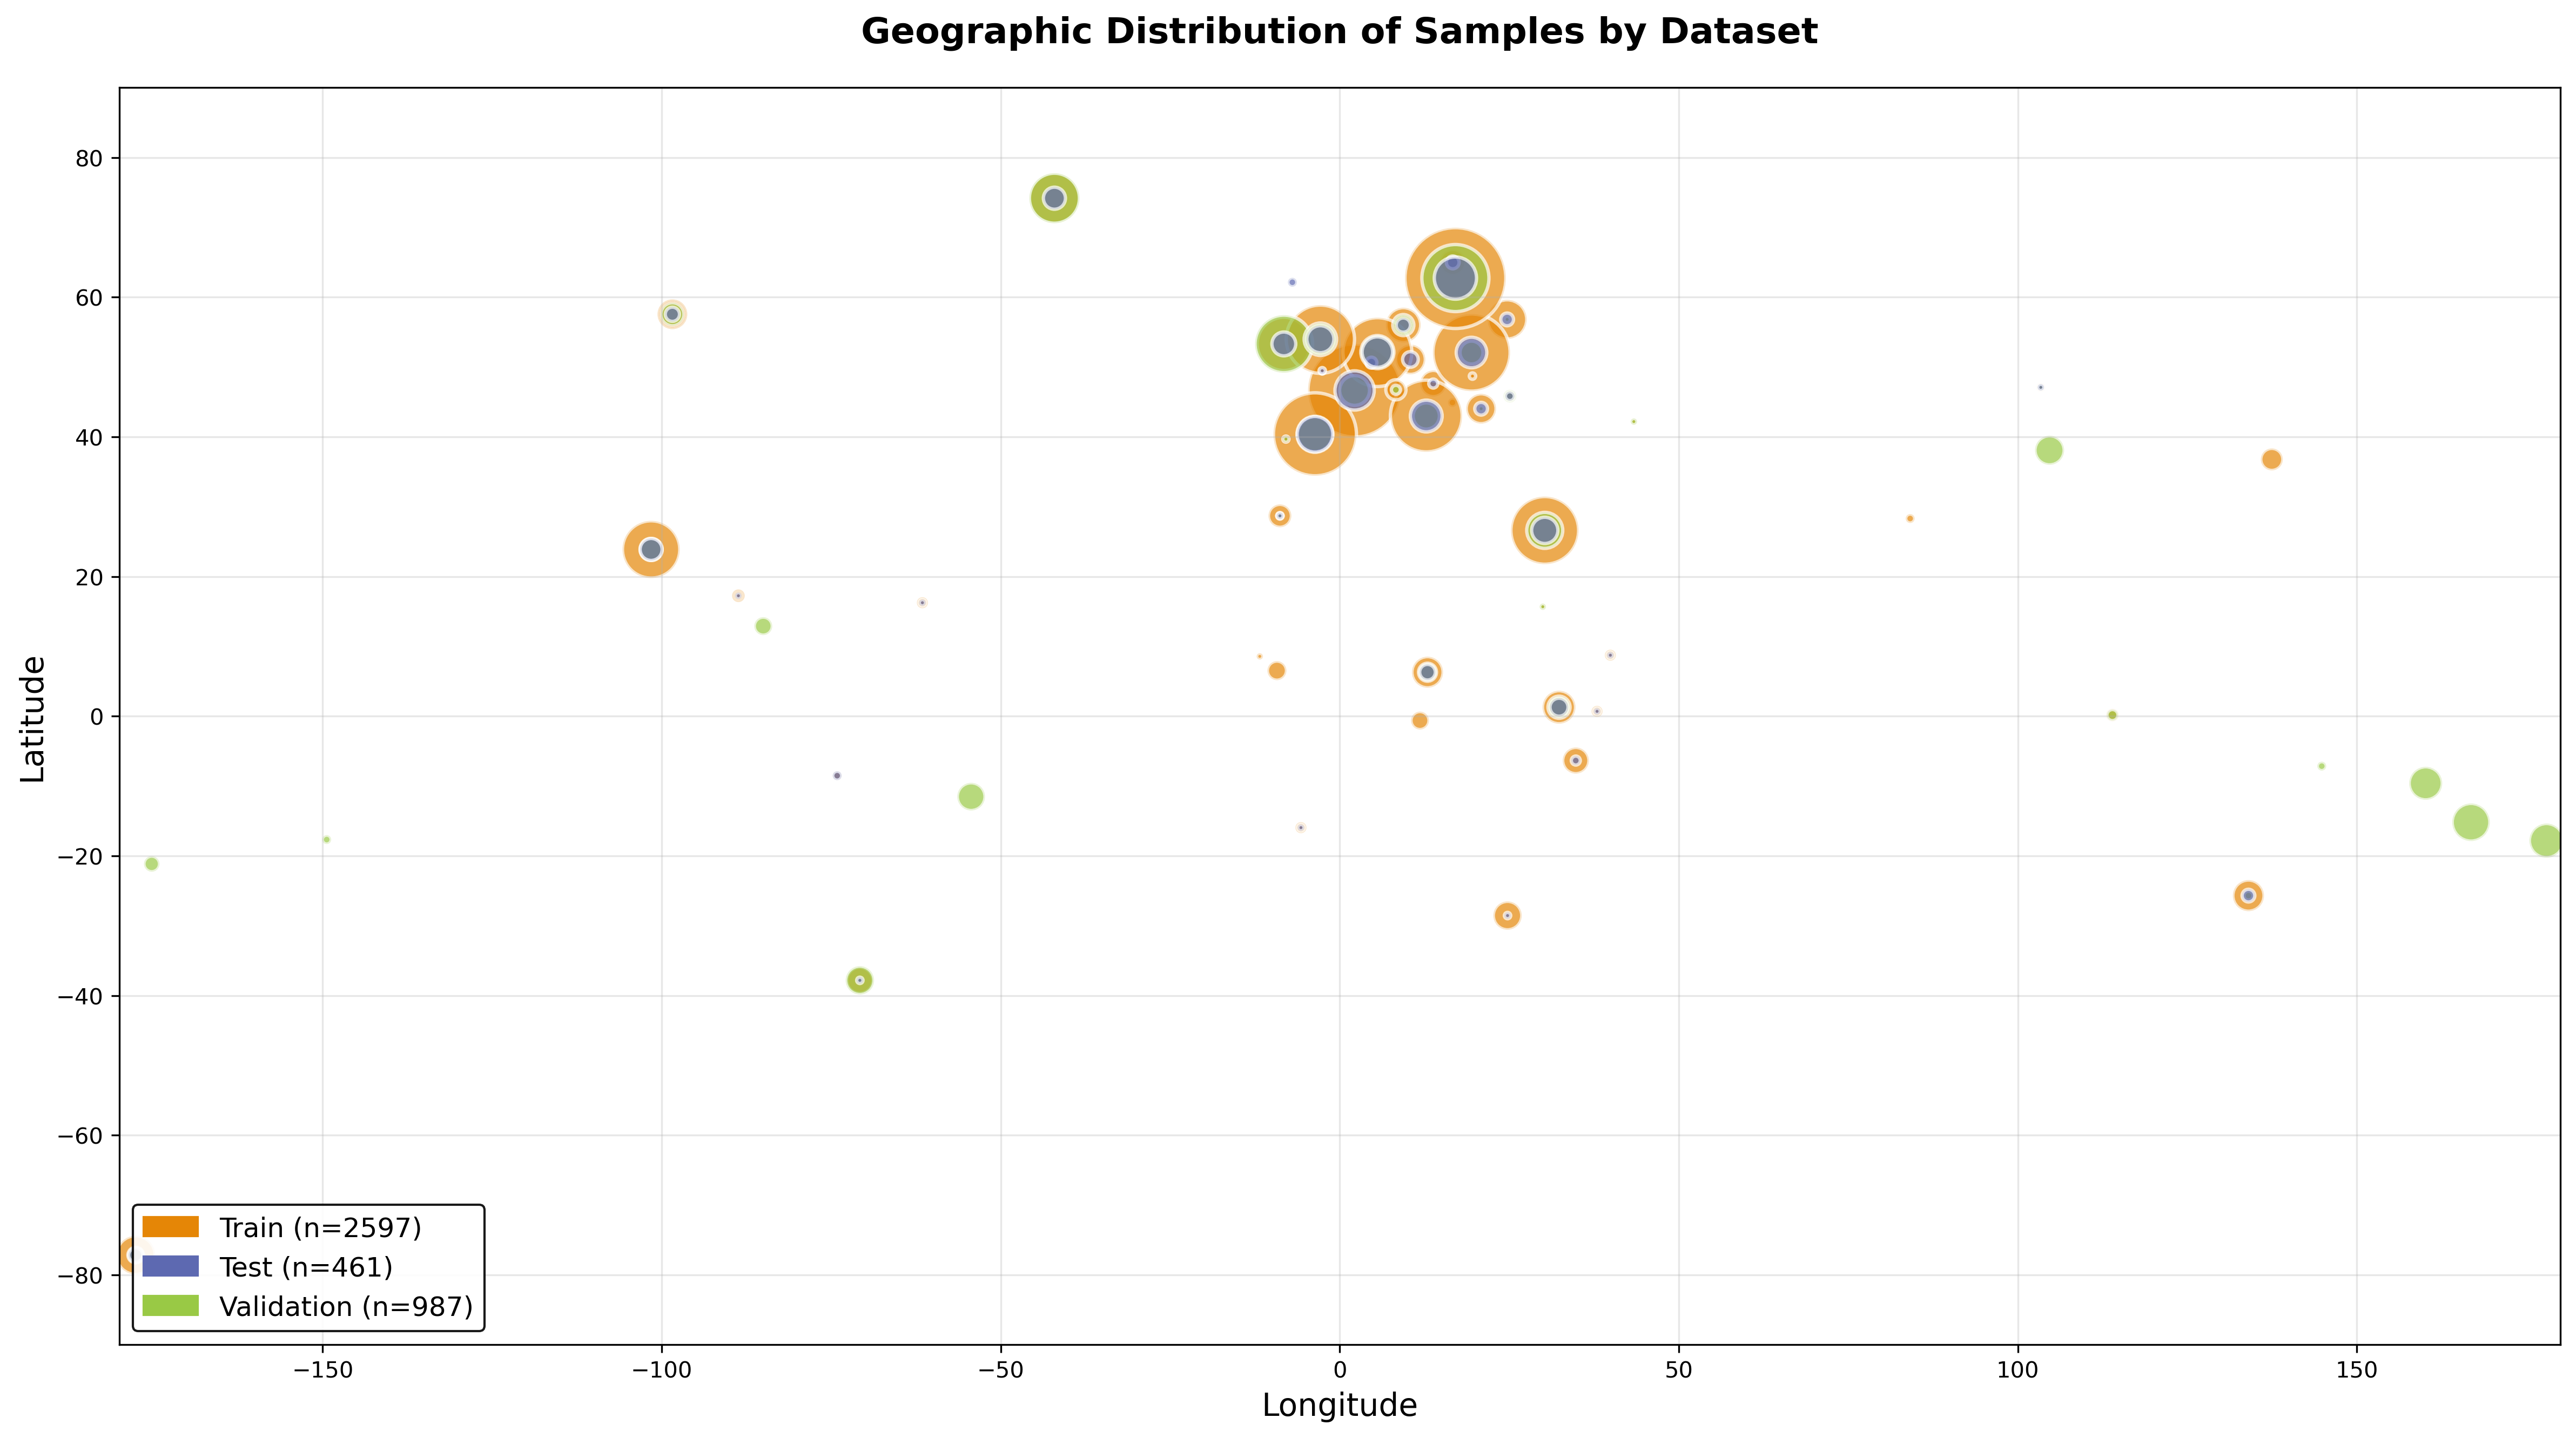
\includegraphics[width=0.95\textwidth]{sup_02_data_split_geographic.png}
    \caption{\textbf{Geographic distribution of samples by dataset.}
    World map showing global sampling coverage with points colored by dataset and sized by sample count. 
    Training (n=2,597) and test (n=461) samples predominantly from Europe and North America. 
    Validation samples (n=987) include broader geographic coverage from modern environmental samples via MGnify.
    }
    \addcontentsline{toc}{subsection}{\protect\numberline{\thefigure}Geographic distribution by dataset}
    \label{fig:sup_geographic}
\end{figure}

% ===================================================================
% Supplementary Figure 4: PCA Variance Explained (scree + cumulative)
% ===================================================================
\begin{figure}[p]
    \centering
    \subfloat[Variance explained per component]{%
        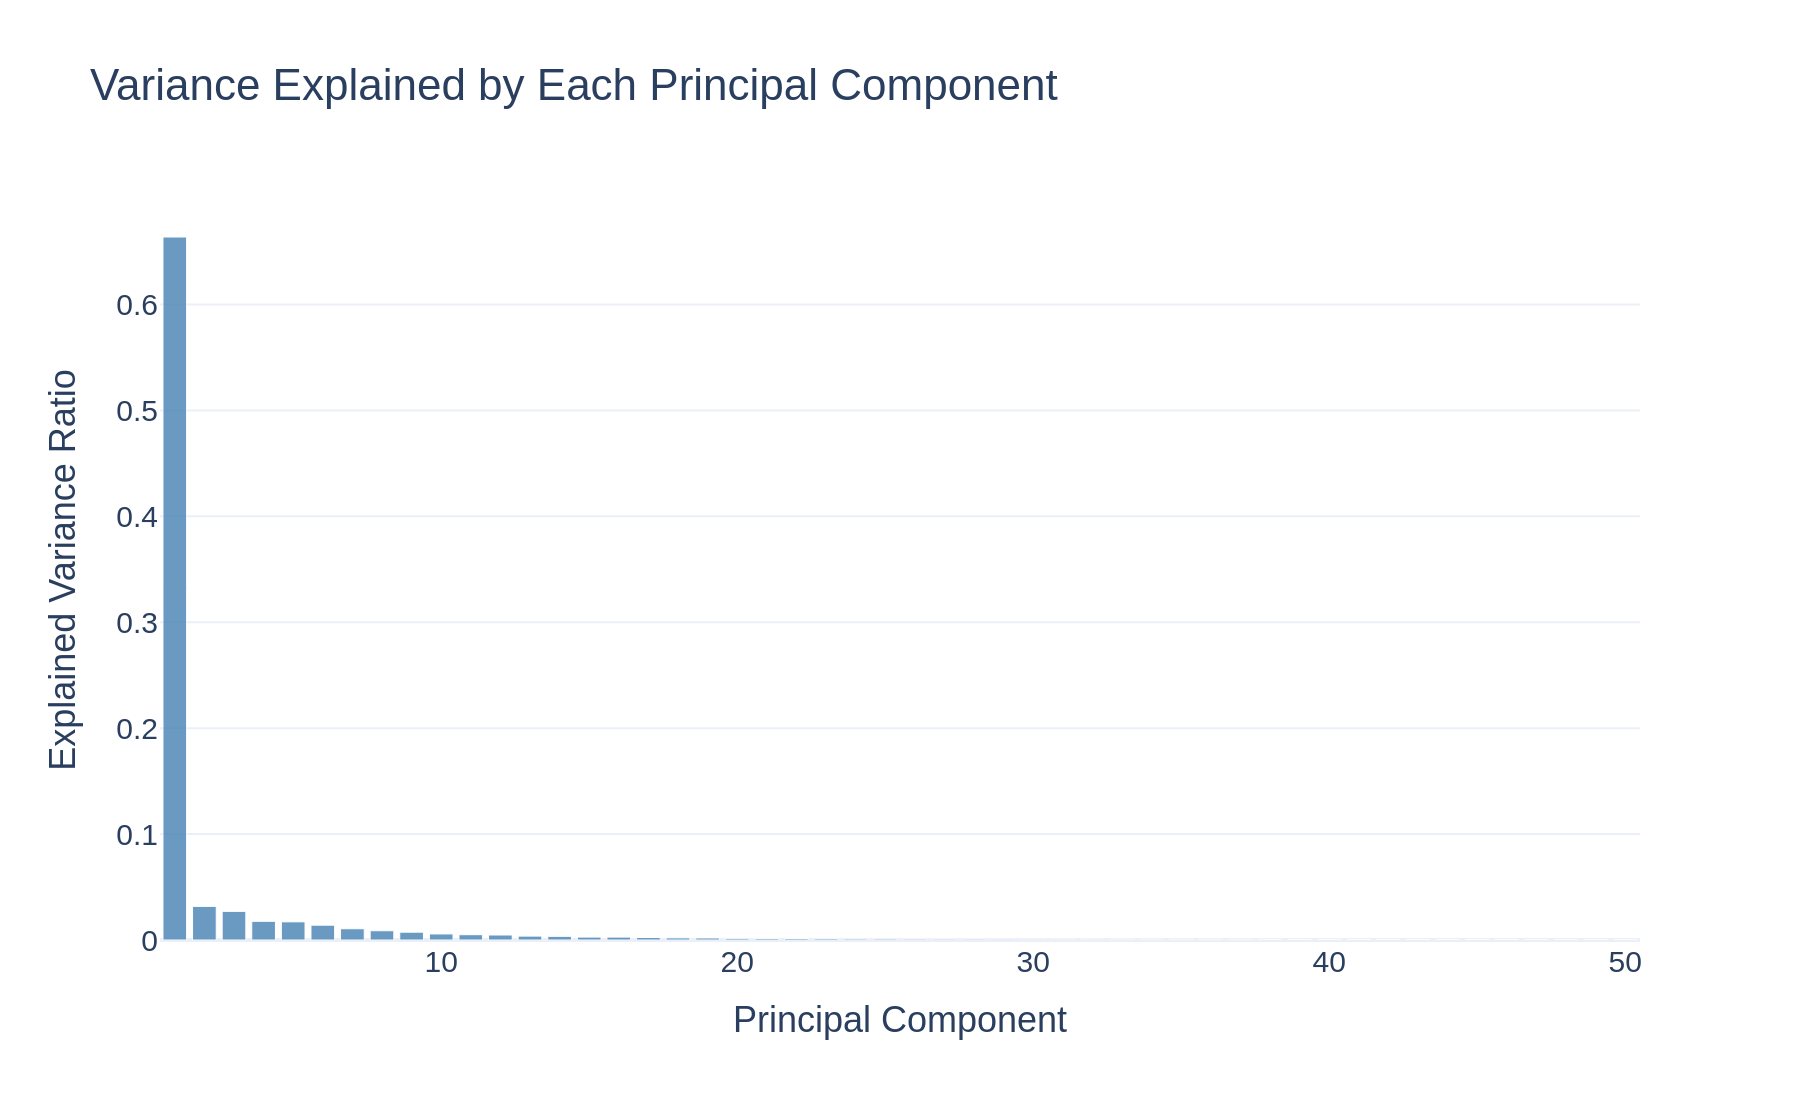
\includegraphics[width=0.82\textwidth]{sup_03_pca_scree.png}%
    }\\[1em]
    \subfloat[Cumulative variance explained]{%
        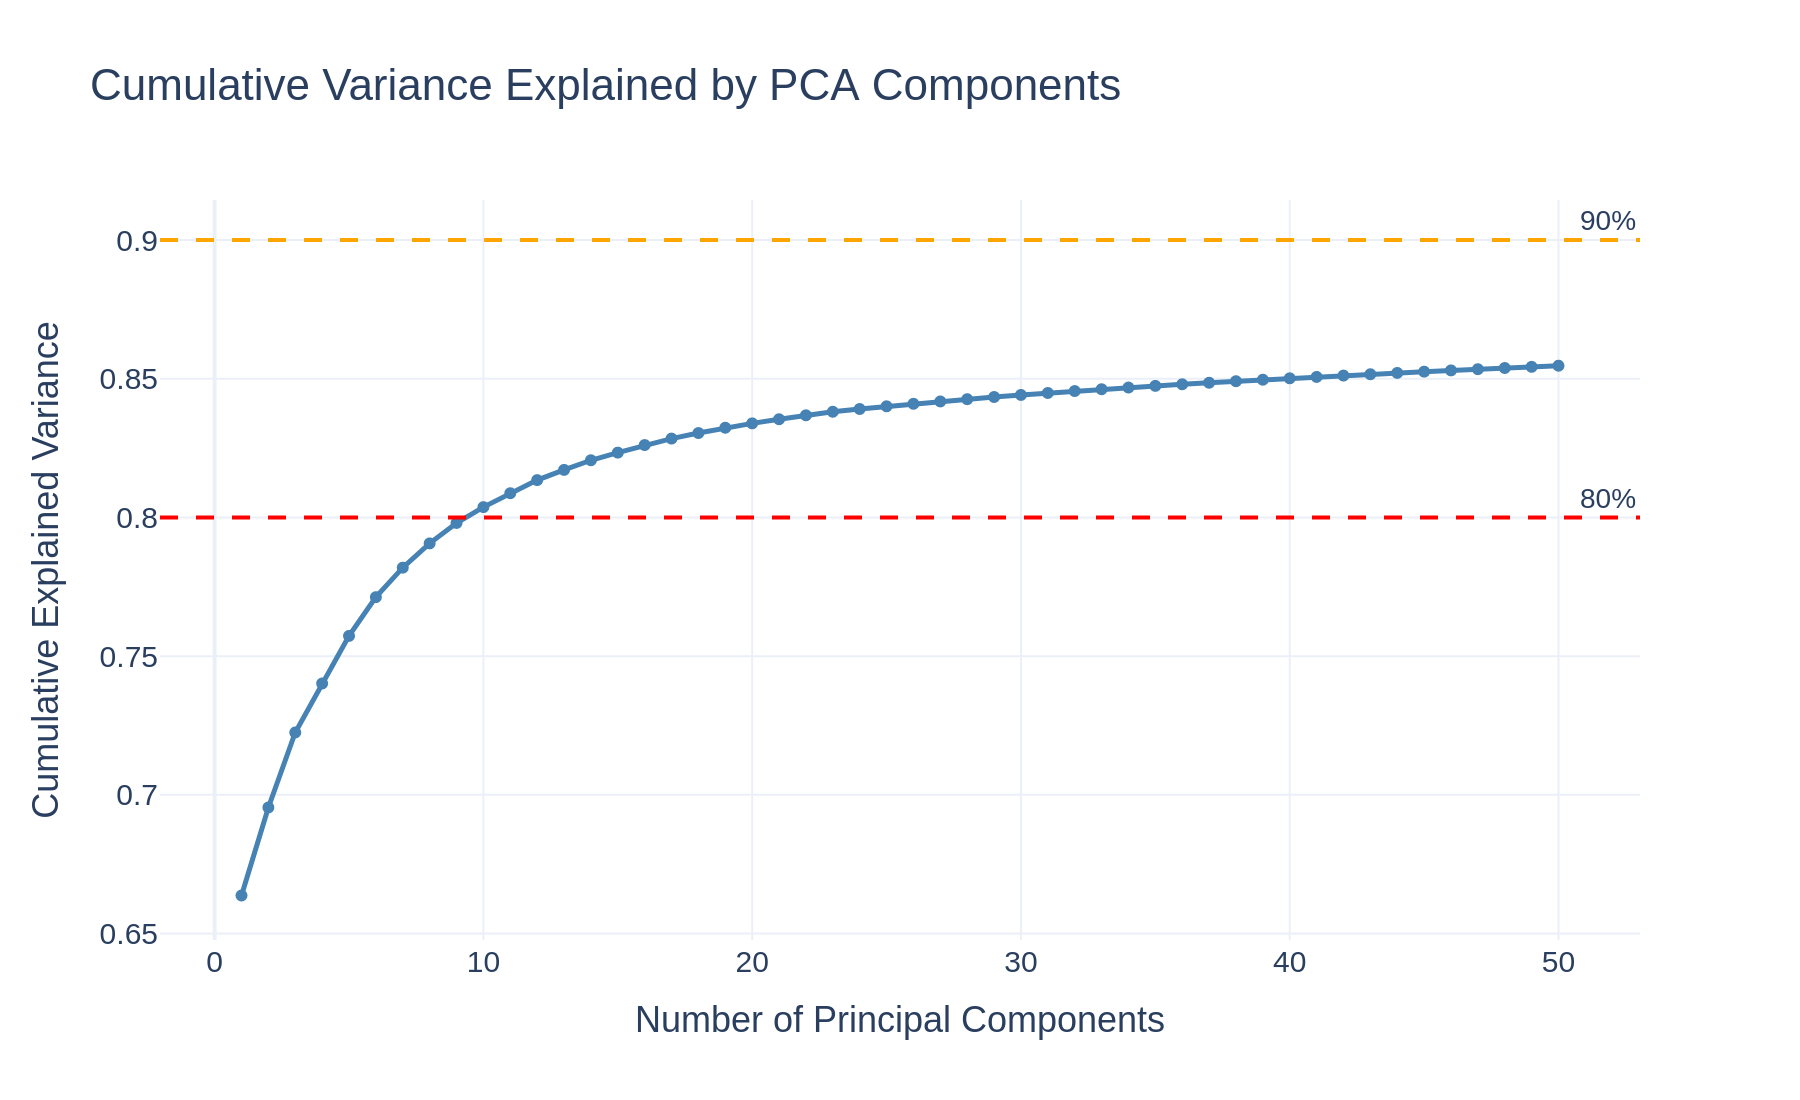
\includegraphics[width=0.82\textwidth]{sup_03_pca_cumulative_variance.png}%
    }
    \caption{\textbf{PCA variance explained by the unitig feature matrix.}
    PCA computed on training and test samples (n=3,058: 2,597 train + 461 test)
    using 107,480 unitig features.
    \textbf{(a)} Variance explained by each of the first 50 principal components.
    PC1 alone accounts for 66.4\% of total variance, showing a dominant first component
    with a sharp drop to PC2 (3.2\%) and a gradual, long tail thereafter.
    \textbf{(b)} Cumulative variance explained.
    The first two components together capture approximately 70\% of total variance;
    the 80\% threshold is reached at \textasciitilde{}10 components, and
    90\% is not reached even at 50 components (\textasciitilde{}86\%).
    Although PC1 captures substantial variance, the remaining variance is spread
    across many components, highlighting why linear dimensionality reduction alone is
    insufficient for this classification task and motivates deep neural networks.
    }
    \addcontentsline{toc}{subsection}{\protect\numberline{\thefigure}PCA variance explained}
    \label{fig:sup_pca_scree}
\end{figure}

\clearpage

% ===================================================================
% Supplementary Figure 5: PCA Projections by Task
% ===================================================================
\begin{figure}[p]
    \centering
    \subfloat[Sample Type]{%
        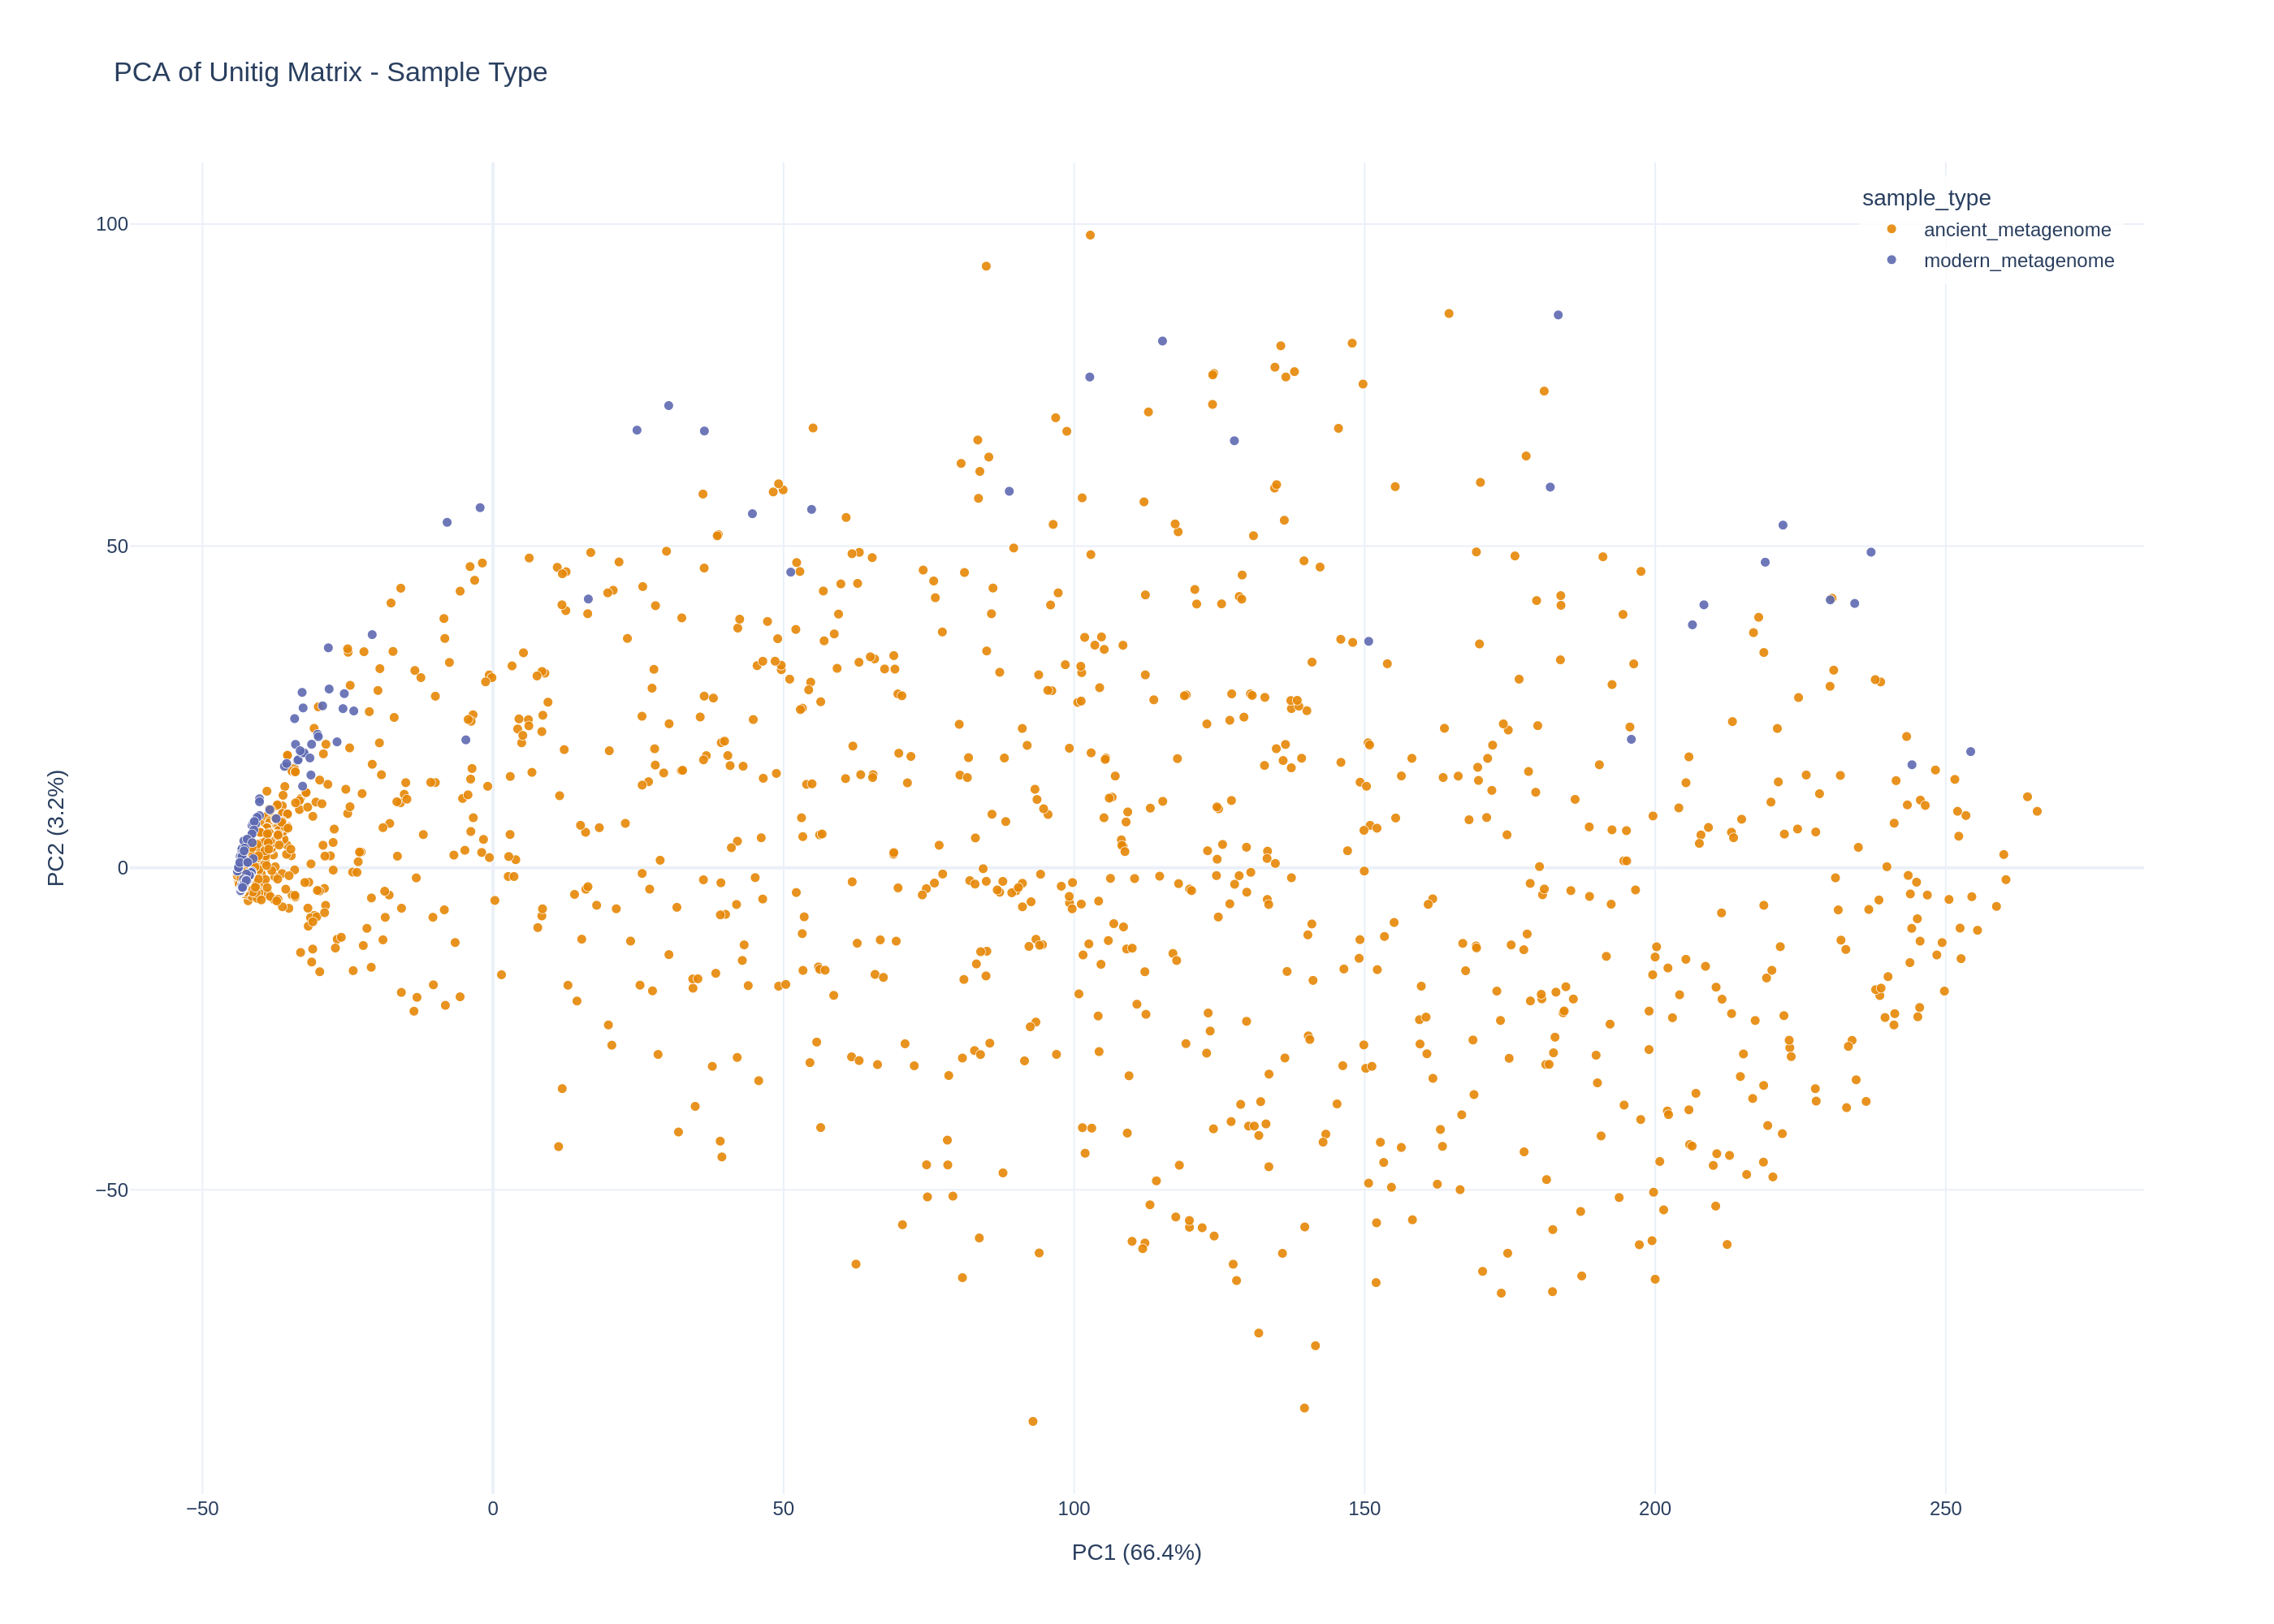
\includegraphics[width=0.48\textwidth]{sup_03_pca_sample_type.png}%
    }
    \hfill
    \subfloat[Community Type]{%
        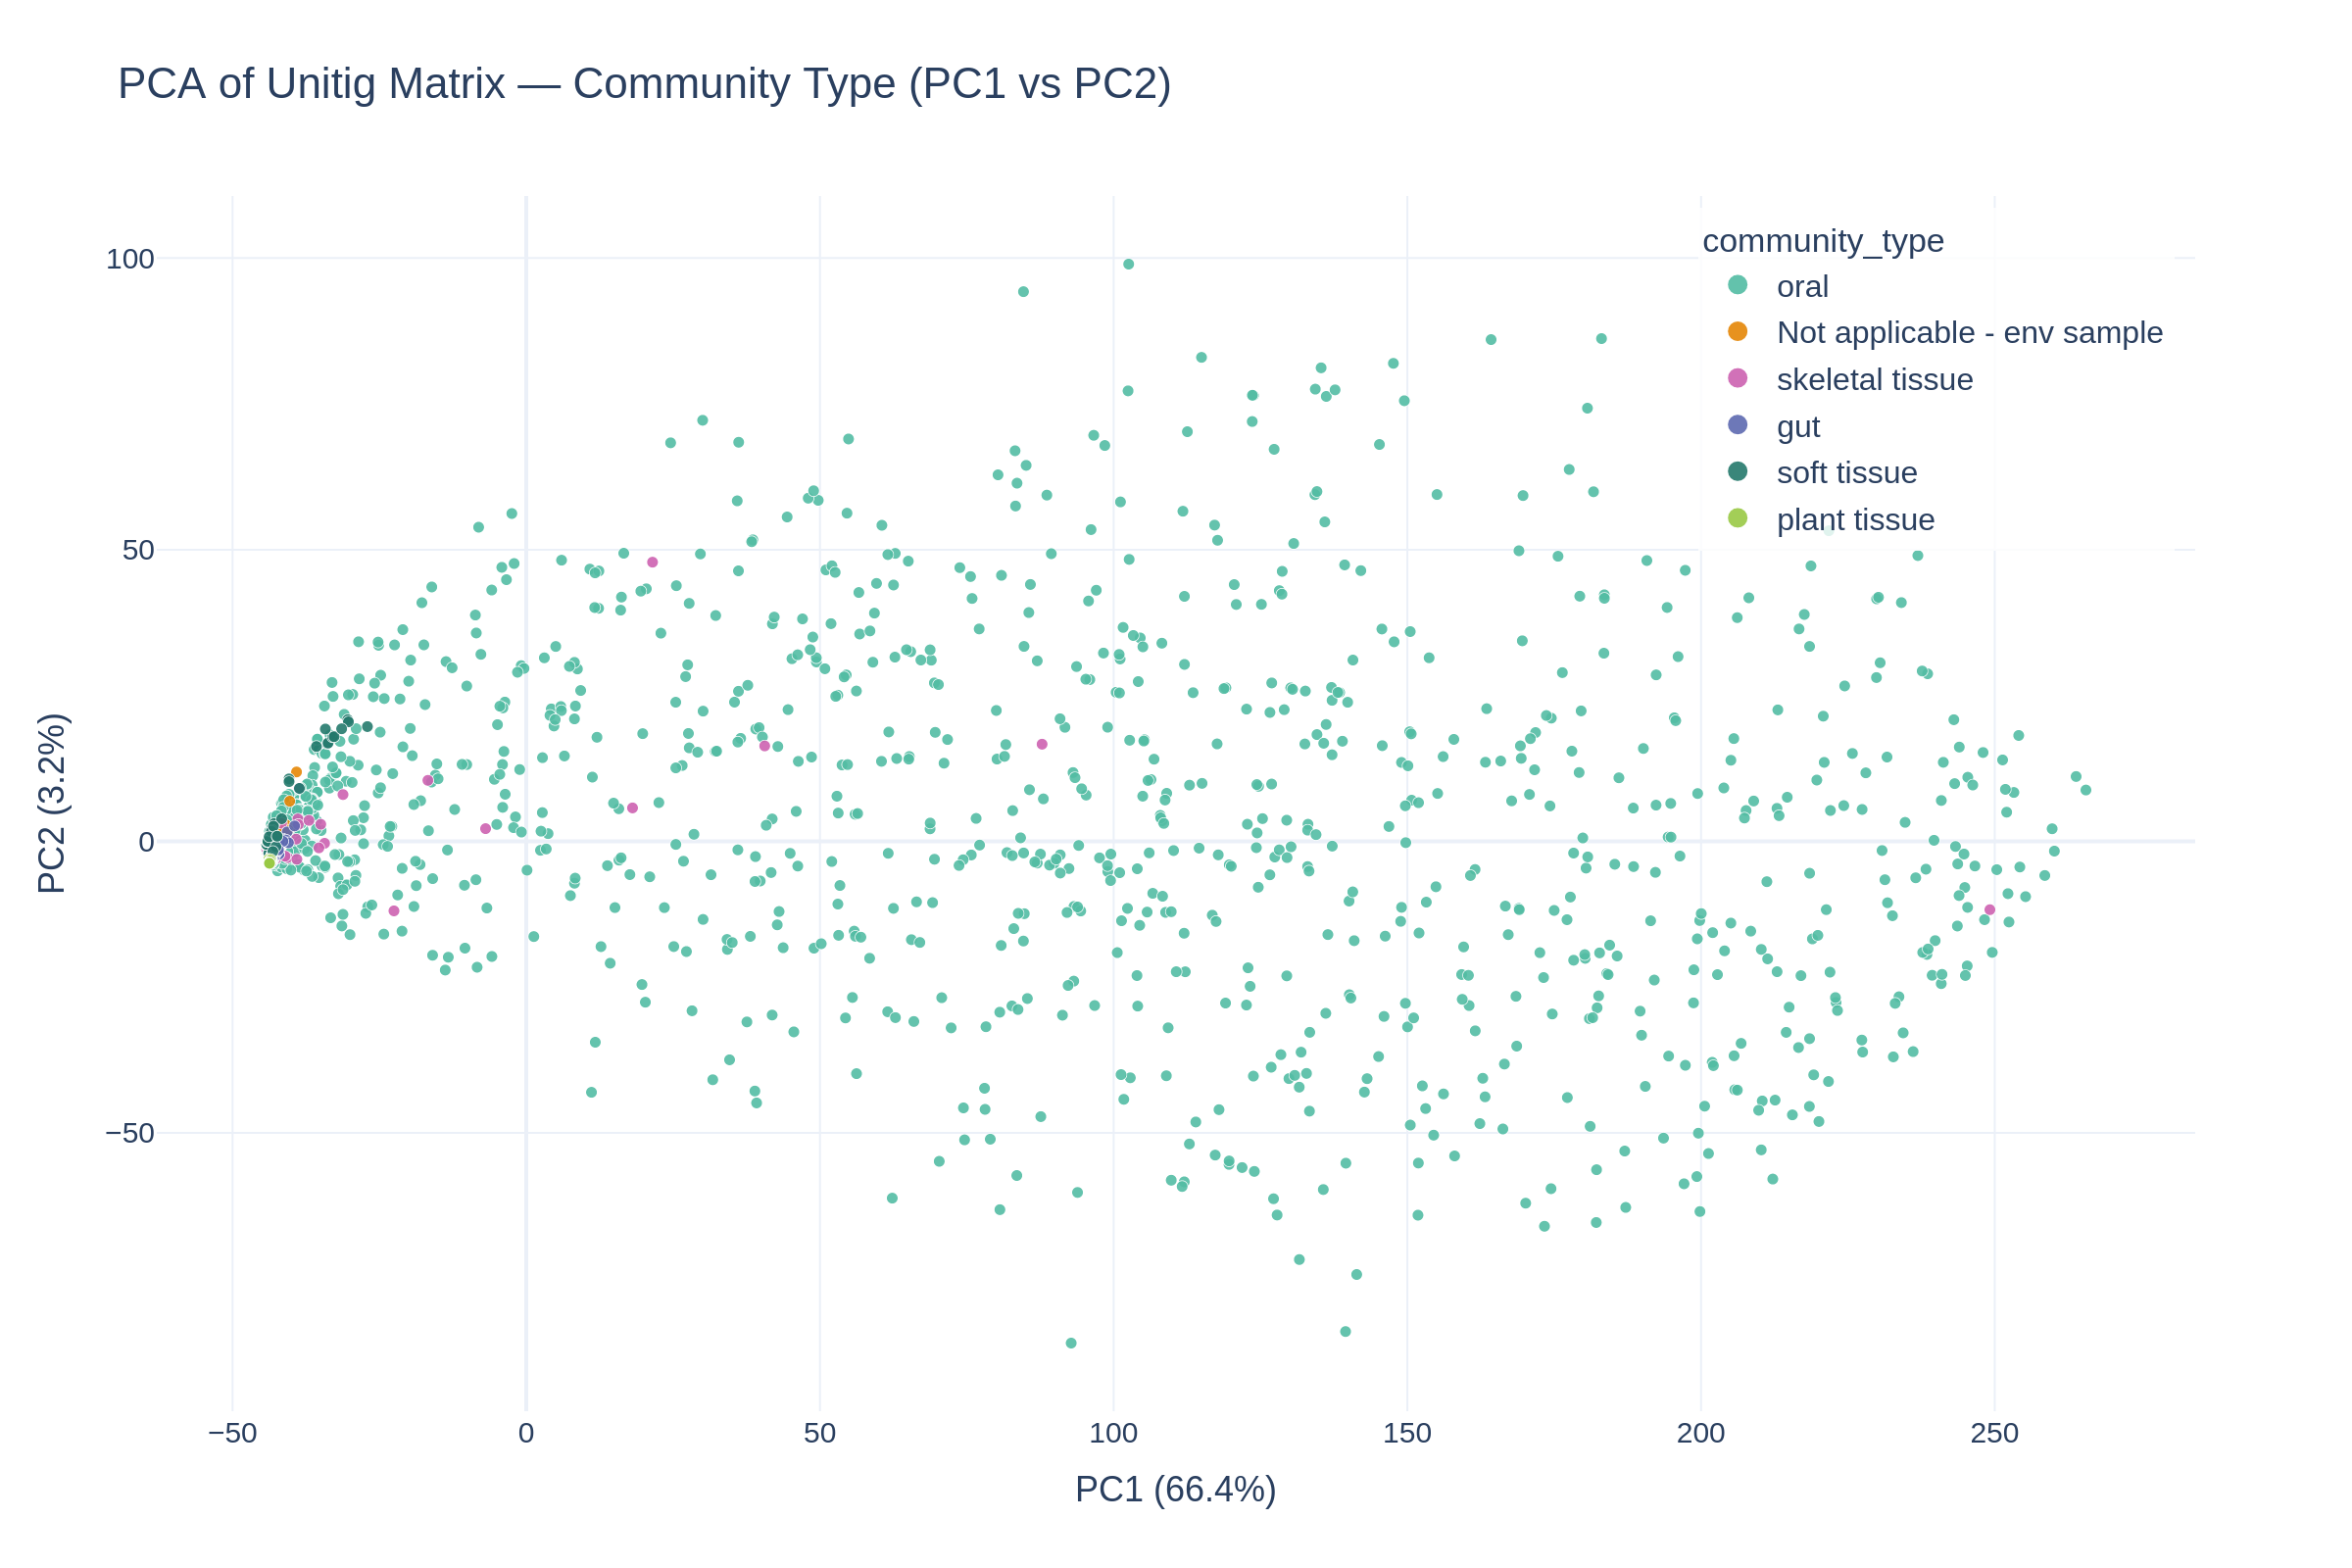
\includegraphics[width=0.48\textwidth]{sup_03_pca_community_type.png}%
    }
    \\
    \subfloat[Sample Host]{%
        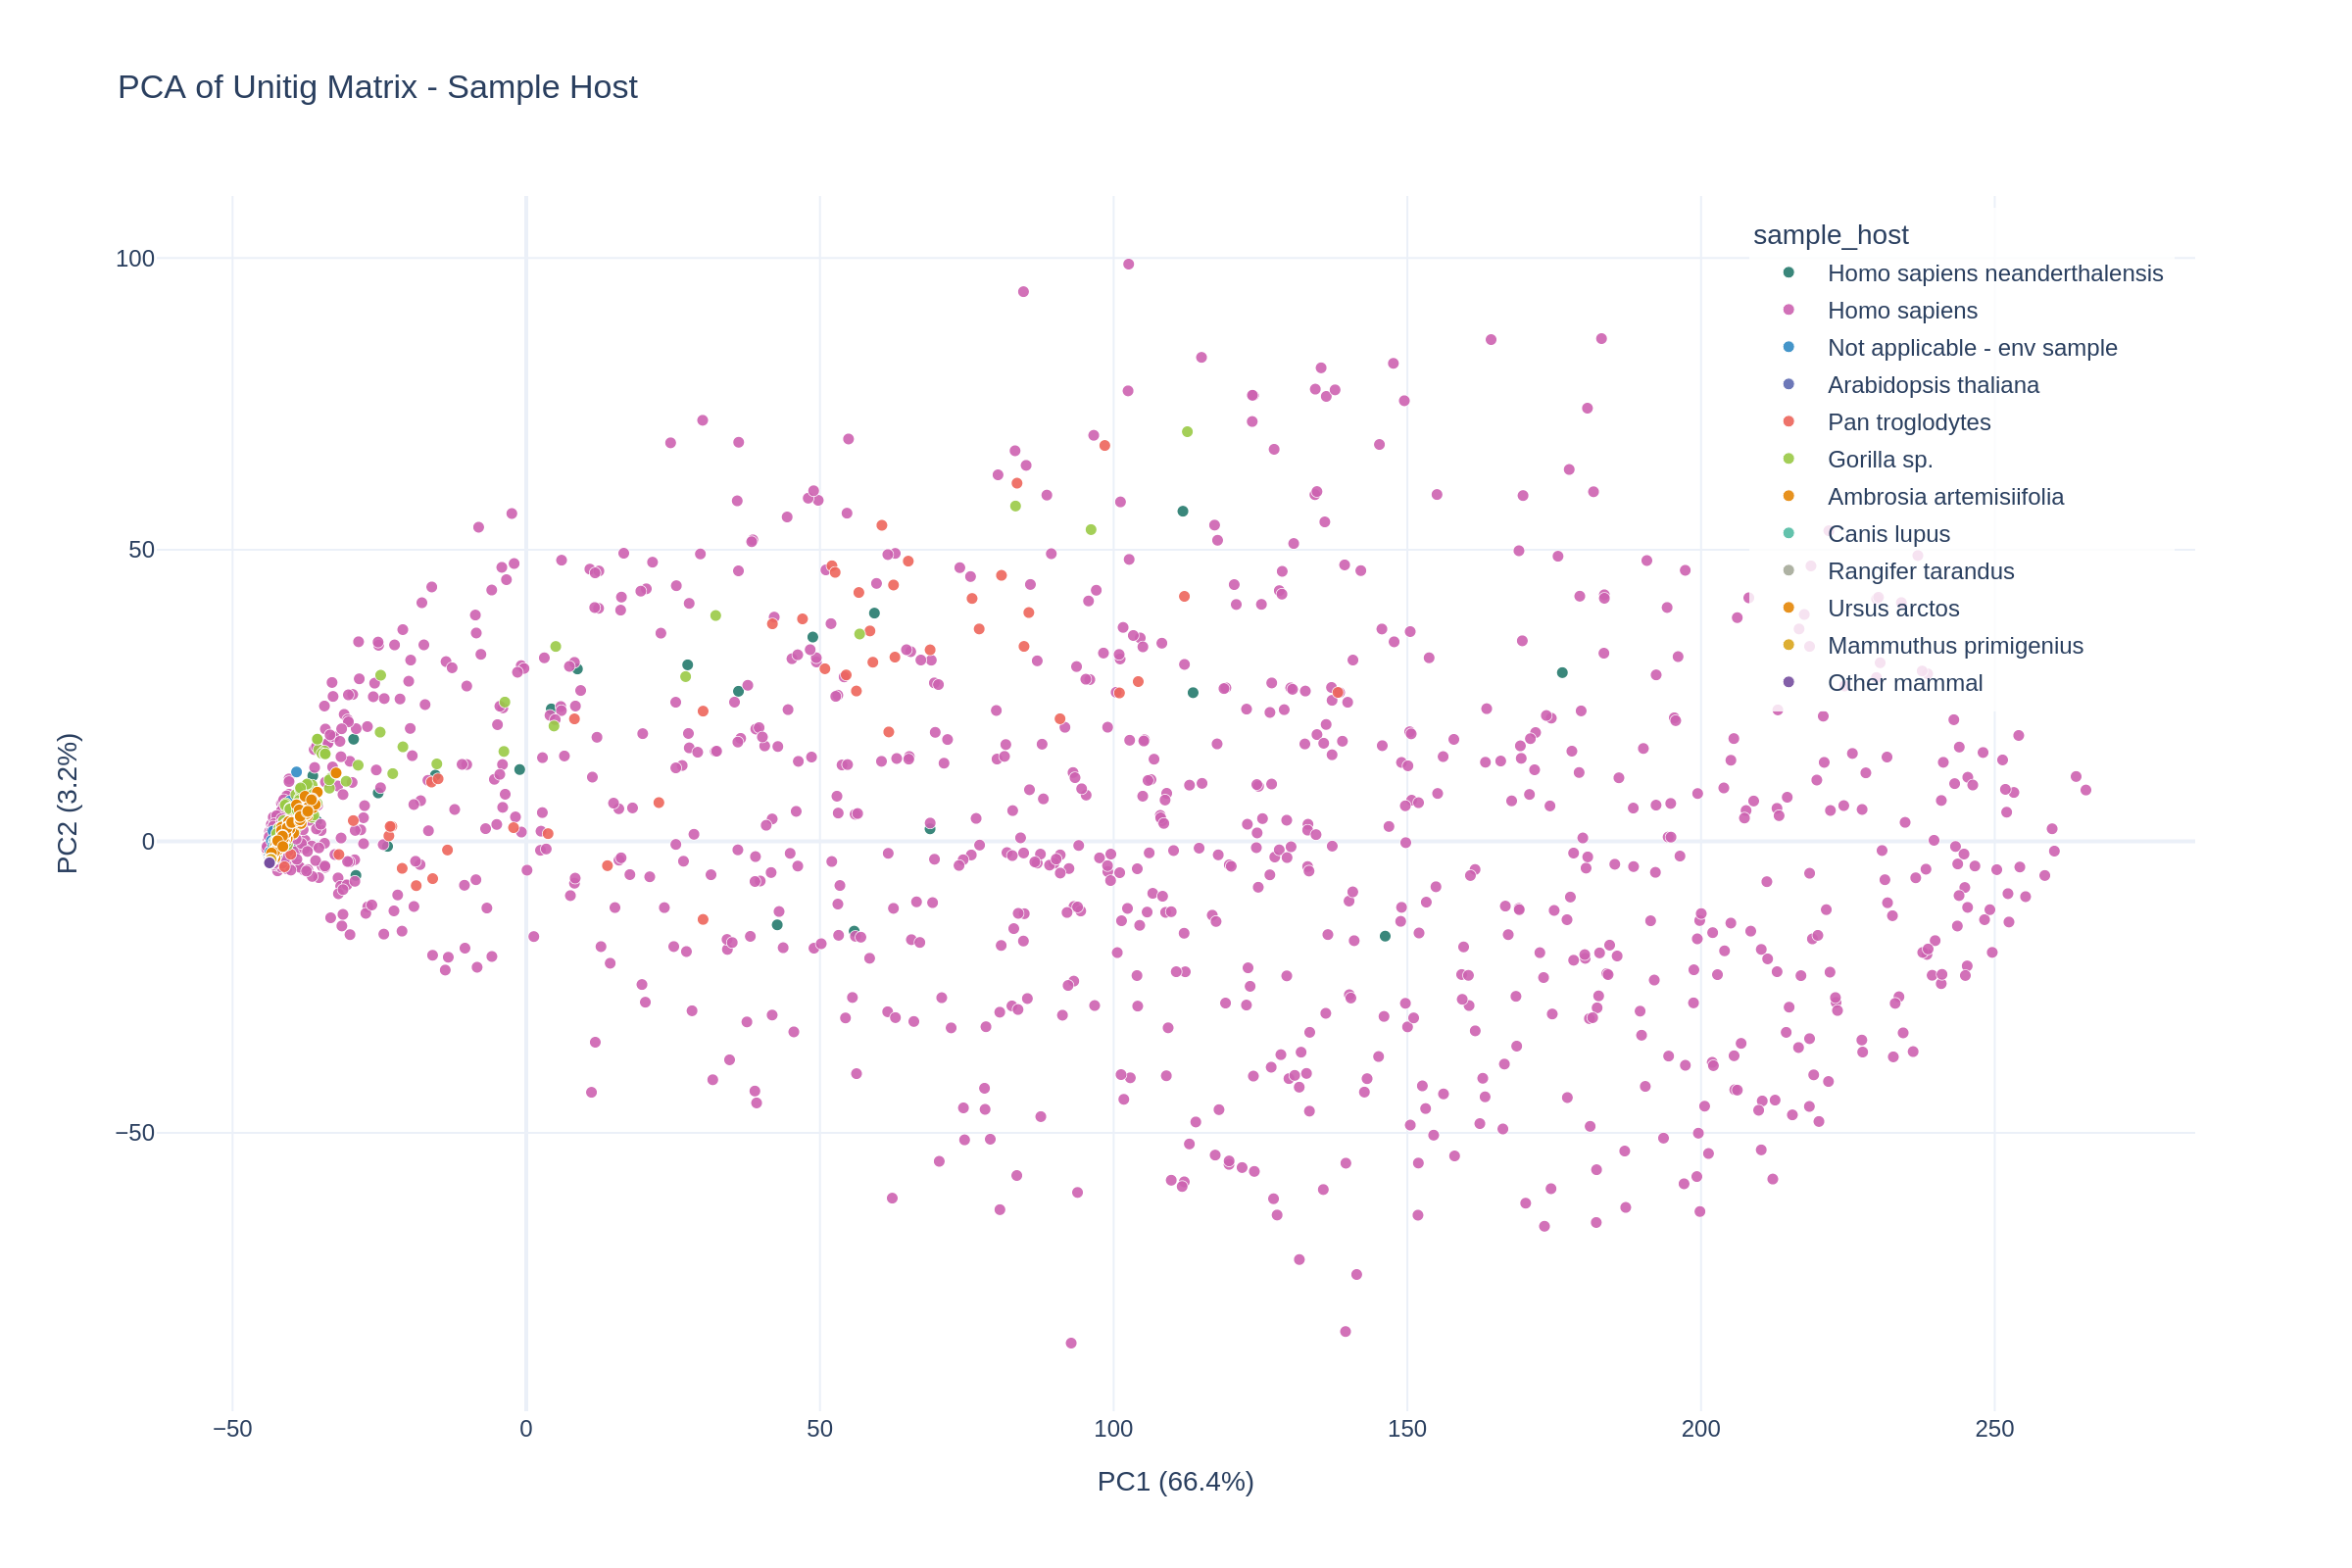
\includegraphics[width=0.48\textwidth]{sup_03_pca_sample_host.png}%
    }
    \hfill
    \subfloat[Material]{%
        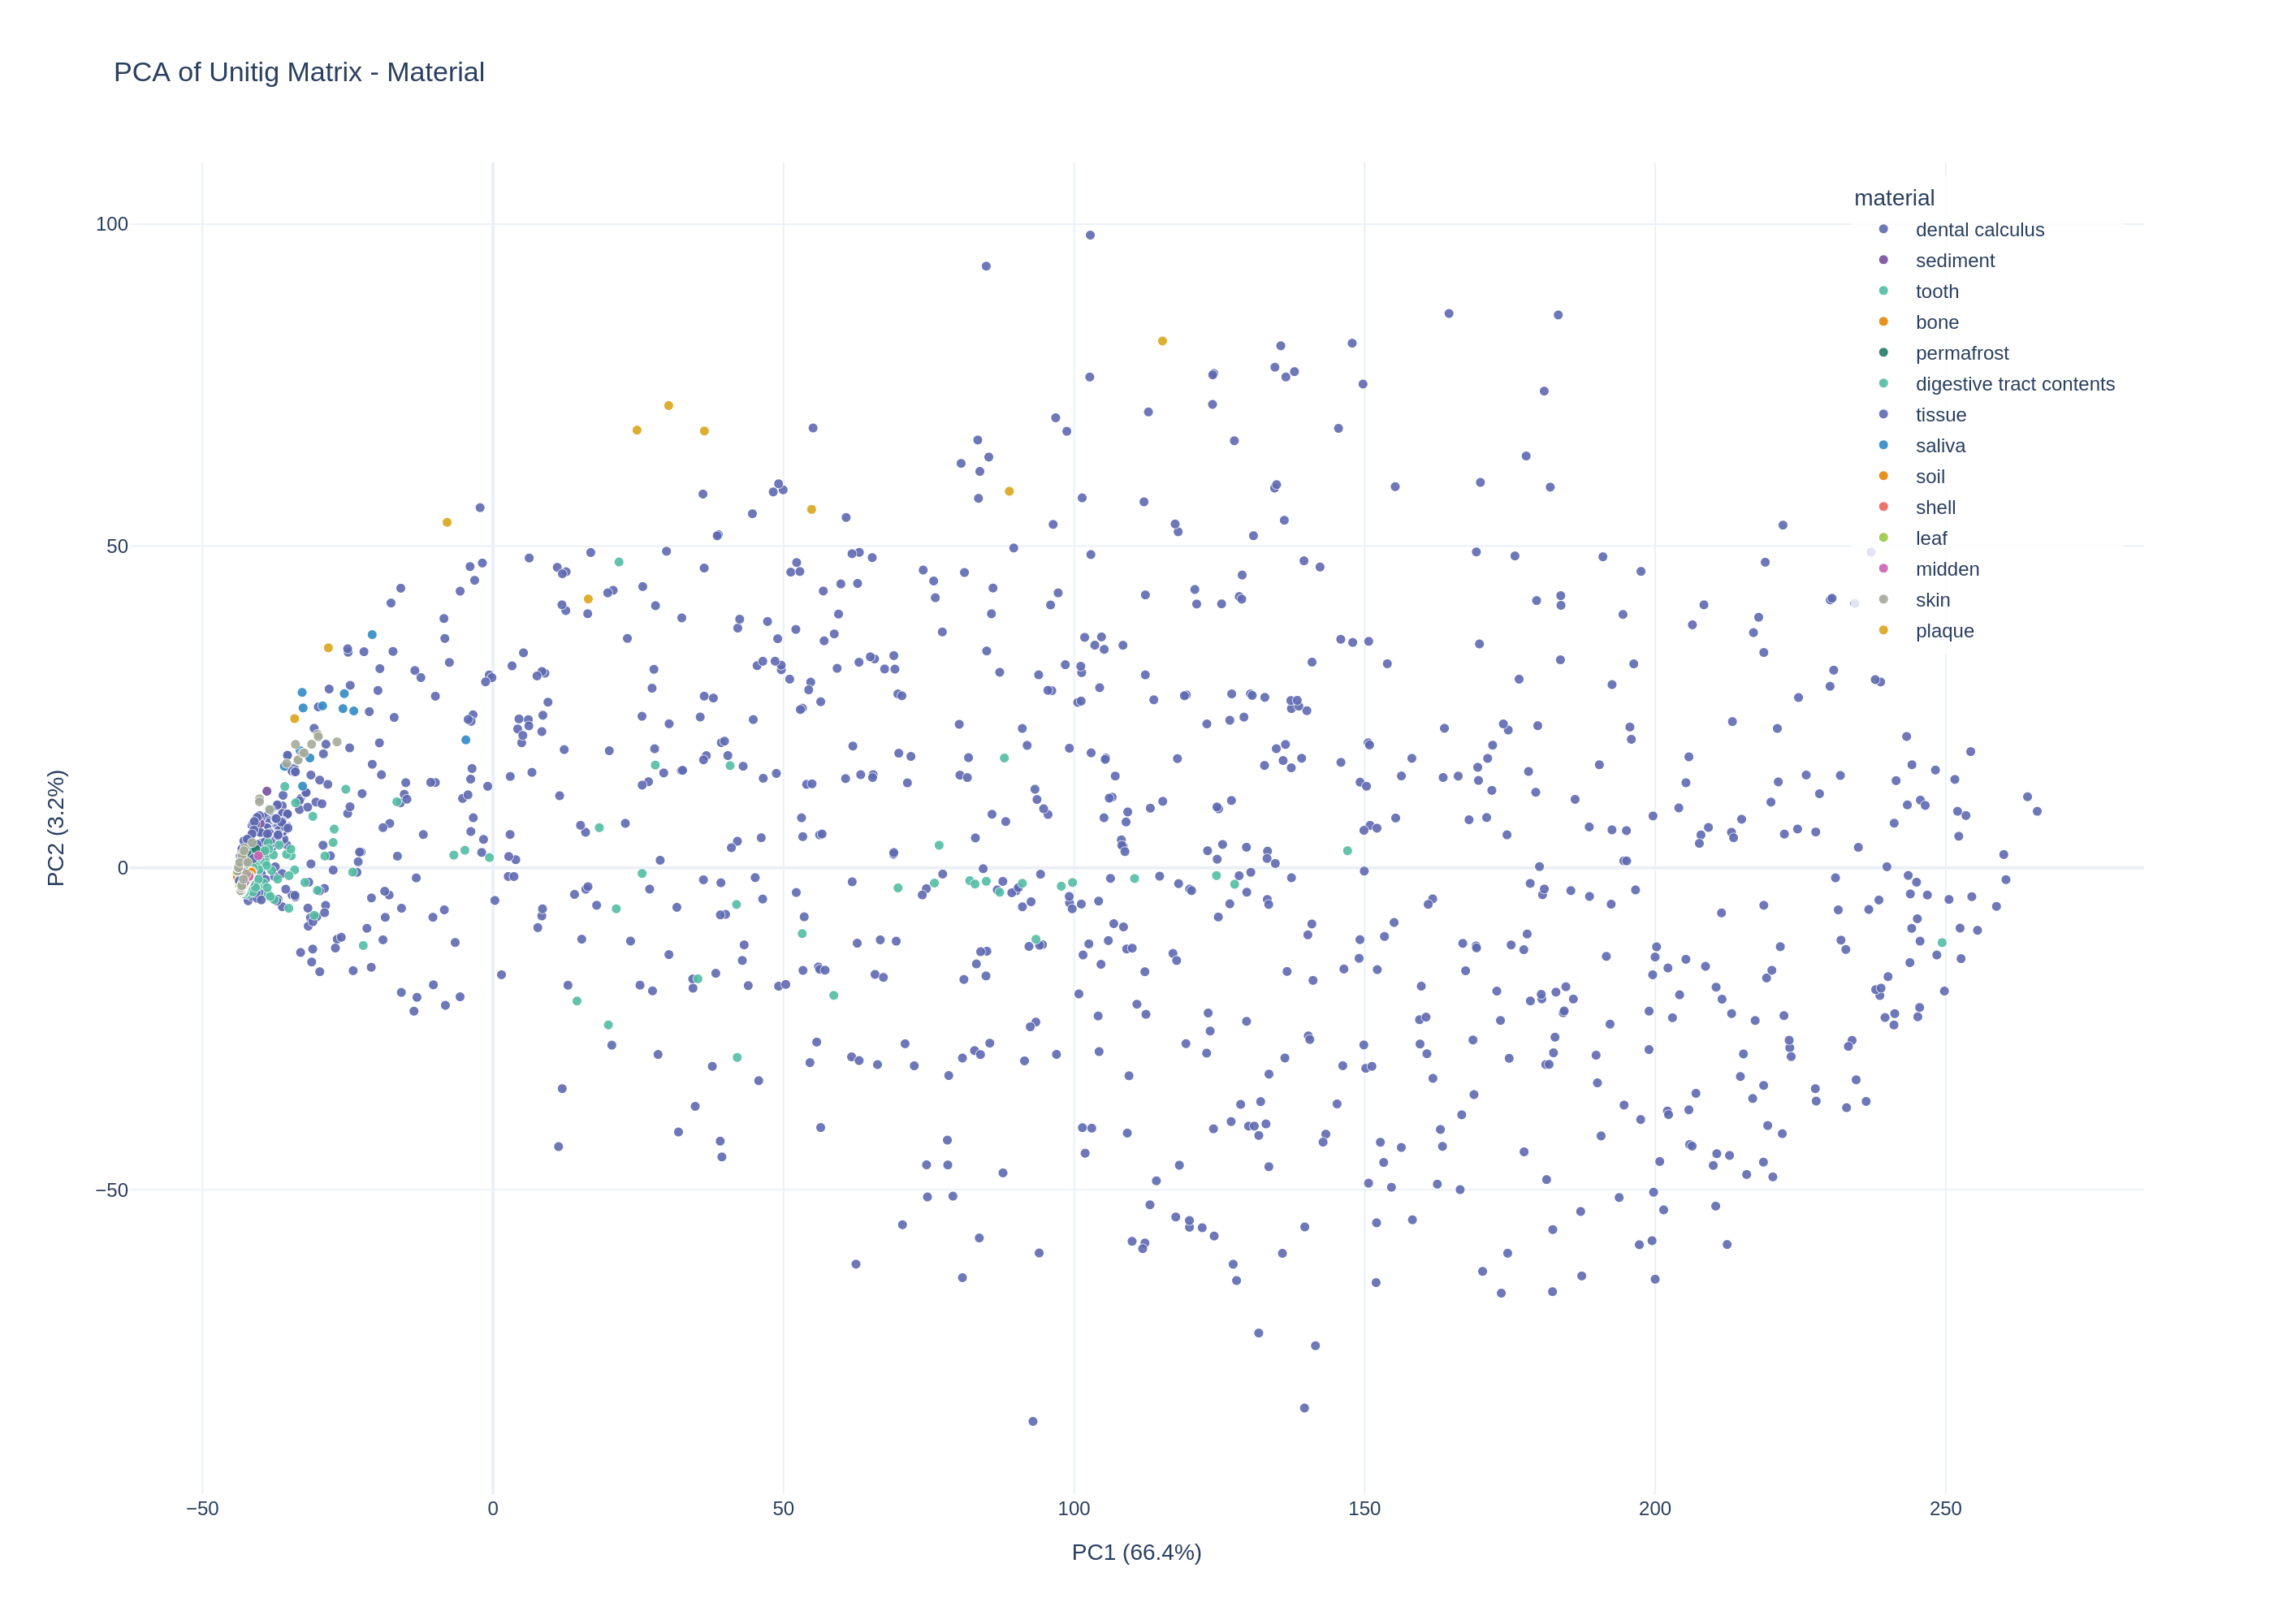
\includegraphics[width=0.48\textwidth]{sup_03_pca_material.png}%
    }
    \caption{\textbf{PCA projections colored by classification task labels.}
    2D projections of training and test samples (n=3,058 total: 2,597 train + 461 test) onto PC1 and PC2, 
    colored by classification task labels.
    (a) Sample type (2 classes: ancient vs. modern) shows partial separation along PC1, 
    with ancient samples more dispersed due to temporal and environmental heterogeneity.
    (b) Community type (6 categories) exhibits overlapping clusters with some tissue-specific separation,
    particularly for oral microbiomes vs. environmental samples.
    (c) Sample host (12 species in training) shows species-specific grouping, 
    with clear separation for environmental samples (Not applicable - env sample) from host-associated samples.
    (d) Material (13 types in training) demonstrates substrate-specific patterns, 
    with dental calculus, bone, and sediment forming distinct clusters.
    PCA computed on 107,480 unitig features. 
    Limited separation in PC1-PC2 space demonstrates the challenge of linearly separable classification,
    motivating the use of deep neural networks for multitask learning.
    }
    \addcontentsline{toc}{subsection}{\protect\numberline{\thefigure}PCA projections by task}
    \label{fig:sup_pca_projections}
\end{figure}

\clearpage

% ===================================================================
% Supplementary Figure N: PCA Projections by Task (PC3 vs PC4)
% ===================================================================
\begin{figure}[p]
    \centering
    \subfloat[Sample Type]{%
        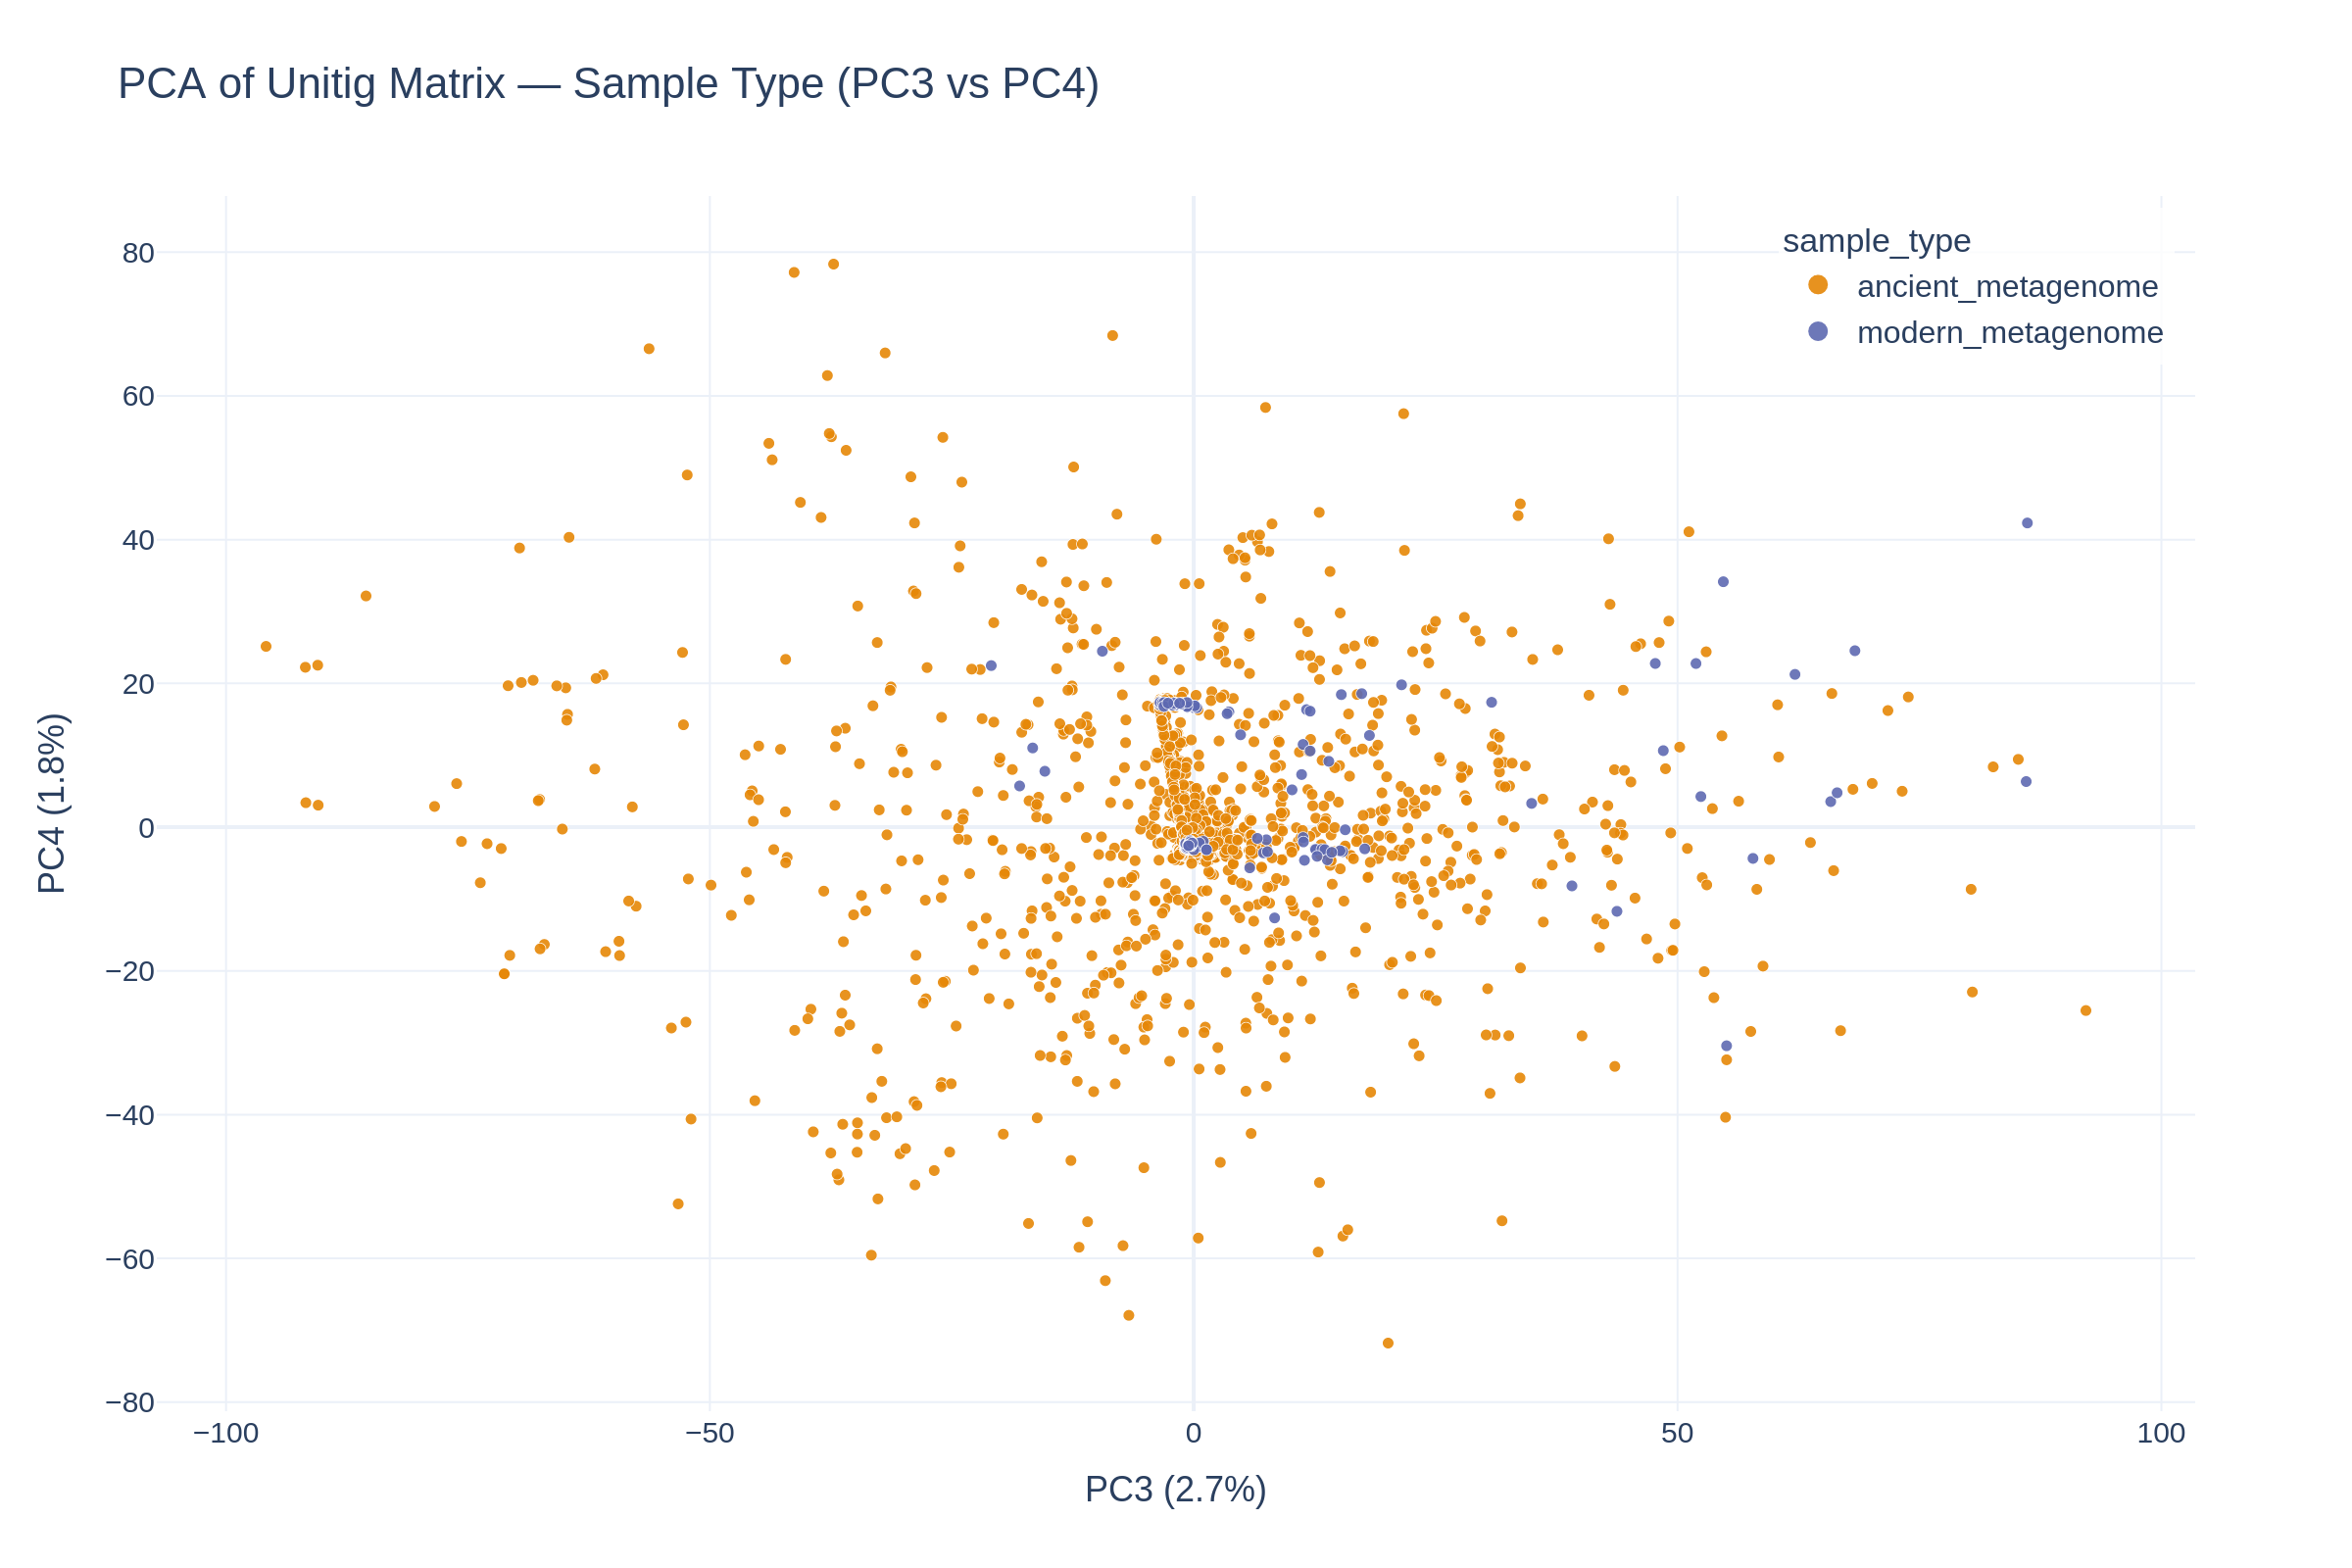
\includegraphics[width=0.48\textwidth]{sup_03_pca_sample_type_pc34.png}%
    }
    \hfill
    \subfloat[Community Type]{%
        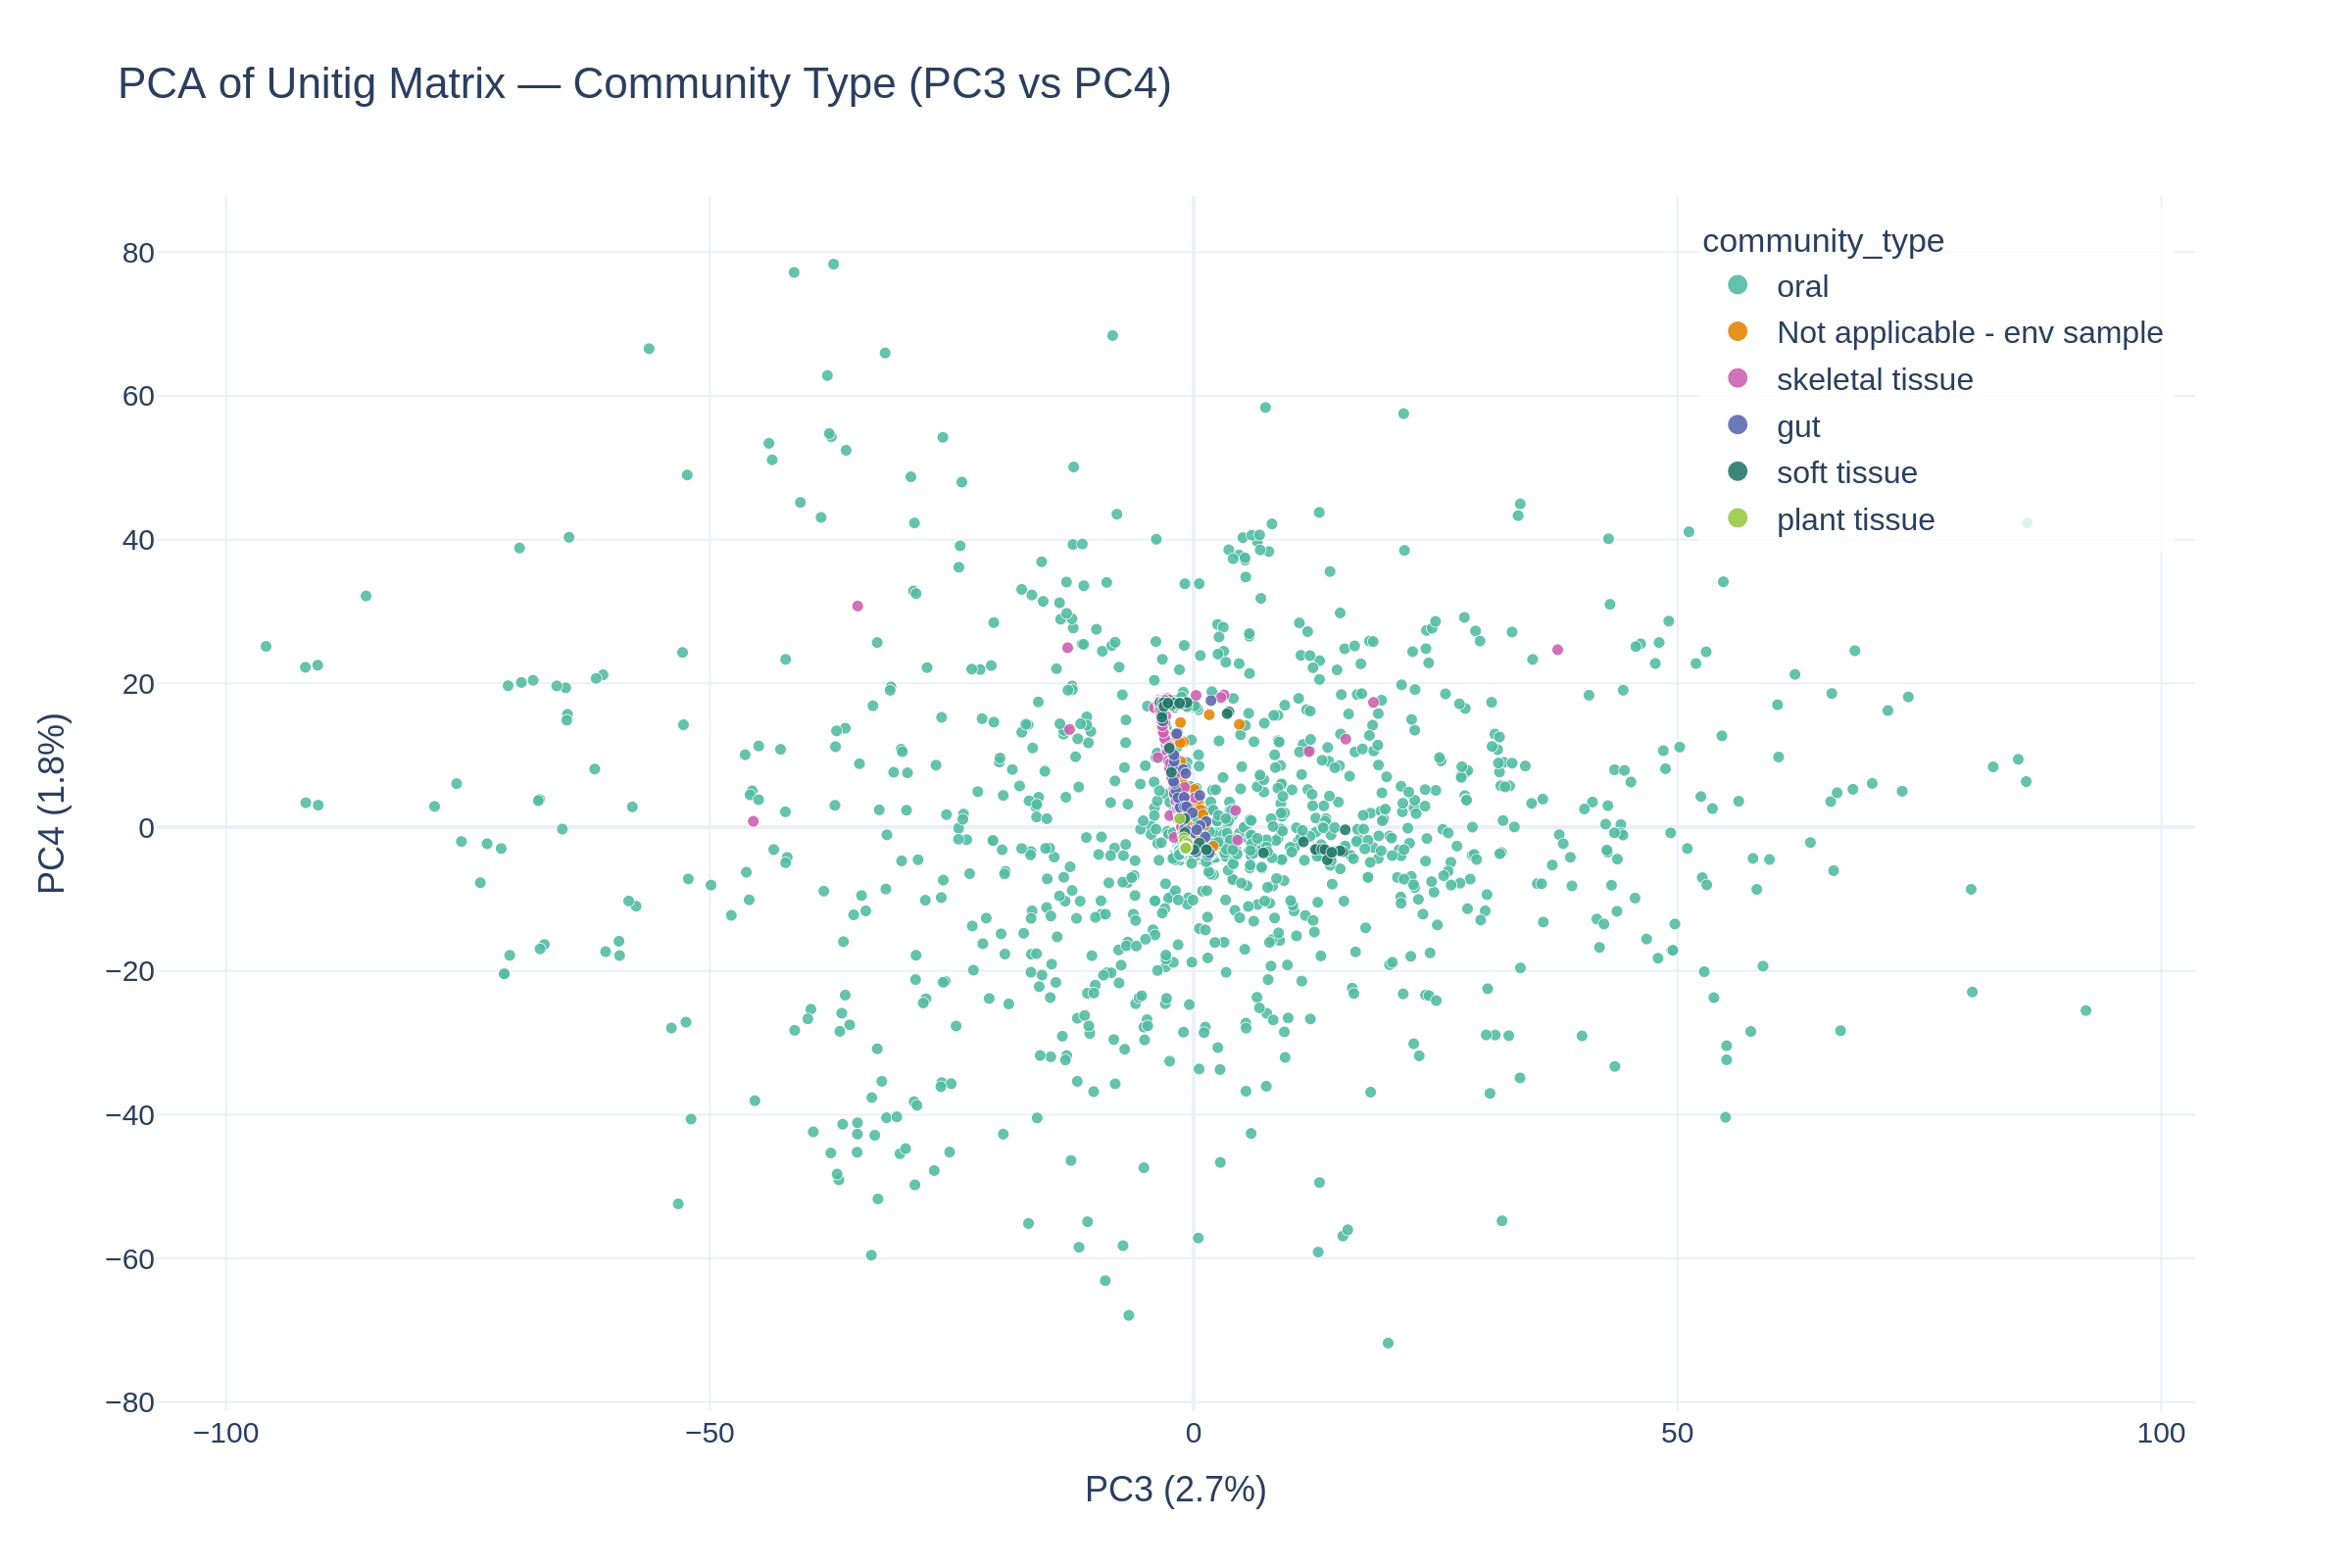
\includegraphics[width=0.48\textwidth]{sup_03_pca_community_type_pc34.png}%
    }
    \\
    \subfloat[Sample Host]{%
        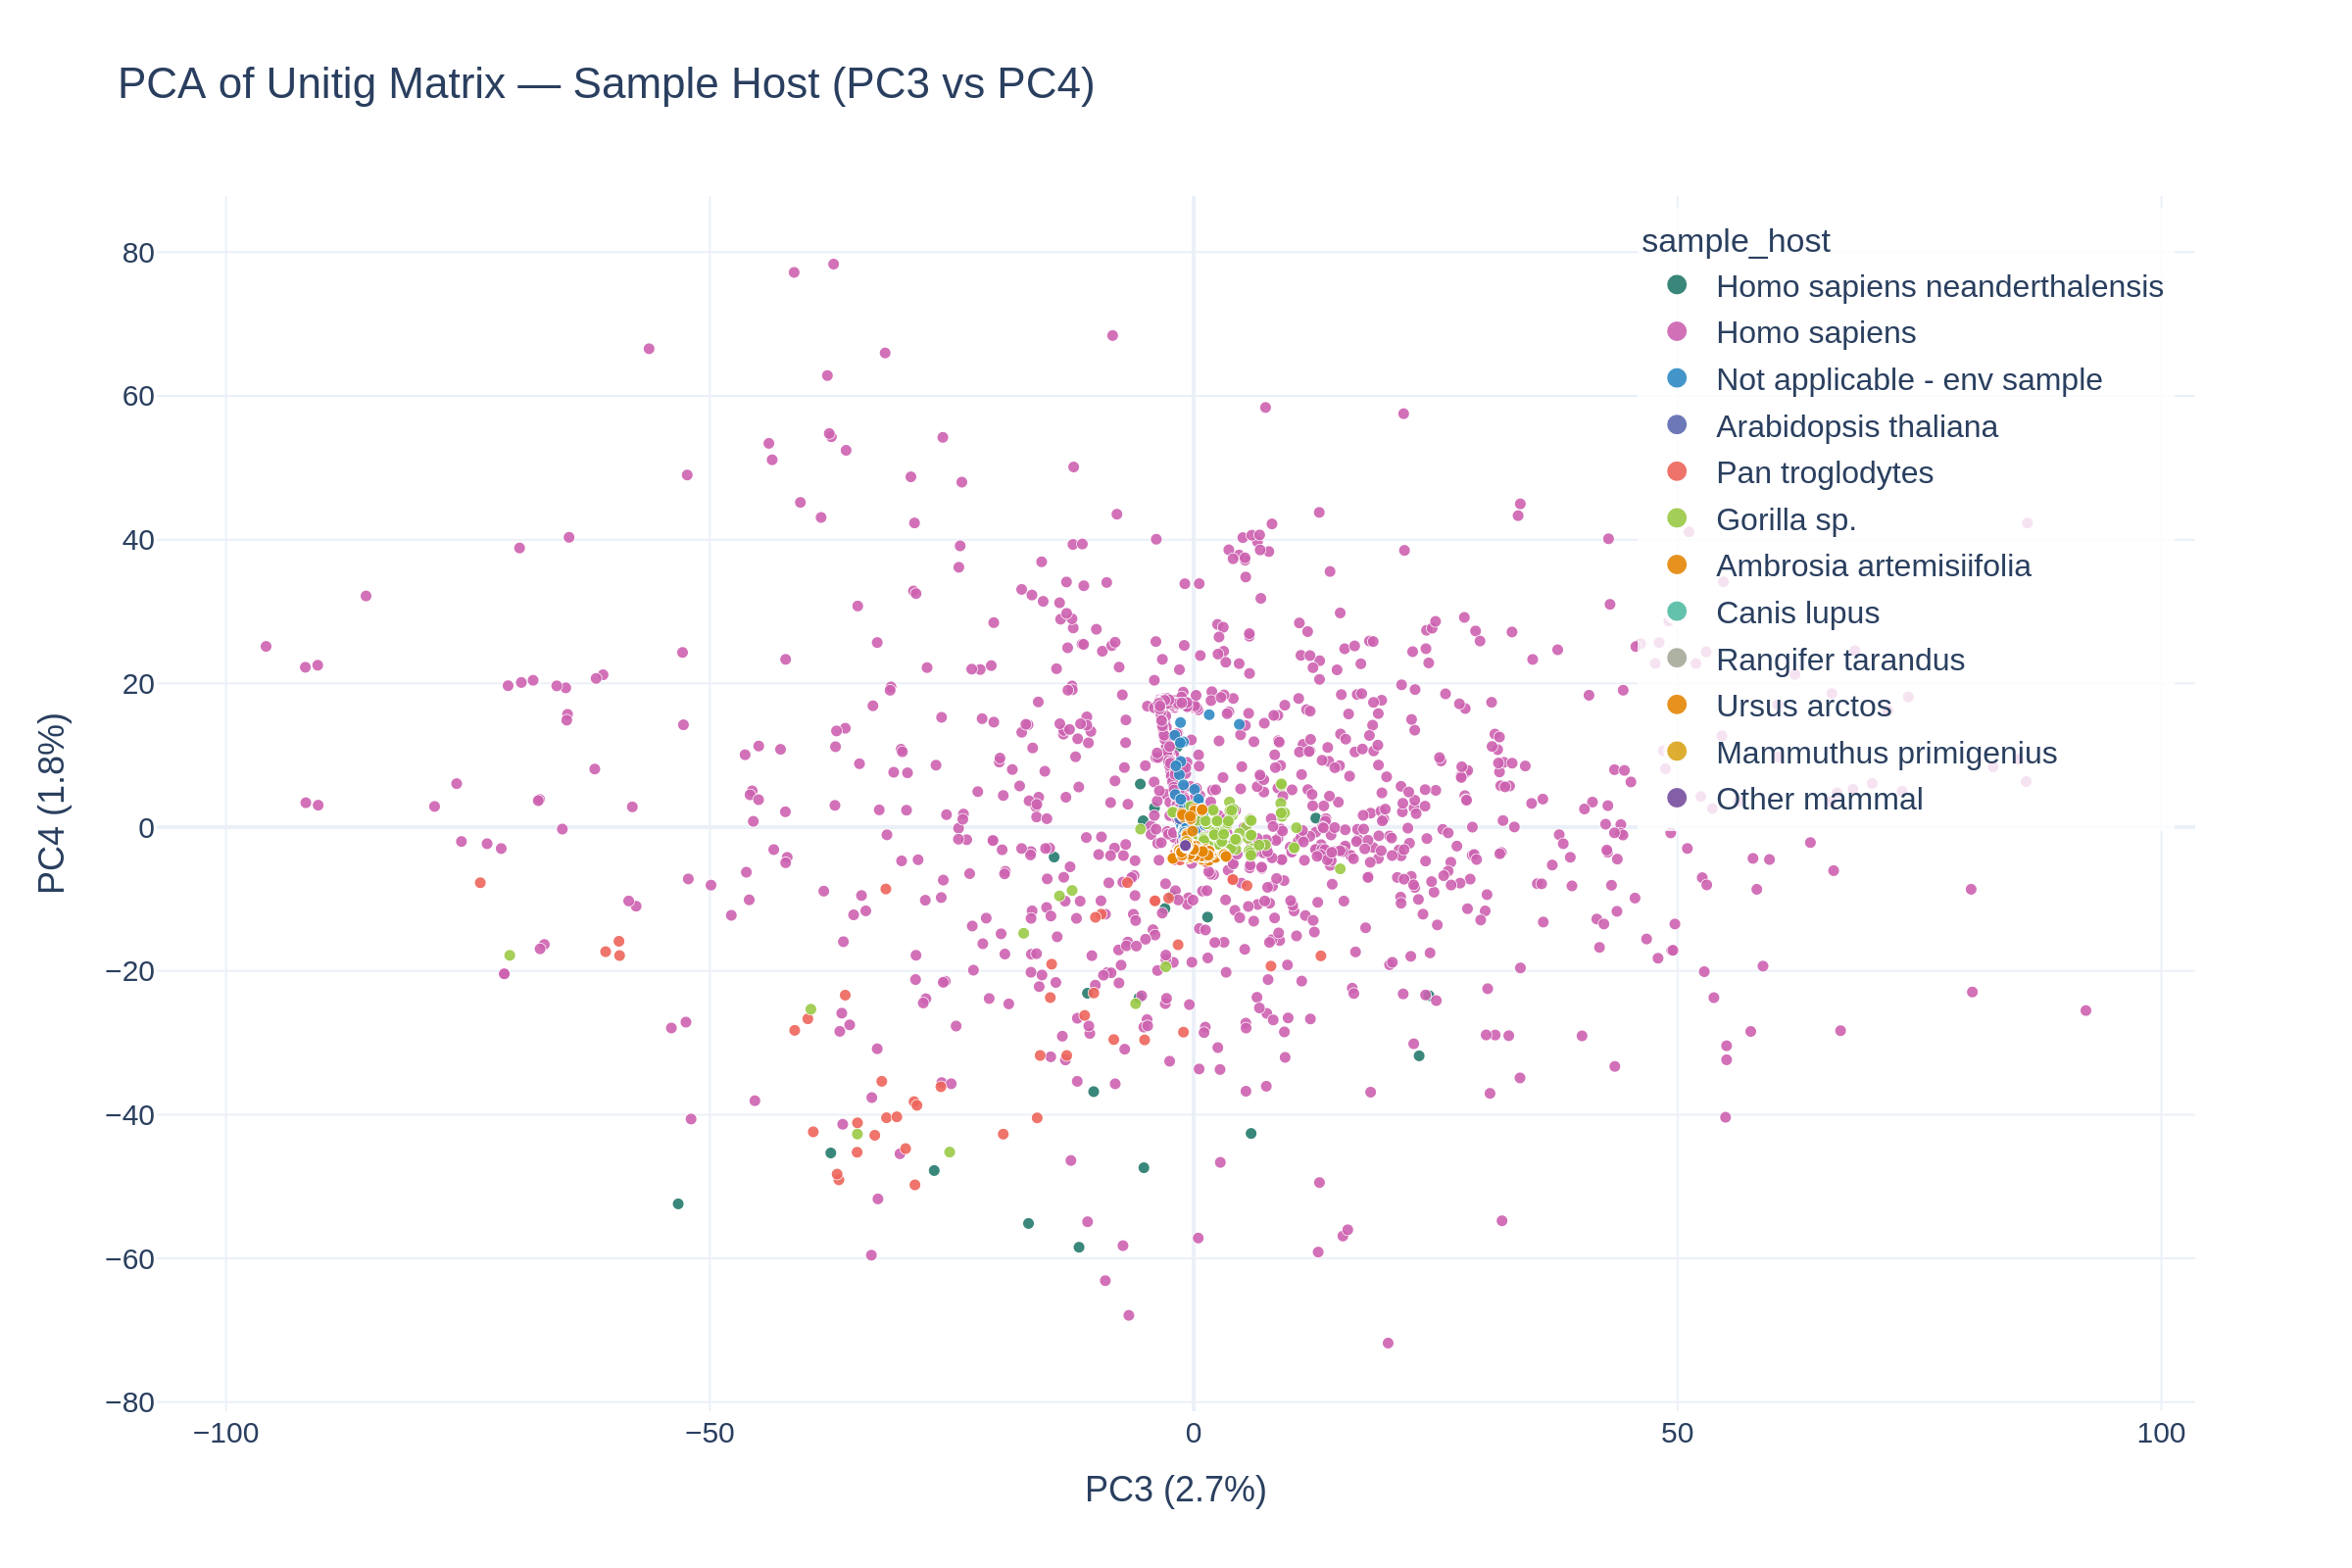
\includegraphics[width=0.48\textwidth]{sup_03_pca_sample_host_pc34.png}%
    }
    \hfill
    \subfloat[Material]{%
        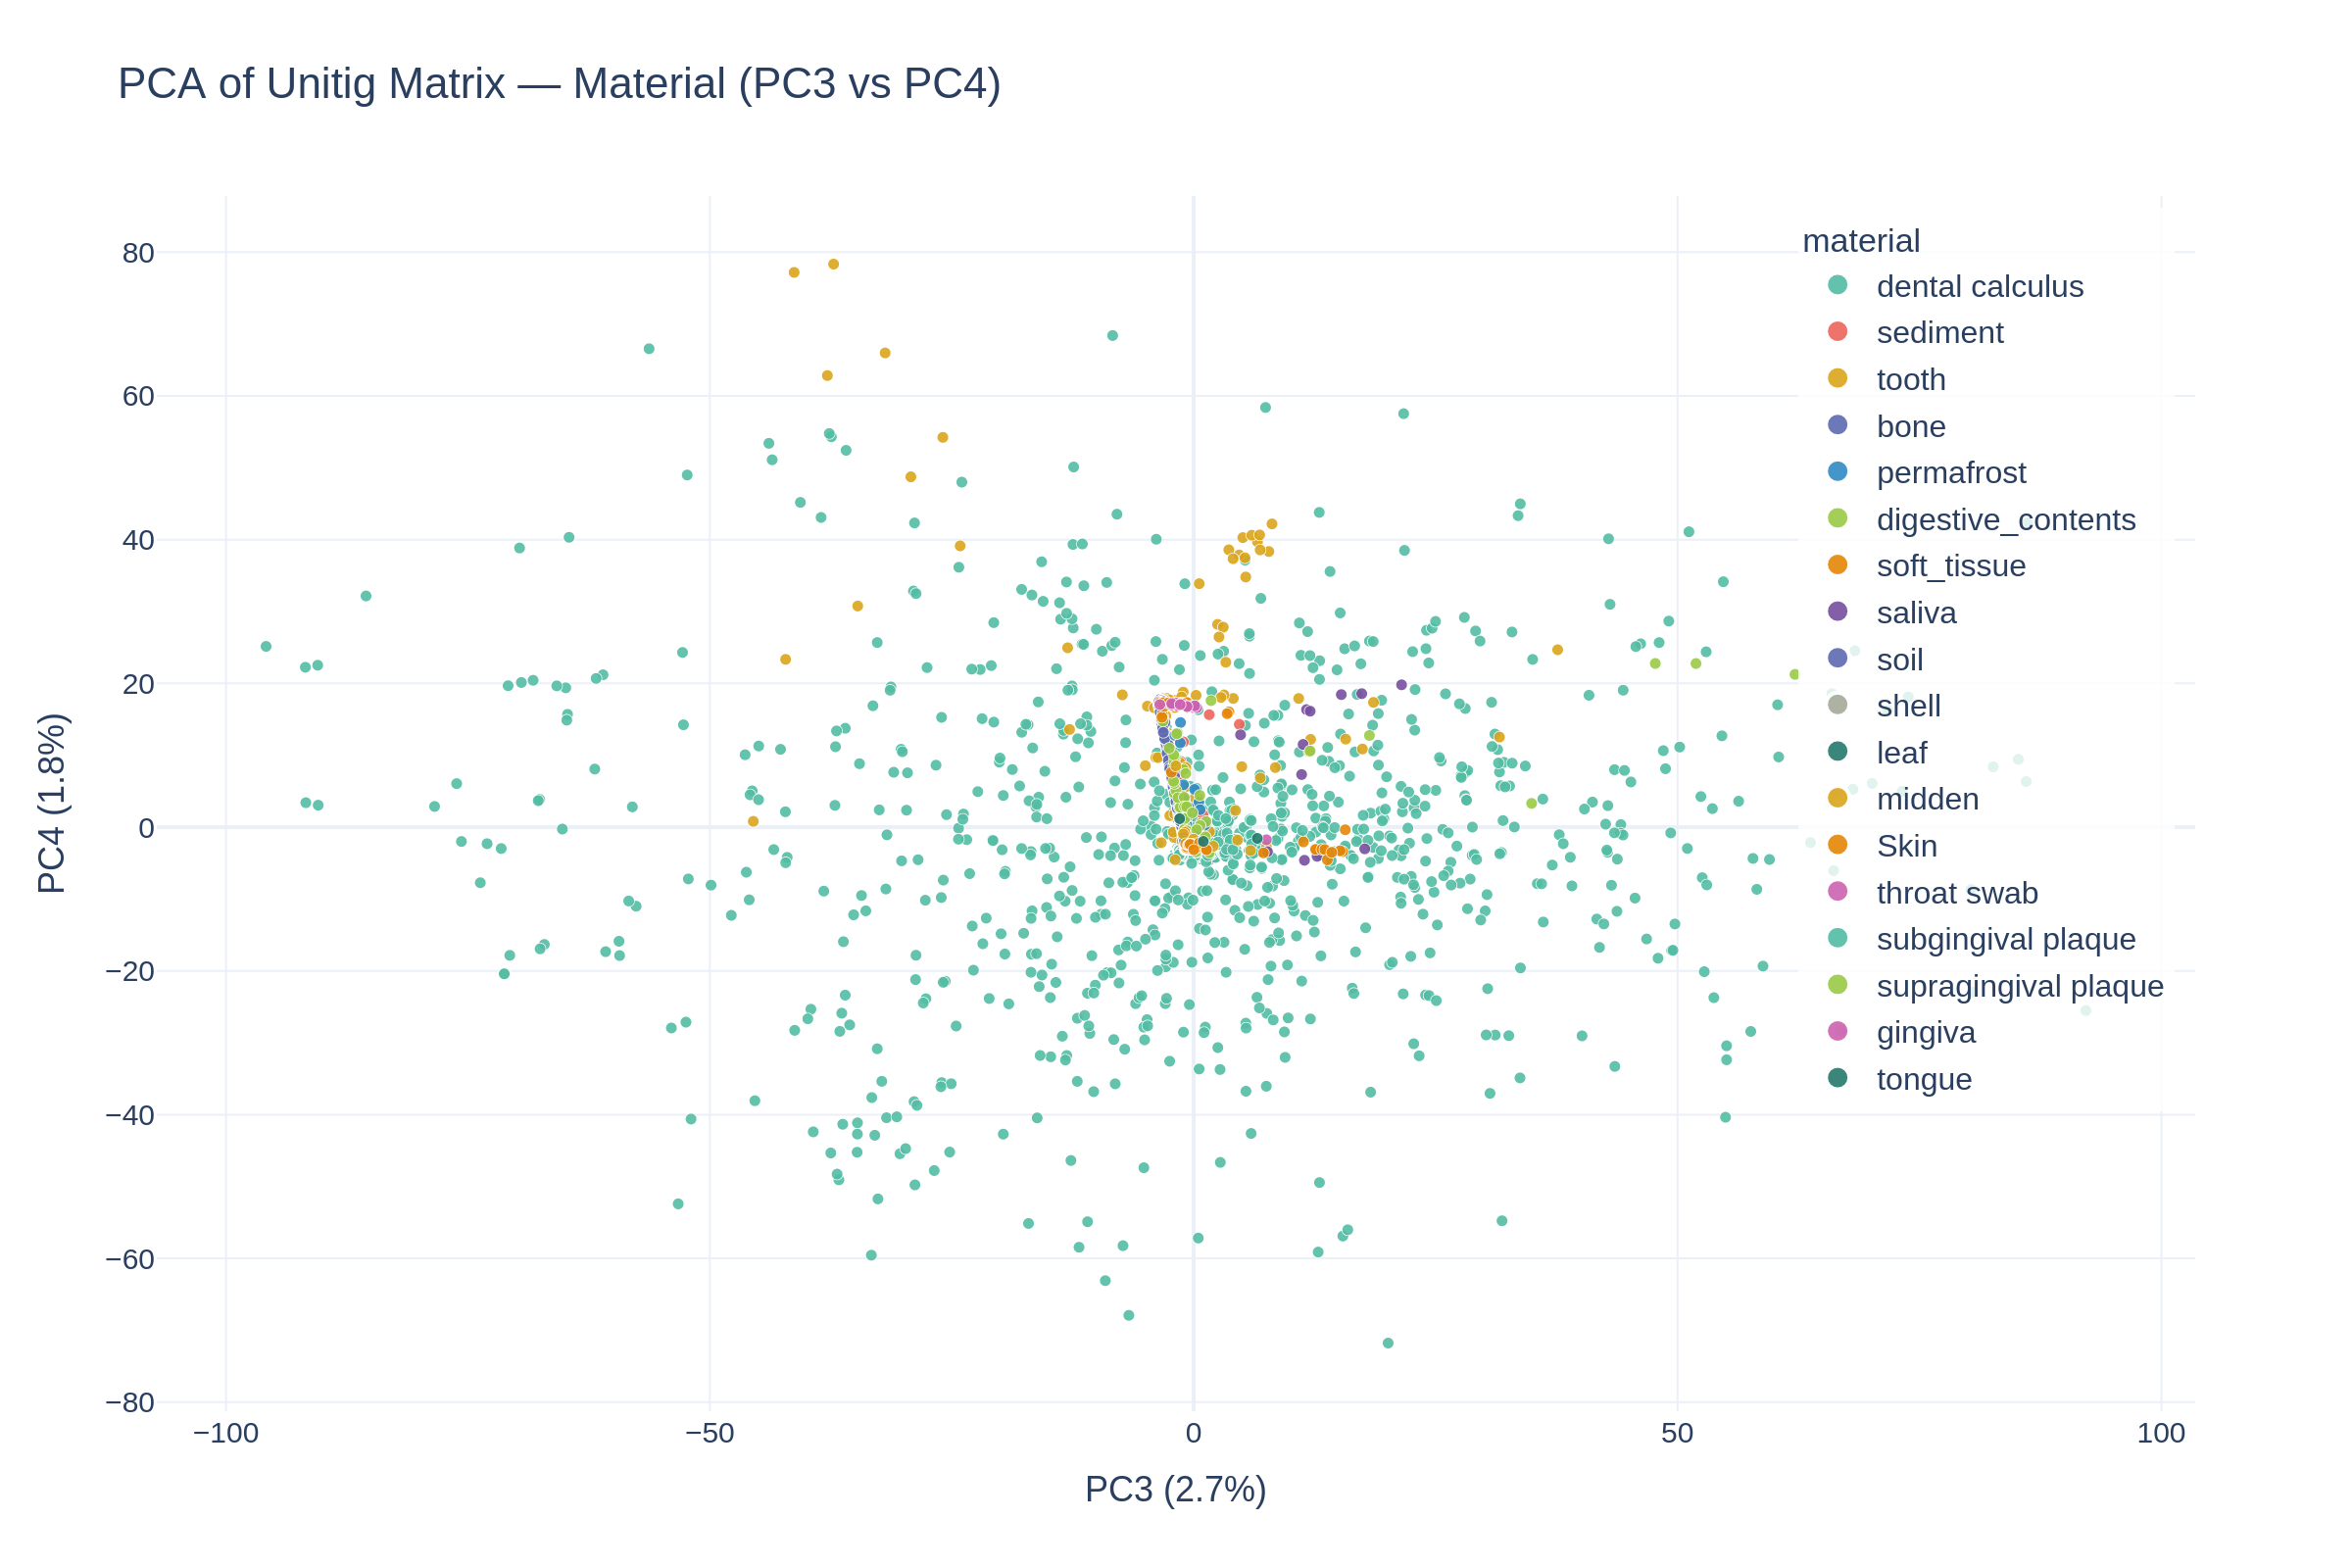
\includegraphics[width=0.48\textwidth]{sup_03_pca_material_pc34.png}%
    }
    \caption{\textbf{PCA projections along PC3 and PC4 colored by classification task labels.}
    2D projections of training and test samples (n=3,058 total: 2,597 train + 461 test) onto
    PC3 and PC4, colored by classification task labels.
    Compare with the PC1--PC2 projections (previous figure) to assess whether higher principal
    components reveal additional class structure or separation not apparent in the first two.
    PC3 and PC4 each explain less individual variance than PC1 and PC2, but may capture
    task-specific signal orthogonal to the dominant axes of variation.
    PCA computed on 107,480 unitig features.
    }
    \addcontentsline{toc}{subsection}{\protect\numberline{\thefigure}PCA PC3 vs PC4 projections by task}
    \label{fig:sup_pca_projections_pc34}
\end{figure}

% ===================================================================
% Supplementary Figure: Unitig PCA Loadings by Species
% ===================================================================
\begin{figure}[p]
    \centering
    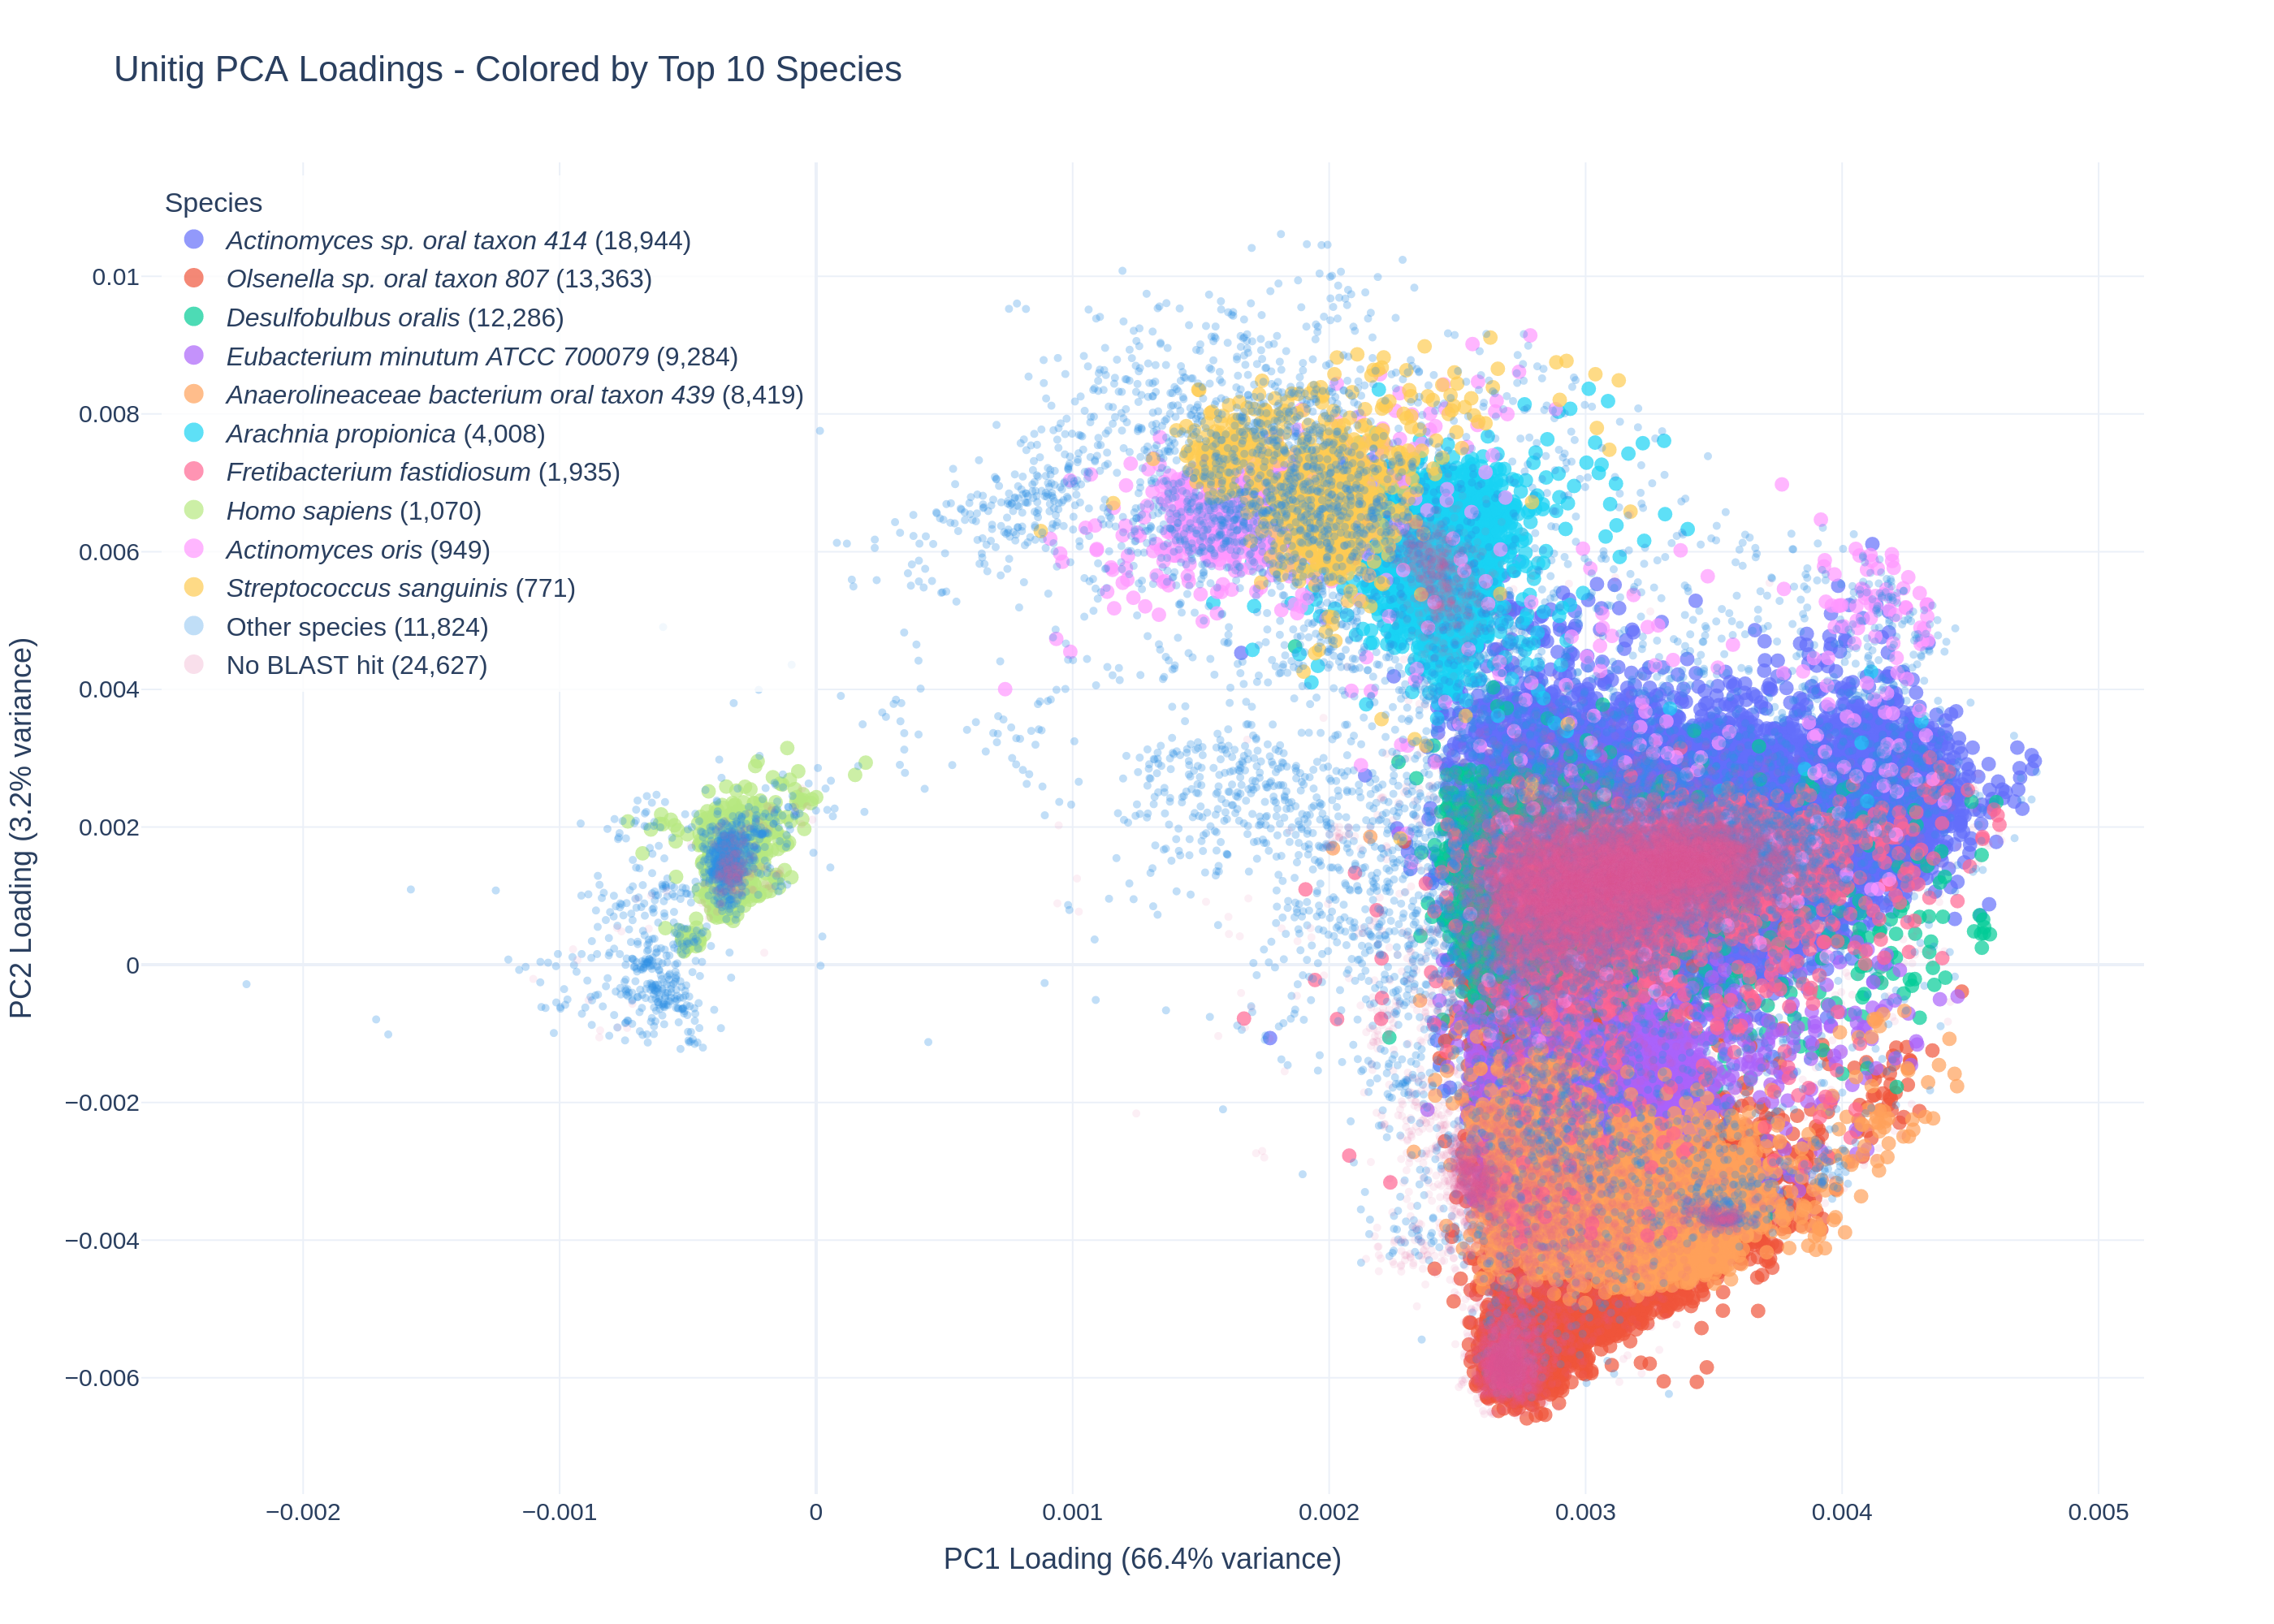
\includegraphics[width=0.95\textwidth]{sup_04_pca_unitig_loadings_by_species.png}
    \caption{\textbf{Unitig PCA loadings colored by taxonomic species.}
    Scatter plot showing PC1 and PC2 loadings for all 107,480 unitig features, 
    colored by the top 20 most abundant species from BLAST annotations. 
    Points represent individual unitigs, with position indicating their contribution to each principal component. 
    Species with largest numbers of annotated unitigs are shown in distinct colors, 
    while other species and unannotated unitigs are displayed in light gray for context. 
    This visualization reveals the taxonomic distribution of discriminative features driving sample separation in PCA space.
    }
    \addcontentsline{toc}{subsection}{\protect\numberline{\thefigure}Unitig loadings by species}
    \label{fig:sup_unitig_loadings}
\end{figure}

% ===================================================================
% Supplementary Figure 7: Feature Importance by Task
% ===================================================================
\begin{figure}[p]
    \centering
    \subfloat[Sample Type]{%
        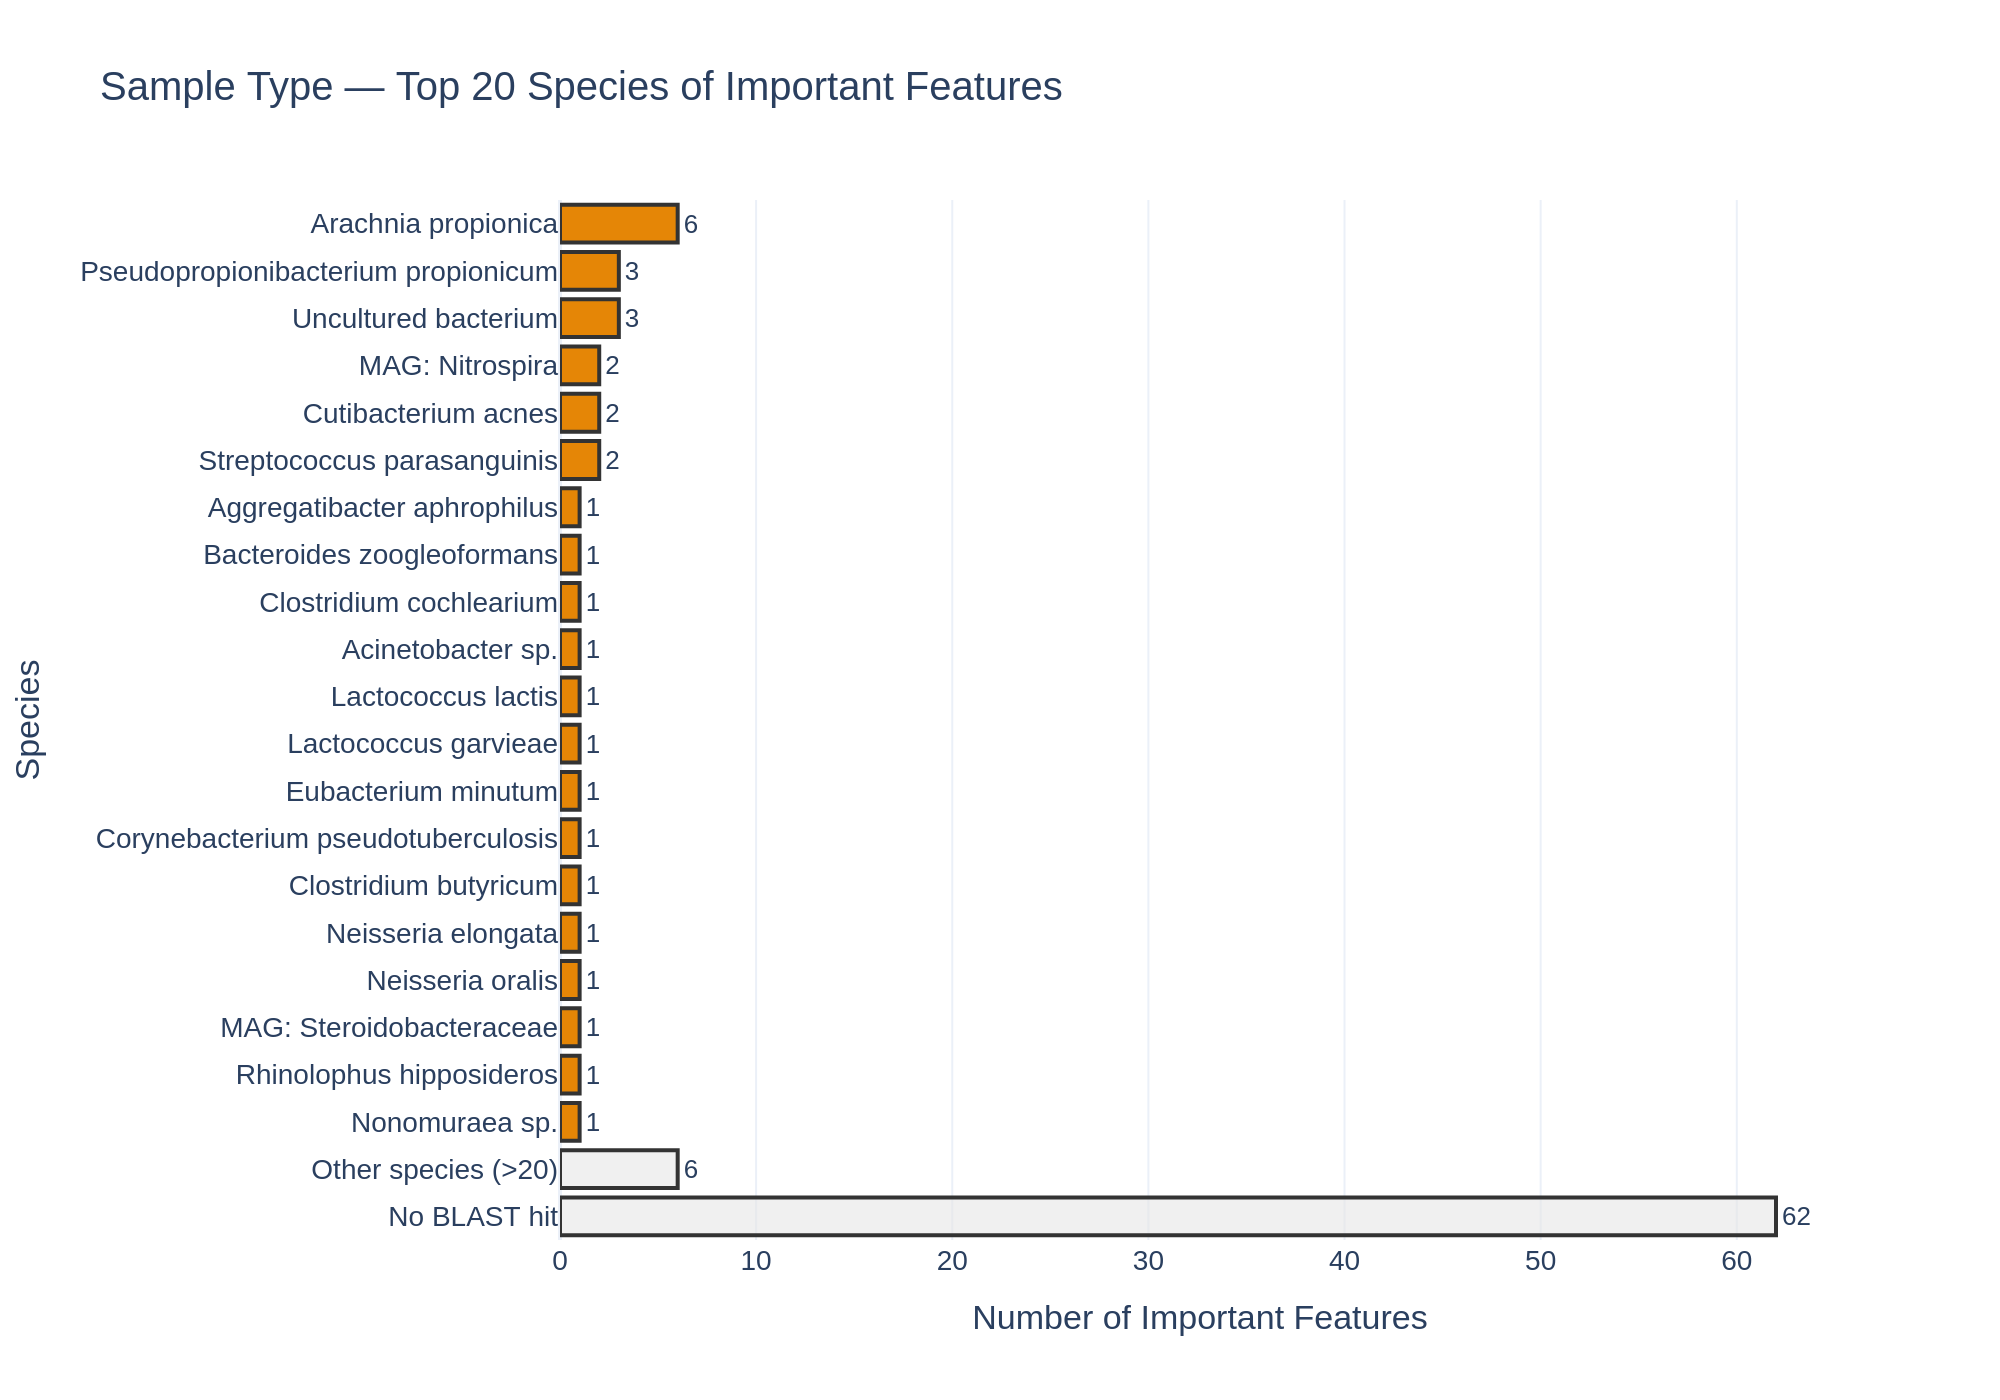
\includegraphics[width=0.49\textwidth]{main_03_feature_importance_sample_type.png}%
    }
    \hfill
    \subfloat[Community Type]{%
        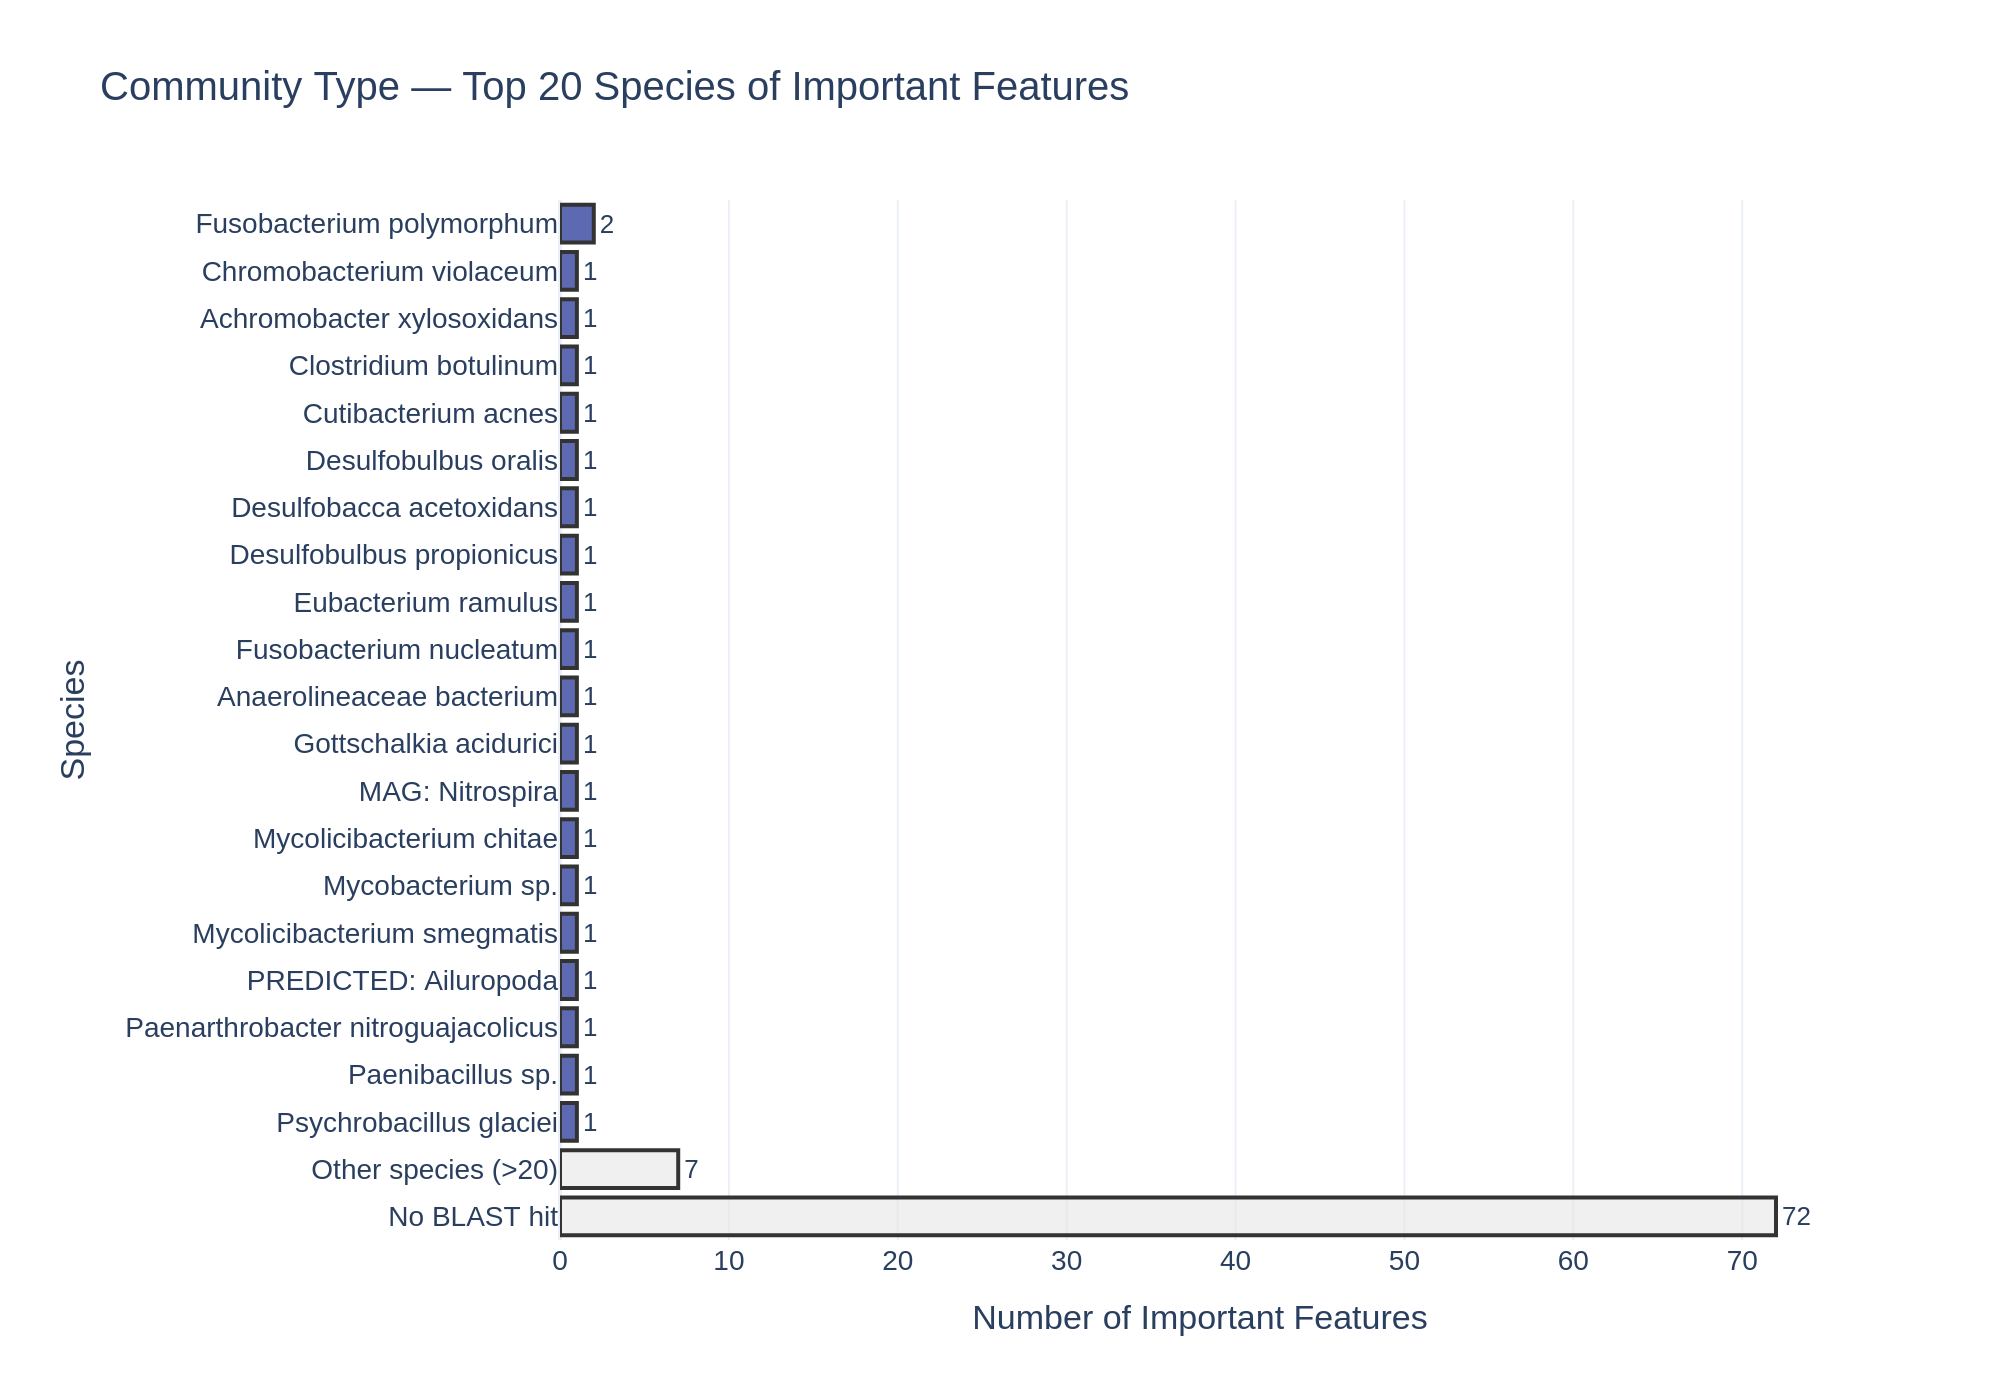
\includegraphics[width=0.49\textwidth]{main_03_feature_importance_community_type.png}%
    }
    \\
    \subfloat[Sample Host]{%
        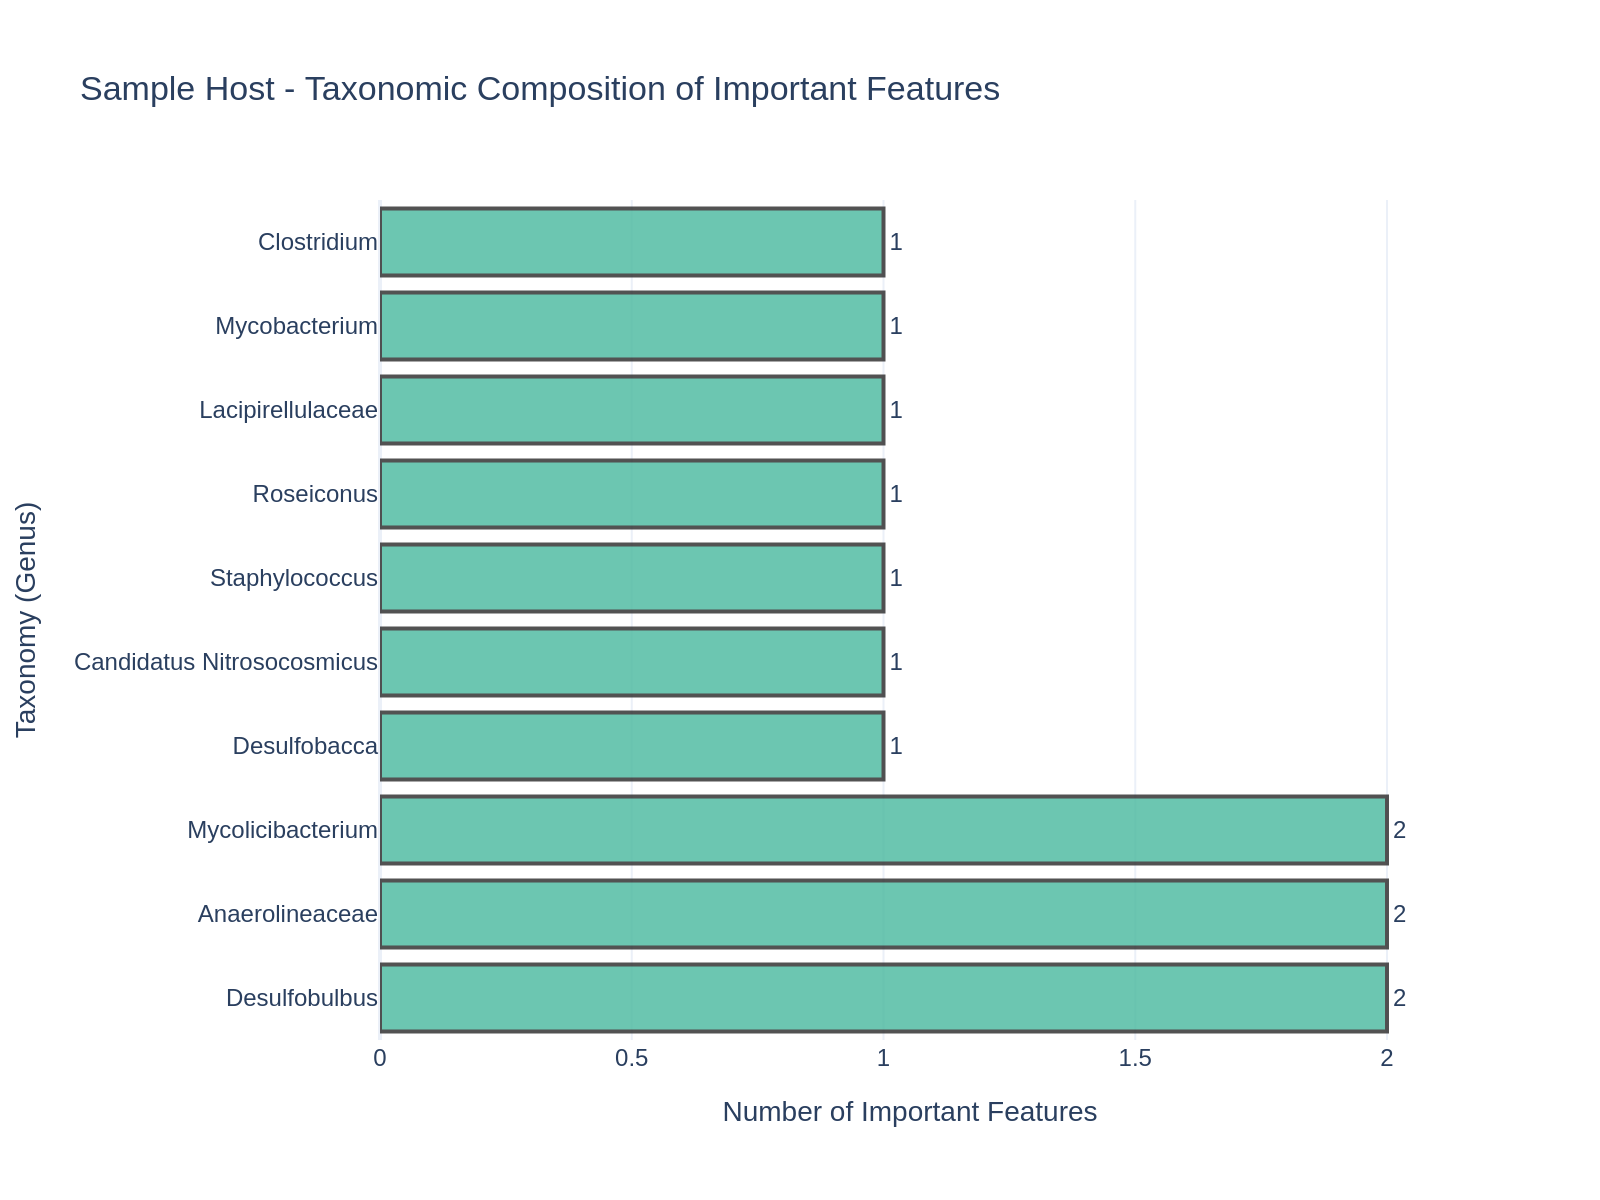
\includegraphics[width=0.49\textwidth]{main_03_feature_importance_sample_host.png}%
    }
    \hfill
    \subfloat[Material]{%
        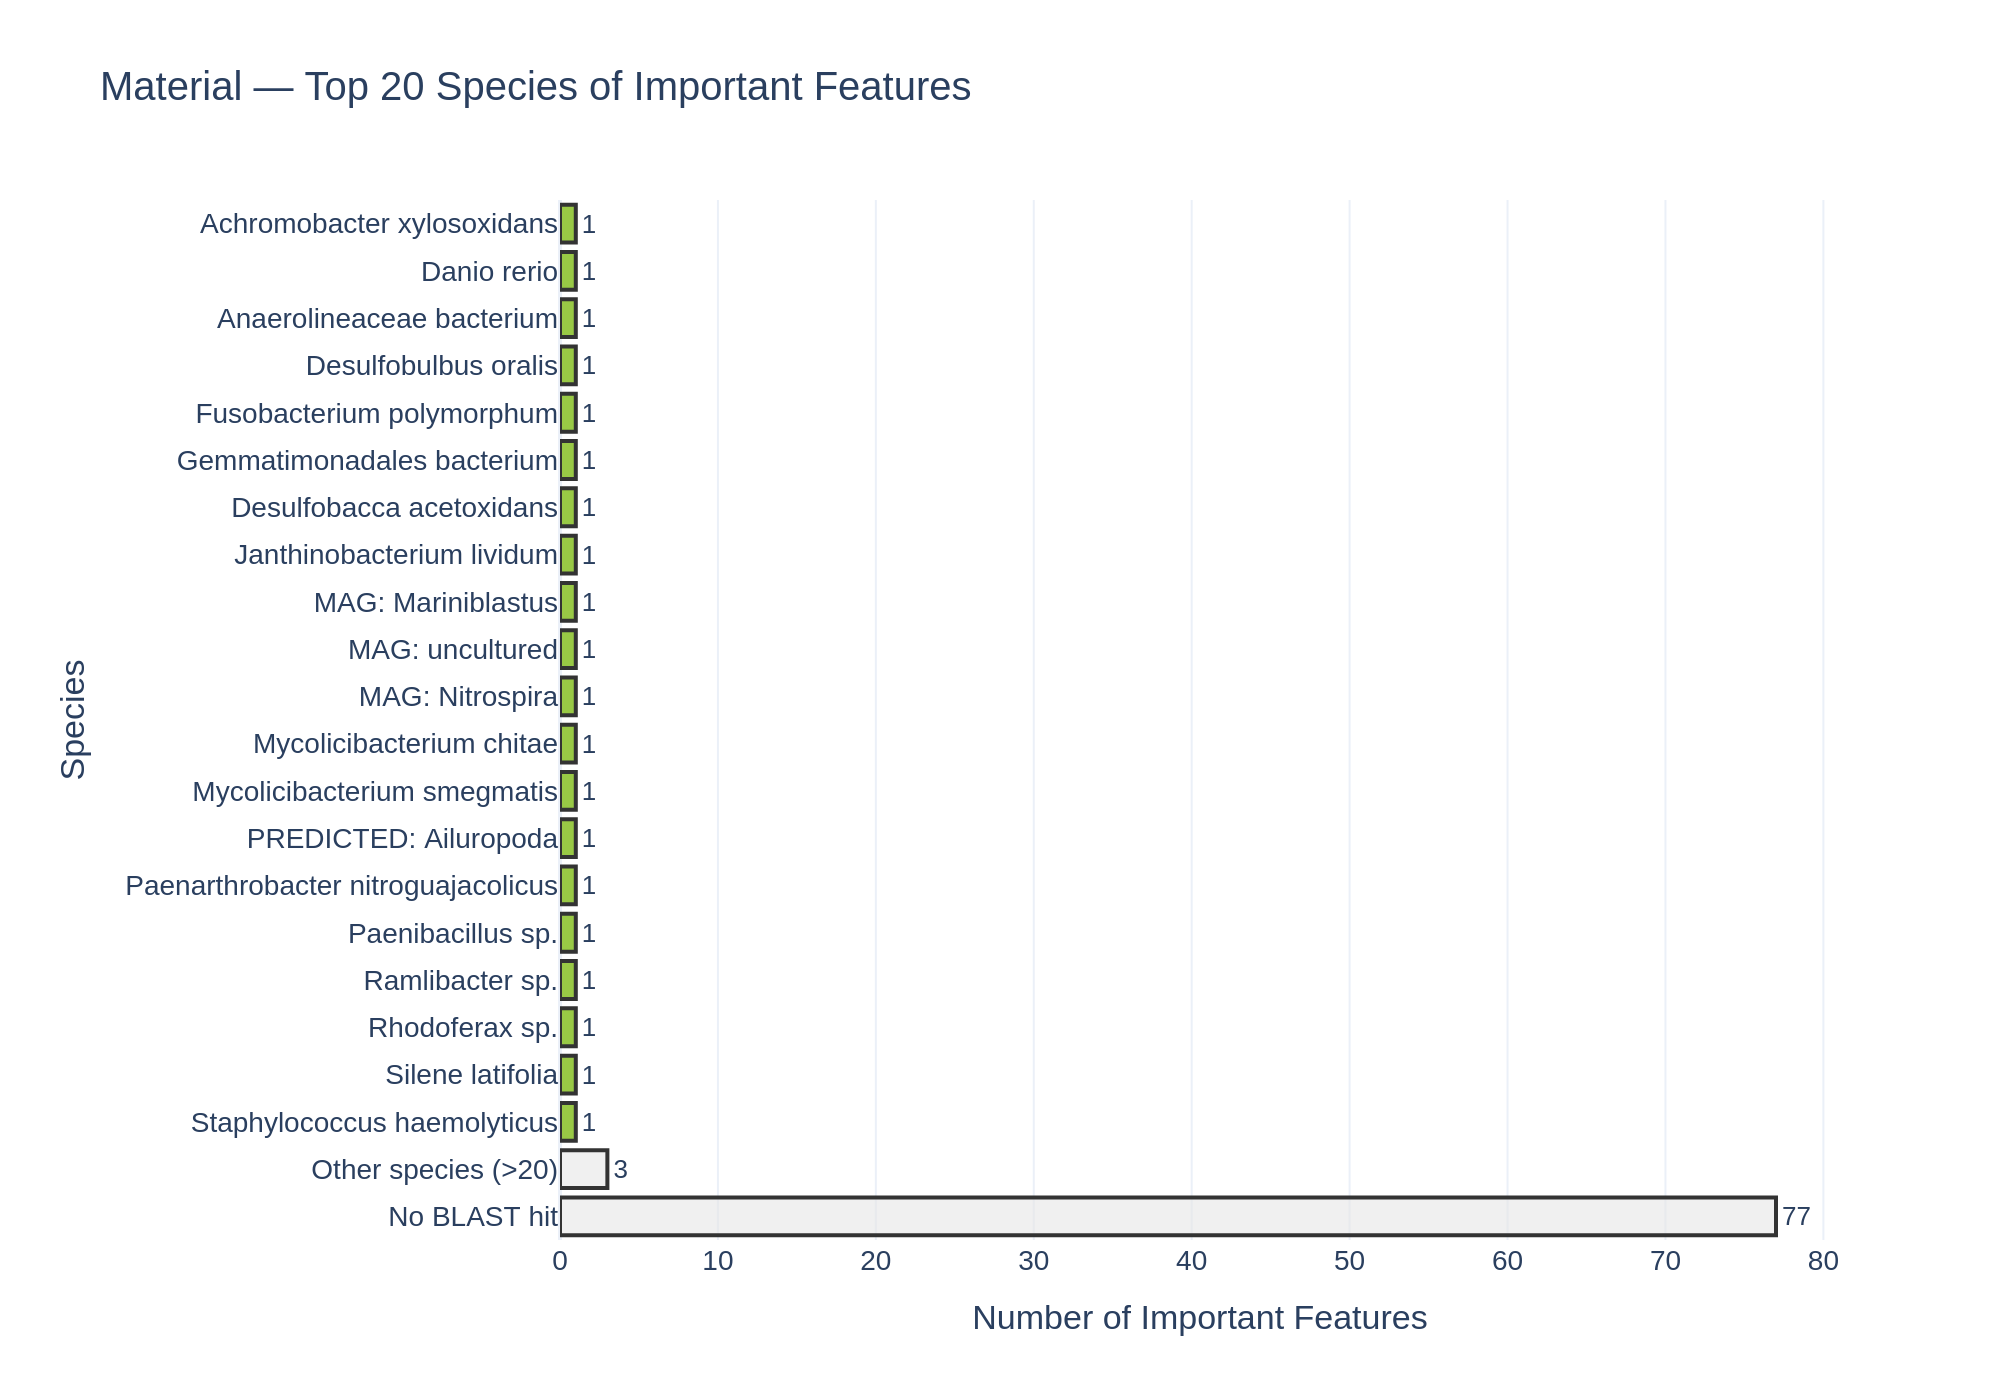
\includegraphics[width=0.49\textwidth]{main_03_feature_importance_material.png}%
    }
    \caption{\textbf{Top-15 most important unitig features per classification task, annotated by biological origin.}
    Lollipop plots showing the 15 highest-importance unitig features for each task:
    (a) Sample type, (b) Community type, (c) Sample host, and (d) Material.
    Feature importance is the mean gradient-based score across training epochs.
    Each feature is labelled with its species-level BLAST hit against the NCBI nt database
    (mean query coverage 98.3\%); the colour encodes the biological category of that annotation.
    Features marked \dag{} could not be matched by BLAST and were instead annotated via the
    Logan SRA genomic index (best hit by percent identity).
    Features labelled \textit{No annotation} are simple tandem repeats
    (e.g.\ $(\mathrm{AGT})_n$, $(\mathrm{CACT})_n$) that were masked in both databases.
    }
    \addcontentsline{toc}{subsection}{\protect\numberline{\thefigure}Feature importance by task}
    \label{fig:sup_feature_importance}
\end{figure}

\clearpage


%%%%%%%%%%%%%%%%%%%%%%%%%%%%%%%%%%%%%%%%%%%%%%%%%%%%%%%%%%%%%%%%%%%%%
%                      END OF SUPPLEMENTARY                         %
%%%%%%%%%%%%%%%%%%%%%%%%%%%%%%%%%%%%%%%%%%%%%%%%%%%%%%%%%%%%%%%%%%%%%

\end{document}
